\documentclass[11pt]{article}
\usepackage[margin=2cm]{geometry}
\usepackage{amsmath,amssymb}
\usepackage{graphicx}
\usepackage{booktabs}
\usepackage{array}
\usepackage{xcolor}
\usepackage[breakable]{tcolorbox}
\usepackage{enumitem}
\usepackage[hidelinks]{hyperref}
\allowdisplaybreaks
\setlength{\parindent}{0pt}
\setlength{\parskip}{4pt}
\definecolor{stepc}{HTML}{1F4E9E}
\definecolor{ansc}{HTML}{0B6E4F}
\newcommand{\solstep}[2]{\par\medskip{\color{stepc}\textbf{Step #1 --- #2}}\par\nopagebreak}
\newtcolorbox{probbox}[1]{colback=white,colframe=black!55,fonttitle=\bfseries,title={#1}}
\newtcolorbox{ansbox}{breakable,colback=ansc!6,colframe=ansc,fonttitle=\bfseries,title={Answer}}
\newtcolorbox{cardbox}[1]{breakable,colback=stepc!4,colframe=stepc,fonttitle=\bfseries,title={#1}}
\graphicspath{{../../../output/lecture2/2B_nodal_analysis/}}
\title{Set 2B: Op-Amp Circuits by Nodal Analysis}
\author{ECEN 325 --- Lecture 2 (Operational Amplifiers) practice set}
\date{}
\begin{document}
\maketitle

\textbf{What this set trains.} Op-amp circuits that are not one of the standard blocks. The recipe never changes:
apply the virtual short, write KCL at every node that is not an op-amp output, and eliminate the unknown node
voltages one at a time until only $V_o$ and $V_i$ are left. All op-amps are ideal. Problems 1--6 are easy, 7--12
medium, 13--18 hard. Try each problem before looking at its solution.


\begin{cardbox}{The Lecture-2 pipeline (use it for every problem in this lecture)}
\textbf{Tools --- this is all the theory you need (plus the Lecture-1 tools for impedances, dividers, Bode plots
and sinusoids):}
\begin{enumerate}[label=\textbf{T\arabic*},leftmargin=2.2em,itemsep=1pt]
\item \emph{Ideal op-amp with negative feedback:} no current into $+$ or $-$; $V_-=V_+$ (virtual short).
      Its output is an ideal voltage source (loads on it do not matter).
\item \emph{Block formulas:} inverting $\frac{V_o}{V_{in}}=-\frac{Z_f}{Z_{in}}$; non-inverting
      $\frac{V_o}{V_+}=1+\frac{Z_f}{Z_g}$ (with $V_+$ from the divider at the $+$ input); a follower has gain 1.
      Several blocks in cascade: multiply.
\item \emph{KCL with impedances:} at a node, $\sum_k \frac{V_{node}-V_k}{Z_k}=0$ (for a capacitor
      $\frac{1}{Z}=sC$). Write it at every node except op-amp outputs and source nodes.
\item \emph{Solving KCL equations:} pick the equation with the fewest unknowns, solve it for one node voltage,
      substitute into the rest; repeat until only $V_o$ and $V_i$ remain.
\item \emph{Finite gain:} $V_{out}=A(s)(V_+-V_-)$, $A(s)=\frac{A_0}{1+s/\omega_b}$, $\omega_t=A_0\omega_b$.
      With $V_+=\alpha_+V_{in}$, $V_-=\alpha_-V_{in}+\beta V_{out}$: $\frac{V_{out}}{V_{in}}=\frac{A(\alpha_+-\alpha_-)}{1+A\beta}$.
\item \emph{Slew rate:} for $V_{out}=\hat V\sin\omega t$, the fastest change is $\left|\frac{dV_{out}}{dt}\right|_{max}=\omega\hat V$;
      no distortion requires $\omega\hat V\le SR$.
\end{enumerate}
\textbf{Steps:}
\begin{enumerate}[leftmargin=2.2em,itemsep=1pt]
\item \emph{Sources.} DC and AC both present $\Rightarrow$ superposition.
\item \emph{DC circuit:} $V_i\to0$, $C\to$ open; pass the DC through each block with its gain at $s=0$.
\item \emph{Op-amp rules:} confirm negative feedback; apply T1 (or T5 for a non-ideal op-amp).
\item \emph{Transfer function:} standard blocks $\to$ T2; anything else $\to$ T3 + T4.
\item \emph{Standard form}, \ 6.~\emph{Bode}, \ 7.~\emph{Output} --- exactly as in Lecture 1.
\end{enumerate}
\emph{Variations:} a design problem runs these steps backwards (Bode plot $\to H(s)\to$ blocks $\to$ component values);
a slew-rate problem stops after Step 4 for every op-amp output and applies T6.
\end{cardbox}

\section*{Problems}
\subsection*{Easy problems}
\begin{probbox}{Problem 2B.1 \hfill Easy}
For the circuit below (ideal op-amps): (a) find $H(s)=\dfrac{V_o(s)}{V_i(s)}$ and sketch its magnitude Bode plot; (b) find the steady-state output $V_o(t)$ for $V_i(t) = 0.1\sin\left(2\pi\cdot 2000\,t\right)$.
\begin{center}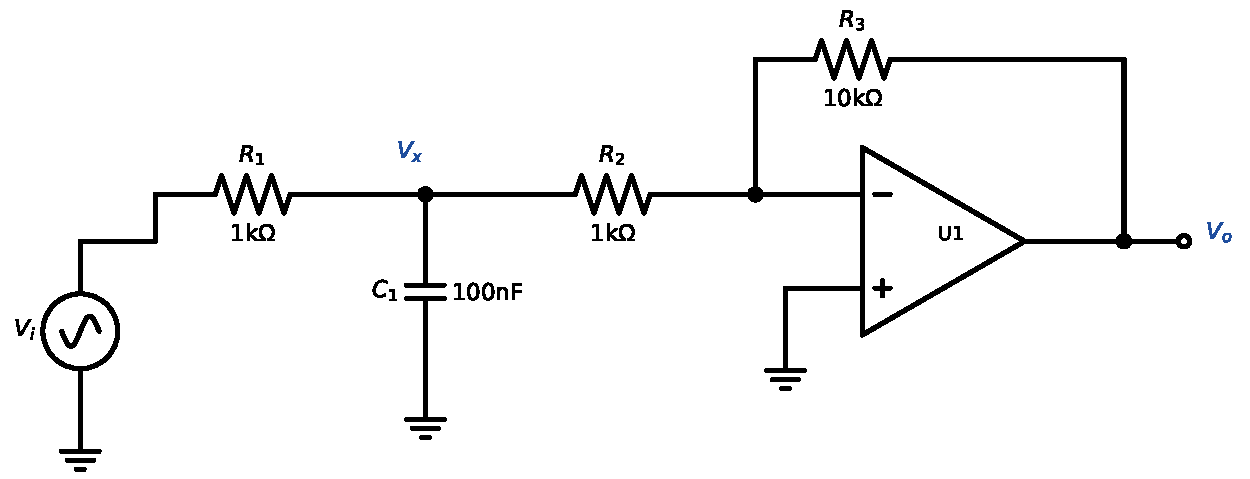
\includegraphics[width=\linewidth,height=5.6cm,keepaspectratio]{p01_circuit}\end{center}
\end{probbox}

\begin{probbox}{Problem 2B.2 \hfill Easy}
For the circuit below (ideal op-amps): (a) find $H(s)=\dfrac{V_o(s)}{V_i(s)}$ and sketch its magnitude Bode plot; (b) find the steady-state output $V_o(t)$ for $V_i(t) = 0.2\sin\left(2\pi\cdot 500\,t\right)$.
\begin{center}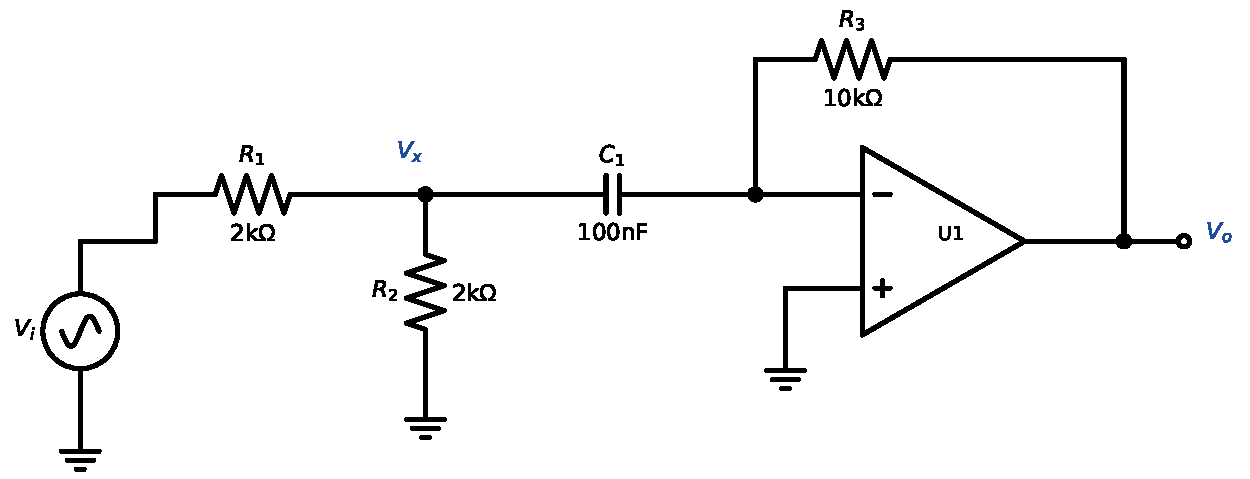
\includegraphics[width=\linewidth,height=5.6cm,keepaspectratio]{p02_circuit}\end{center}
\end{probbox}

\begin{probbox}{Problem 2B.3 \hfill Easy}
For the circuit below (ideal op-amps): (a) find $H(s)=\dfrac{V_o(s)}{V_i(s)}$ and sketch its magnitude Bode plot; (b) find the steady-state output $V_o(t)$ for $V_i(t) = 1\sin\left(2\pi\cdot 5000\,t\right)$.
\begin{center}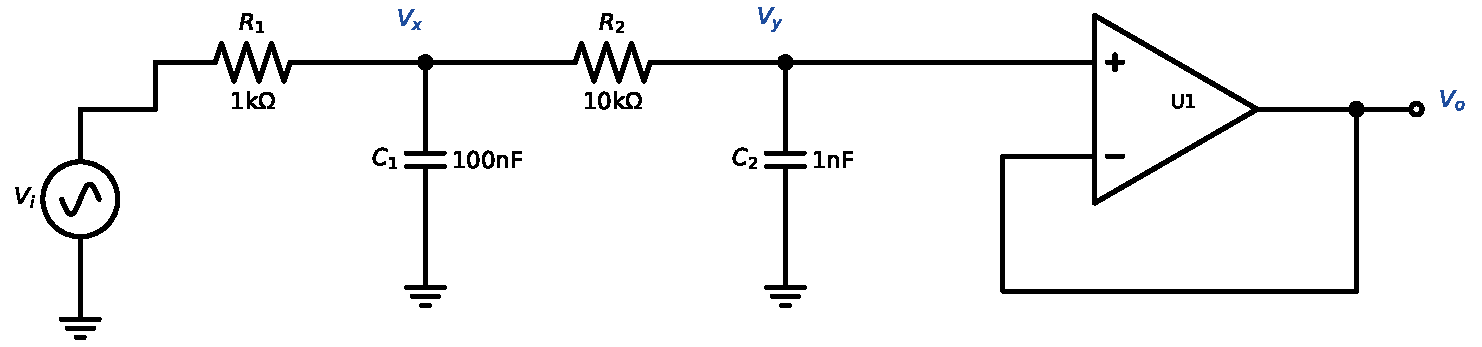
\includegraphics[width=\linewidth,height=5.6cm,keepaspectratio]{p03_circuit}\end{center}
\end{probbox}

\begin{probbox}{Problem 2B.4 \hfill Easy}
For the circuit below (ideal op-amps): (a) find $H(s)=\dfrac{V_o(s)}{V_i(s)}$ and sketch its magnitude Bode plot; (b) find the steady-state output $V_o(t)$ for $V_i(t) = 0.5\sin\left(2\pi\cdot 1000\,t\right)$.
\begin{center}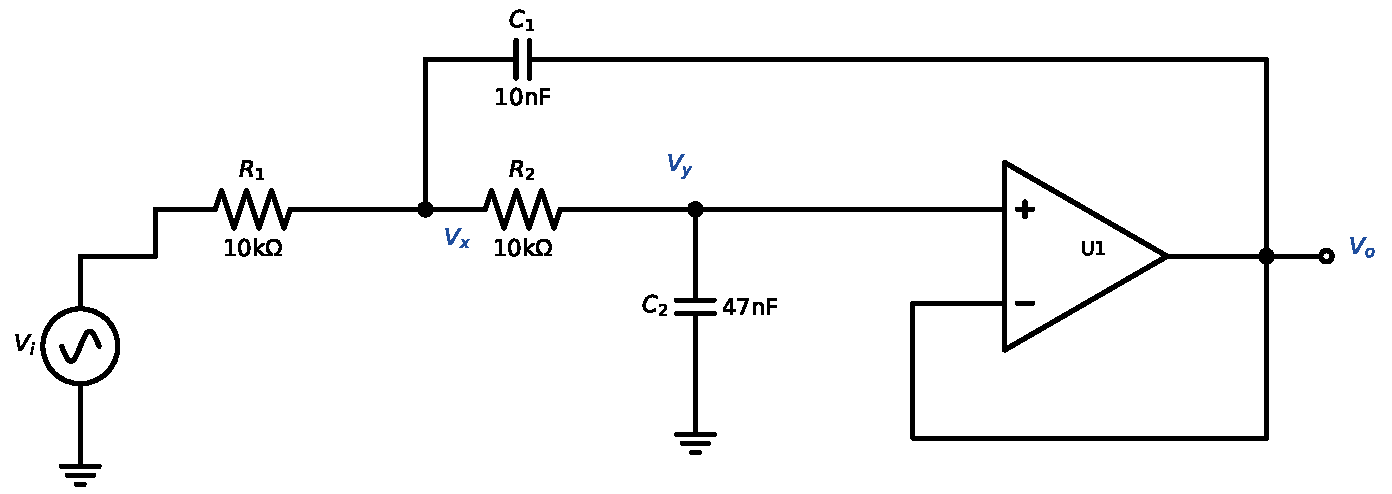
\includegraphics[width=\linewidth,height=5.6cm,keepaspectratio]{p04_circuit}\end{center}
\end{probbox}

\begin{probbox}{Problem 2B.5 \hfill Easy}
For the circuit below (ideal op-amps): (a) find $H(s)=\dfrac{V_o(s)}{V_i(s)}$ and sketch its magnitude Bode plot; (b) find the steady-state output $V_o(t)$ for $V_i(t) = 0.5\sin\left(2\pi\cdot 50000\,t\right)$.
\begin{center}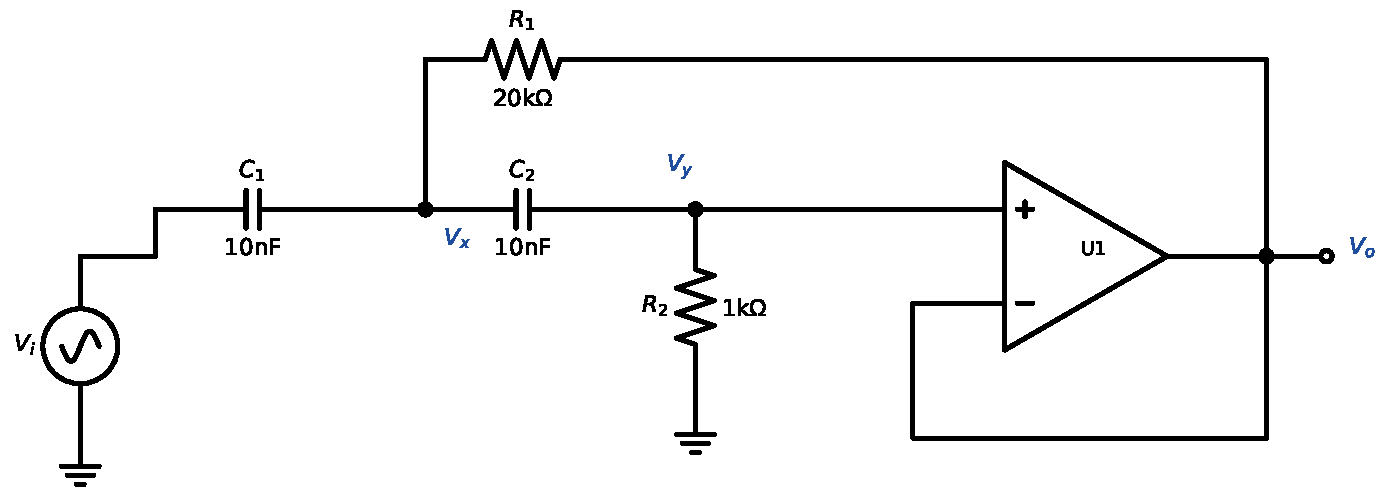
\includegraphics[width=\linewidth,height=5.6cm,keepaspectratio]{p05_circuit}\end{center}
\end{probbox}

\begin{probbox}{Problem 2B.6 \hfill Easy}
For the circuit below (ideal op-amps): (a) find $H(s)=\dfrac{V_o(s)}{V_i(s)}$ and sketch its magnitude Bode plot; (b) find the steady-state output $V_o(t)$ for $V_i(t) = 0.1\cos\left(2\pi\cdot 500\,t\right)$.
\begin{center}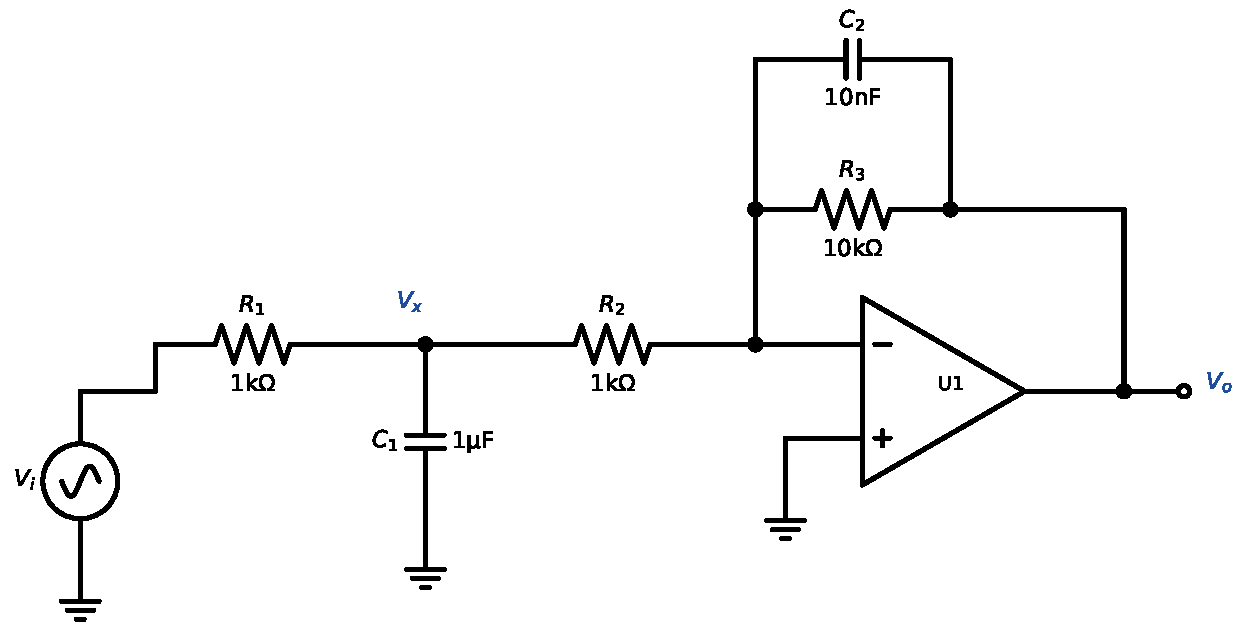
\includegraphics[width=\linewidth,height=5.6cm,keepaspectratio]{p06_circuit}\end{center}
\end{probbox}

\subsection*{Medium problems}
\begin{probbox}{Problem 2B.7 \hfill Medium}
For the circuit below (ideal op-amps): (a) find $H(s)=\dfrac{V_o(s)}{V_i(s)}$ and sketch its magnitude Bode plot; (b) find the steady-state output $V_o(t)$ for $V_i(t) = 0.2\sin\left(2\pi\cdot 1000\,t\right)$.
\begin{center}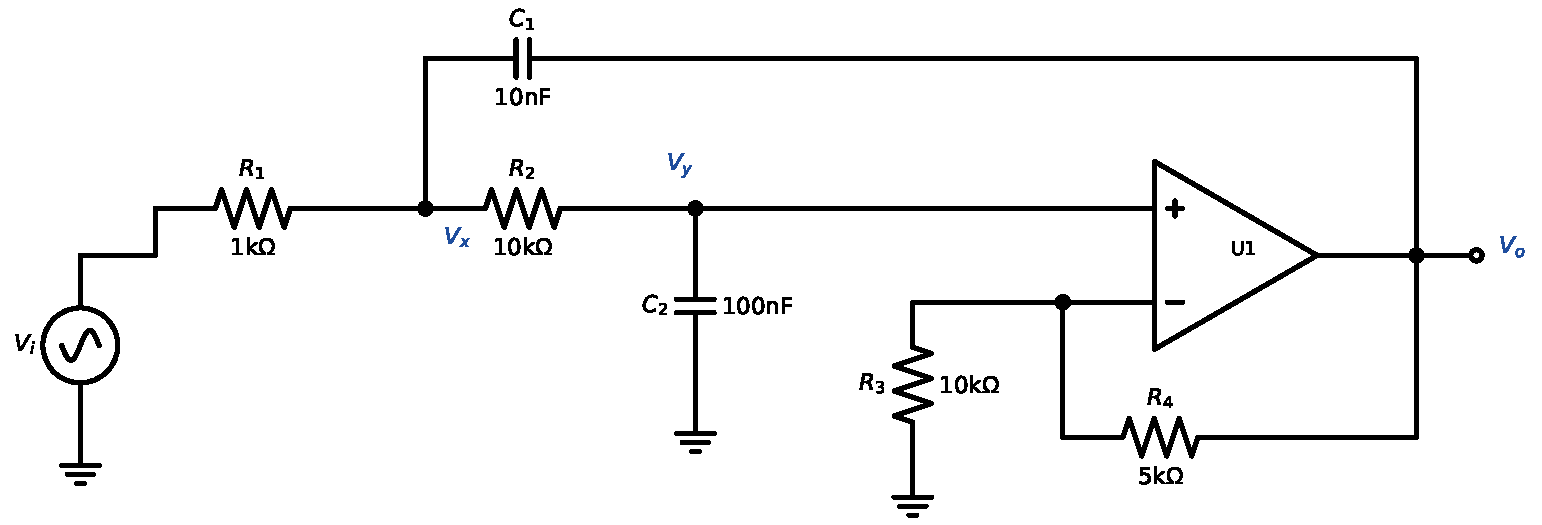
\includegraphics[width=\linewidth,height=5.6cm,keepaspectratio]{p07_circuit}\end{center}
\end{probbox}

\begin{probbox}{Problem 2B.8 \hfill Medium}
For the circuit below (ideal op-amps): (a) find $H(s)=\dfrac{V_o(s)}{V_i(s)}$ and sketch its magnitude Bode plot; (b) find the steady-state output $V_o(t)$ for $V_i(t) = 0.2\sin\left(2\pi\cdot 30000\,t\right)$.
\begin{center}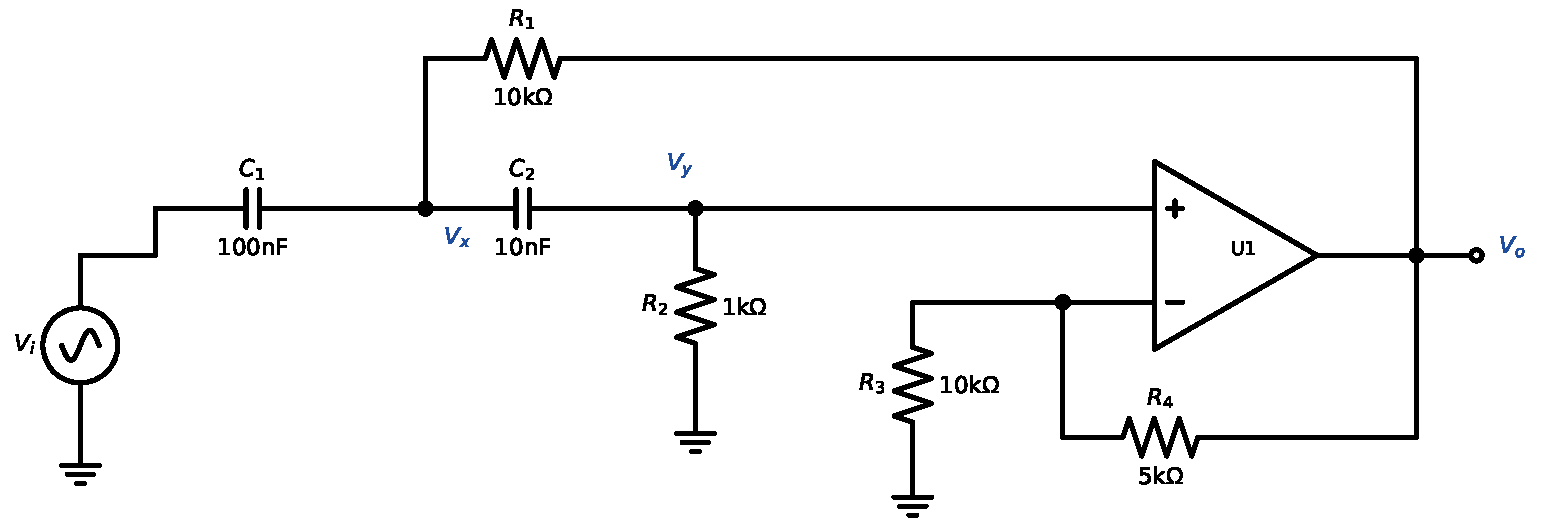
\includegraphics[width=\linewidth,height=5.6cm,keepaspectratio]{p08_circuit}\end{center}
\end{probbox}

\begin{probbox}{Problem 2B.9 \hfill Medium}
For the circuit below (ideal op-amps): (a) find $H(s)=\dfrac{V_o(s)}{V_i(s)}$ and sketch its magnitude Bode plot; (b) find the steady-state output $V_o(t)$ for $V_i(t) = 1\sin\left(2\pi\cdot 300\,t\right)$.
\begin{center}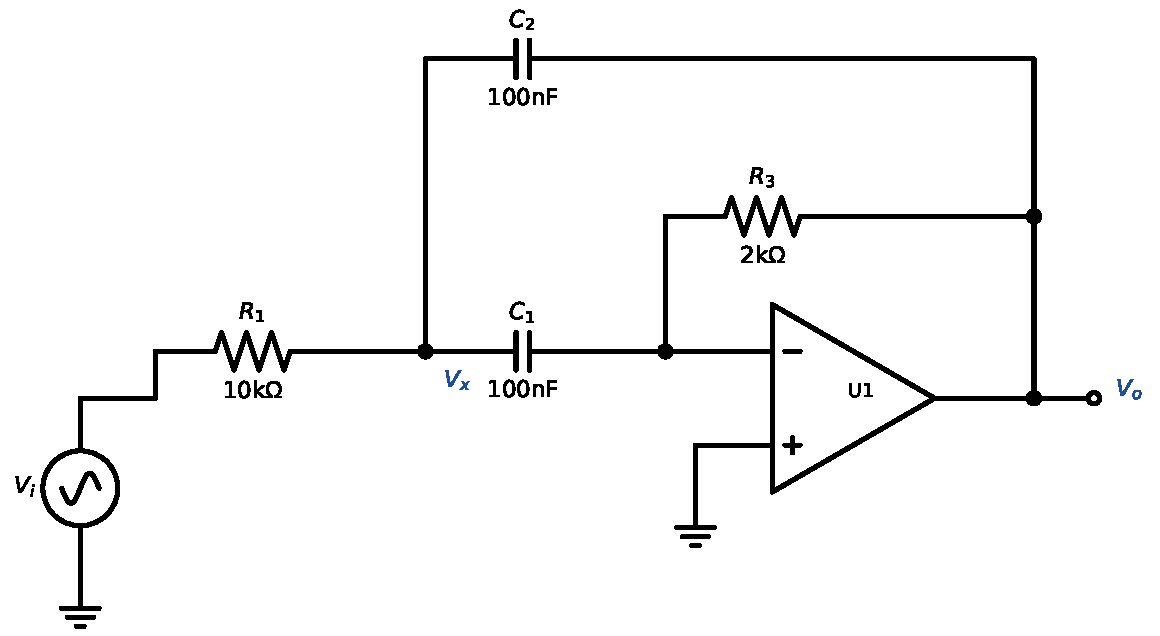
\includegraphics[width=\linewidth,height=5.6cm,keepaspectratio]{p09_circuit}\end{center}
\end{probbox}

\begin{probbox}{Problem 2B.10 \hfill Medium}
For the circuit below (ideal op-amps): (a) find $H(s)=\dfrac{V_o(s)}{V_i(s)}$ and sketch its magnitude Bode plot; (b) find the steady-state output $V_o(t)$ for $V_i(t) = 0.5\sin\left(2\pi\cdot 200\,t\right)$.
\begin{center}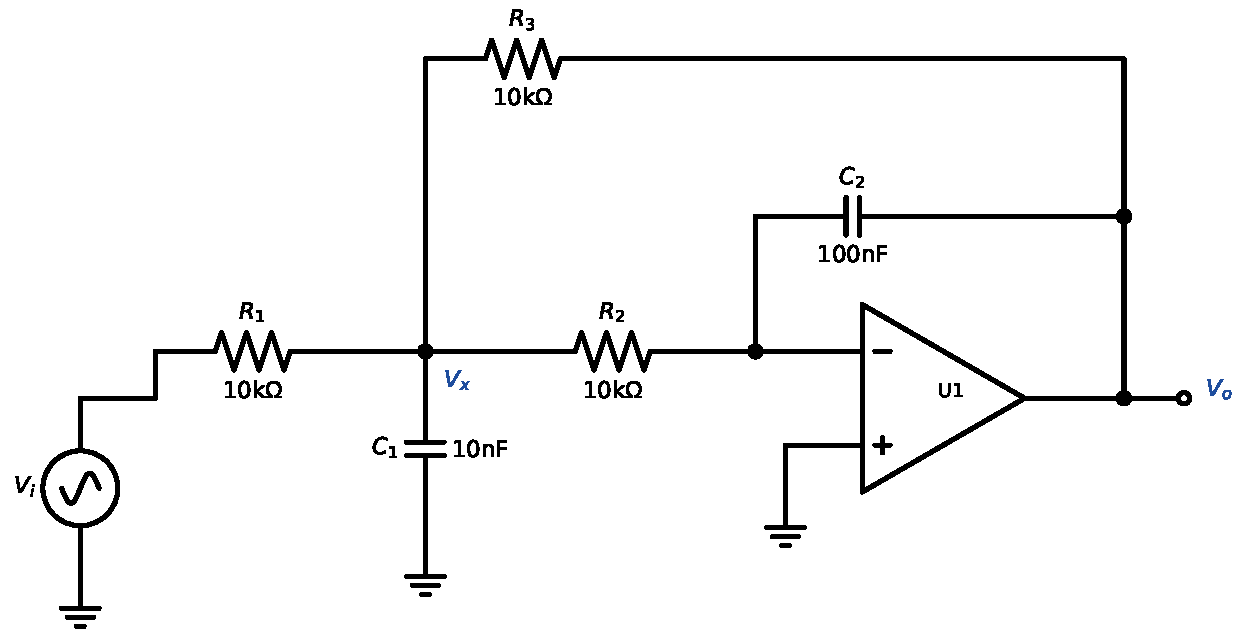
\includegraphics[width=\linewidth,height=5.6cm,keepaspectratio]{p10_circuit}\end{center}
\end{probbox}

\begin{probbox}{Problem 2B.11 \hfill Medium}
For the circuit below (ideal op-amps): (a) find $H(s)=\dfrac{V_o(s)}{V_i(s)}$ and sketch its magnitude Bode plot; (b) find the steady-state output $V_o(t)$ for $V_i(t) = 0.5\sin\left(2\pi\cdot 500\,t+\frac{\pi}{4}\right)$.
\begin{center}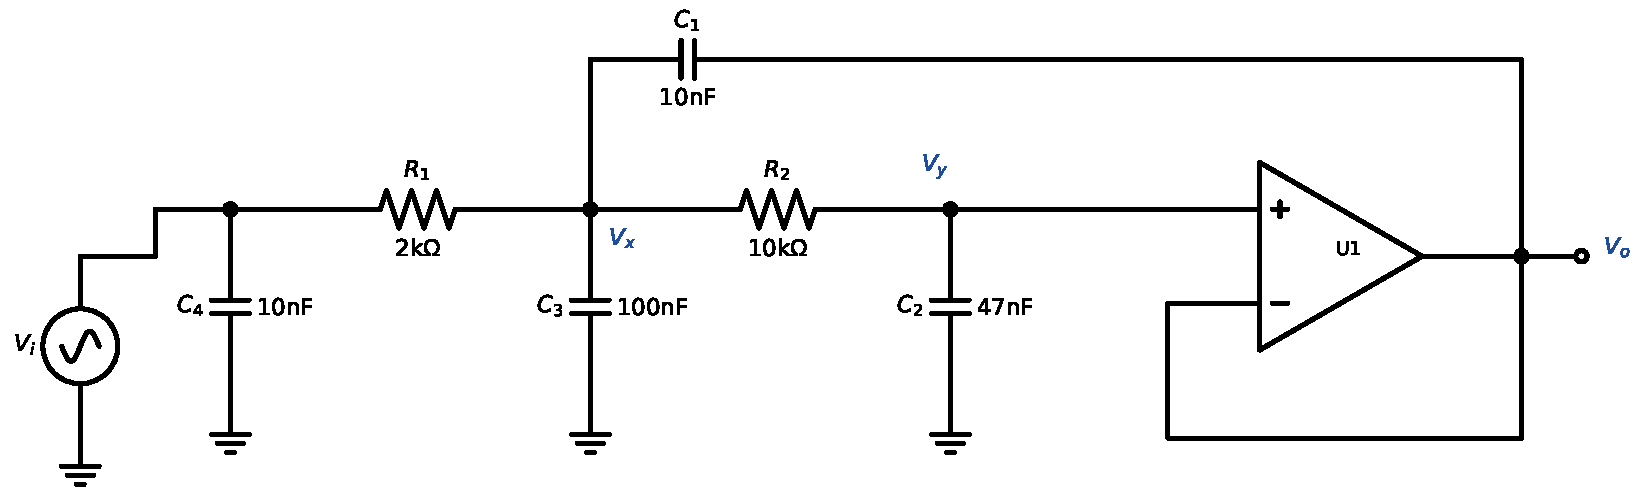
\includegraphics[width=\linewidth,height=5.6cm,keepaspectratio]{p11_circuit}\end{center}
\end{probbox}

\begin{probbox}{Problem 2B.12 \hfill Medium}
For the circuit below (ideal op-amps): (a) find $H(s)=\dfrac{V_o(s)}{V_i(s)}$ and sketch its magnitude Bode plot; (b) find the steady-state output $V_o(t)$ for $V_i(t) = 0.1\sin\left(2\pi\cdot 1000\,t\right)$.
\begin{center}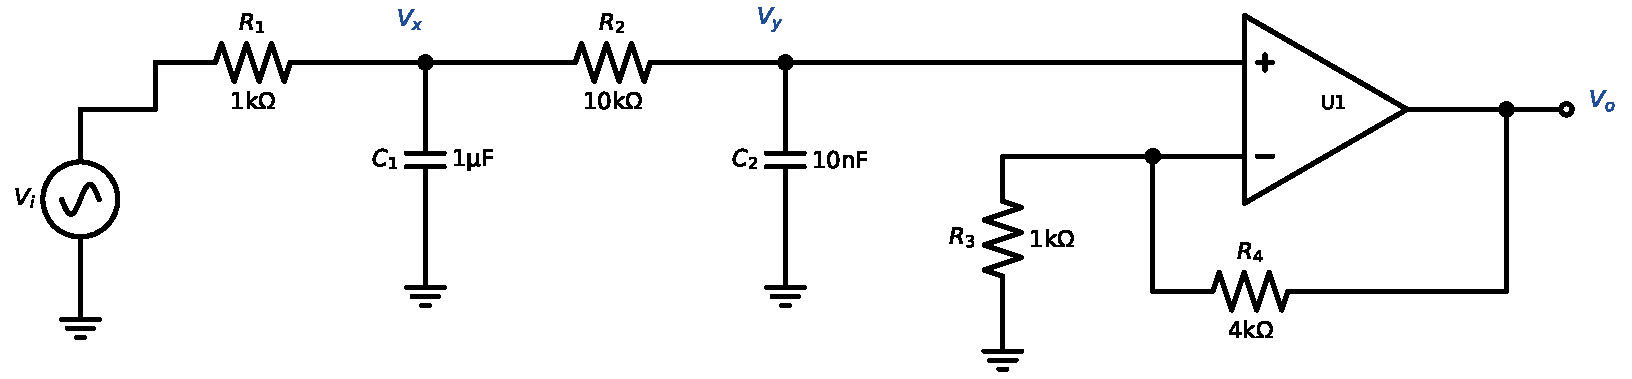
\includegraphics[width=\linewidth,height=5.6cm,keepaspectratio]{p12_circuit}\end{center}
\end{probbox}

\subsection*{Hard problems}
\begin{probbox}{Problem 2B.13 \hfill Hard}
For the circuit below (ideal op-amps): (a) find $H(s)=\dfrac{V_o(s)}{V_i(s)}$ and sketch its magnitude Bode plot; (b) find the steady-state output $V_o(t)$ for $V_i(t) = 0.1\sin\left(2\pi\cdot 2000\,t\right)$.
\begin{center}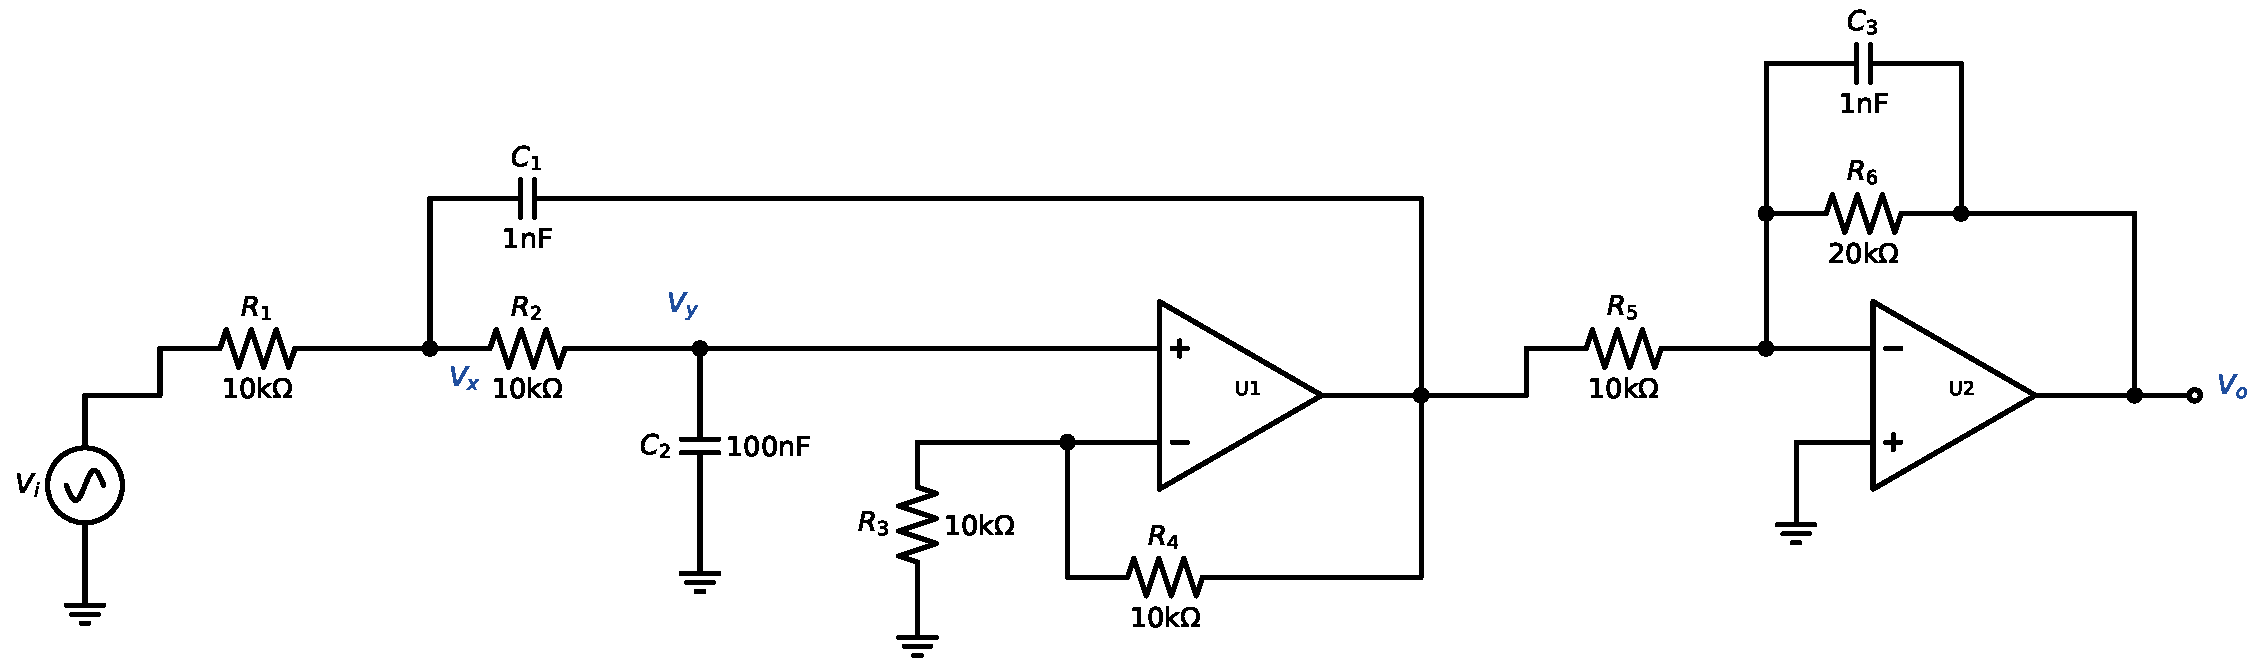
\includegraphics[width=\linewidth,height=5.6cm,keepaspectratio]{p13_circuit}\end{center}
\end{probbox}

\begin{probbox}{Problem 2B.14 \hfill Hard}
For the circuit below (ideal op-amps): (a) find $H(s)=\dfrac{V_o(s)}{V_i(s)}$ and sketch its magnitude Bode plot; (b) find the steady-state output $V_o(t)$ for $V_i(t) = 0.05\sin\left(2\pi\cdot 2000\,t\right)$.
\begin{center}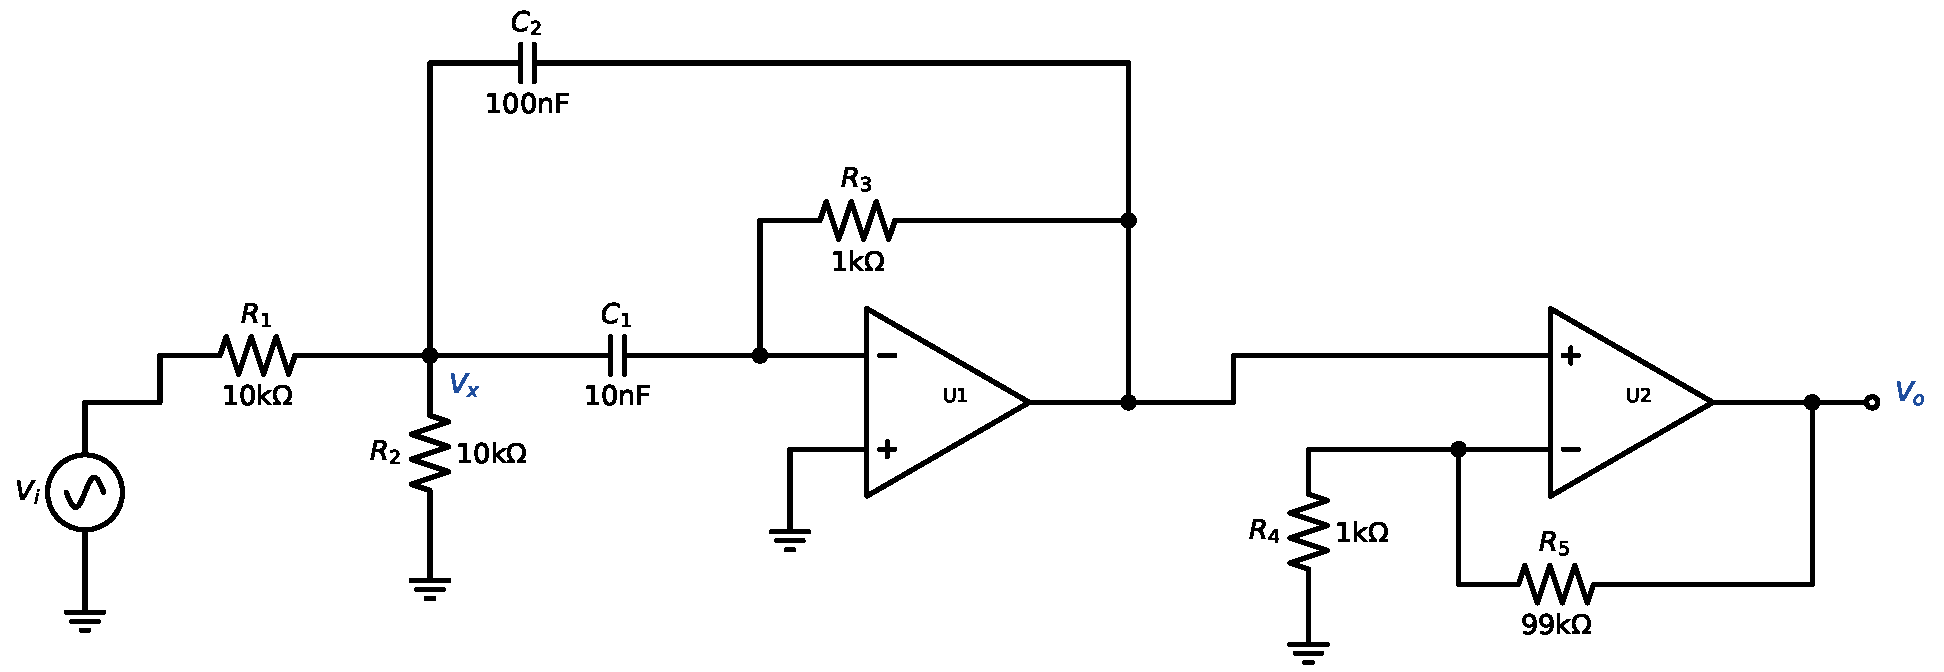
\includegraphics[width=\linewidth,height=5.6cm,keepaspectratio]{p14_circuit}\end{center}
\end{probbox}

\begin{probbox}{Problem 2B.15 \hfill Hard}
For the circuit below (ideal op-amps): (a) find $H(s)=\dfrac{V_o(s)}{V_i(s)}$ and sketch its magnitude Bode plot; (b) find the steady-state output $V_o(t)$ for $V_i(t) = 0.05\sin\left(2\pi\cdot 1000\,t\right)$.
\begin{center}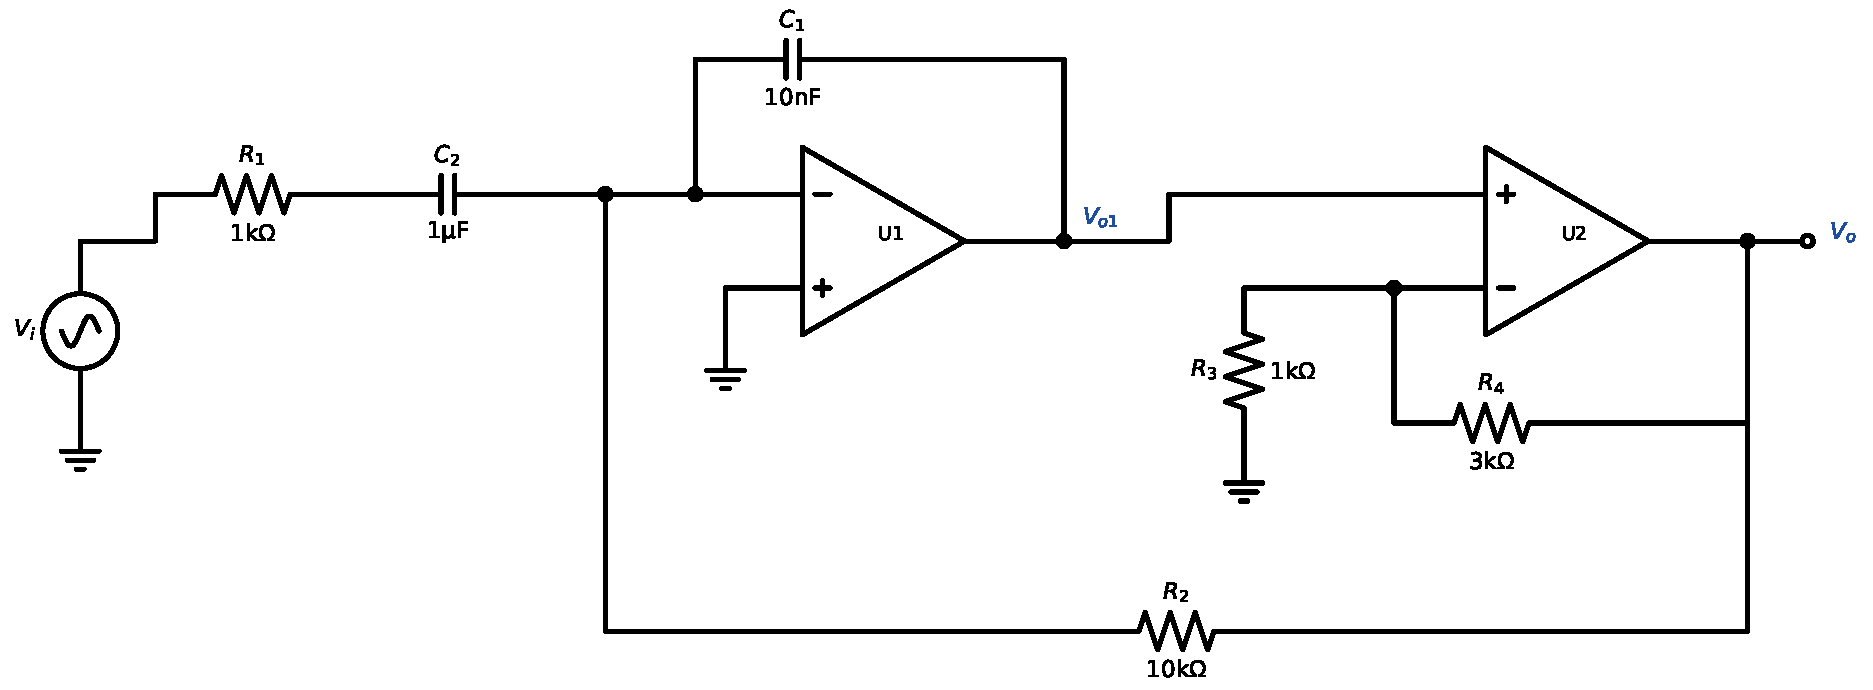
\includegraphics[width=\linewidth,height=5.6cm,keepaspectratio]{p15_circuit}\end{center}
\end{probbox}

\begin{probbox}{Problem 2B.16 \hfill Hard}
For the circuit below (ideal op-amps): (a) find $H(s)=\dfrac{V_o(s)}{V_i(s)}$ and sketch its magnitude Bode plot; (b) find the steady-state output $V_o(t)$ for $V_i(t) = 0.2\cos\left(2\pi\cdot 5000\,t-\frac{\pi}{4}\right)$.
\begin{center}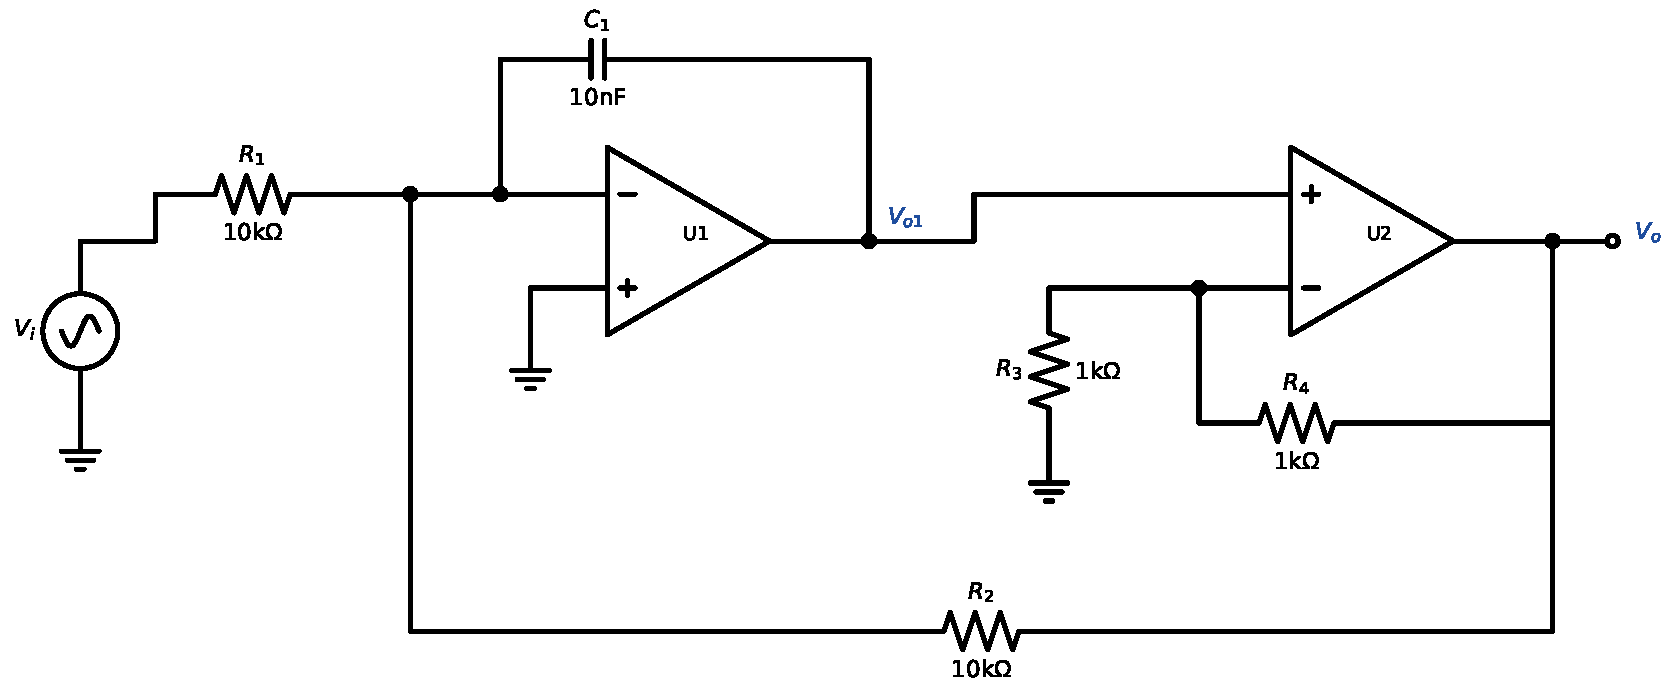
\includegraphics[width=\linewidth,height=5.6cm,keepaspectratio]{p16_circuit}\end{center}
\end{probbox}

\begin{probbox}{Problem 2B.17 \hfill Hard}
For the circuit below (ideal op-amps): (a) find $H(s)=\dfrac{V_o(s)}{V_i(s)}$ and sketch its magnitude Bode plot; (b) find the steady-state output $V_o(t)$ for $V_i(t) = 0.1\sin\left(2\pi\cdot 20000\,t\right)$.
\begin{center}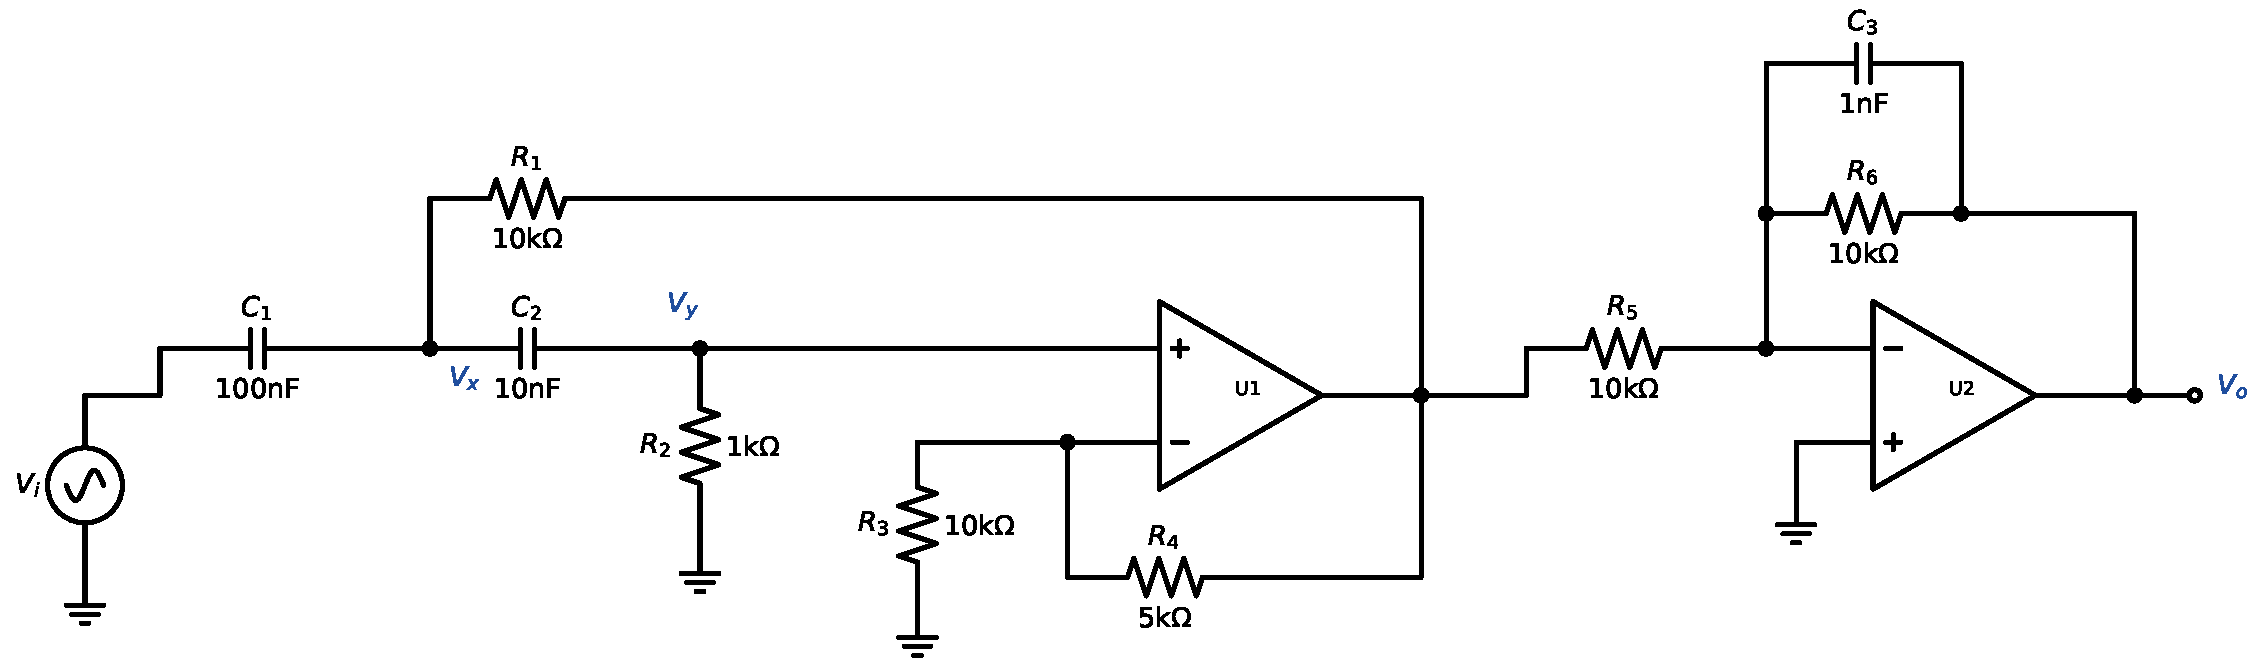
\includegraphics[width=\linewidth,height=5.6cm,keepaspectratio]{p17_circuit}\end{center}
\end{probbox}

\begin{probbox}{Problem 2B.18 \hfill Hard}
For the circuit below (ideal op-amps): (a) find $H(s)=\dfrac{V_o(s)}{V_i(s)}$ and sketch its magnitude Bode plot; (b) find the steady-state output $V_o(t)$ for $V_i(t) = 0.05\sin\left(2\pi\cdot 1000\,t+\frac{\pi}{3}\right)$.
\begin{center}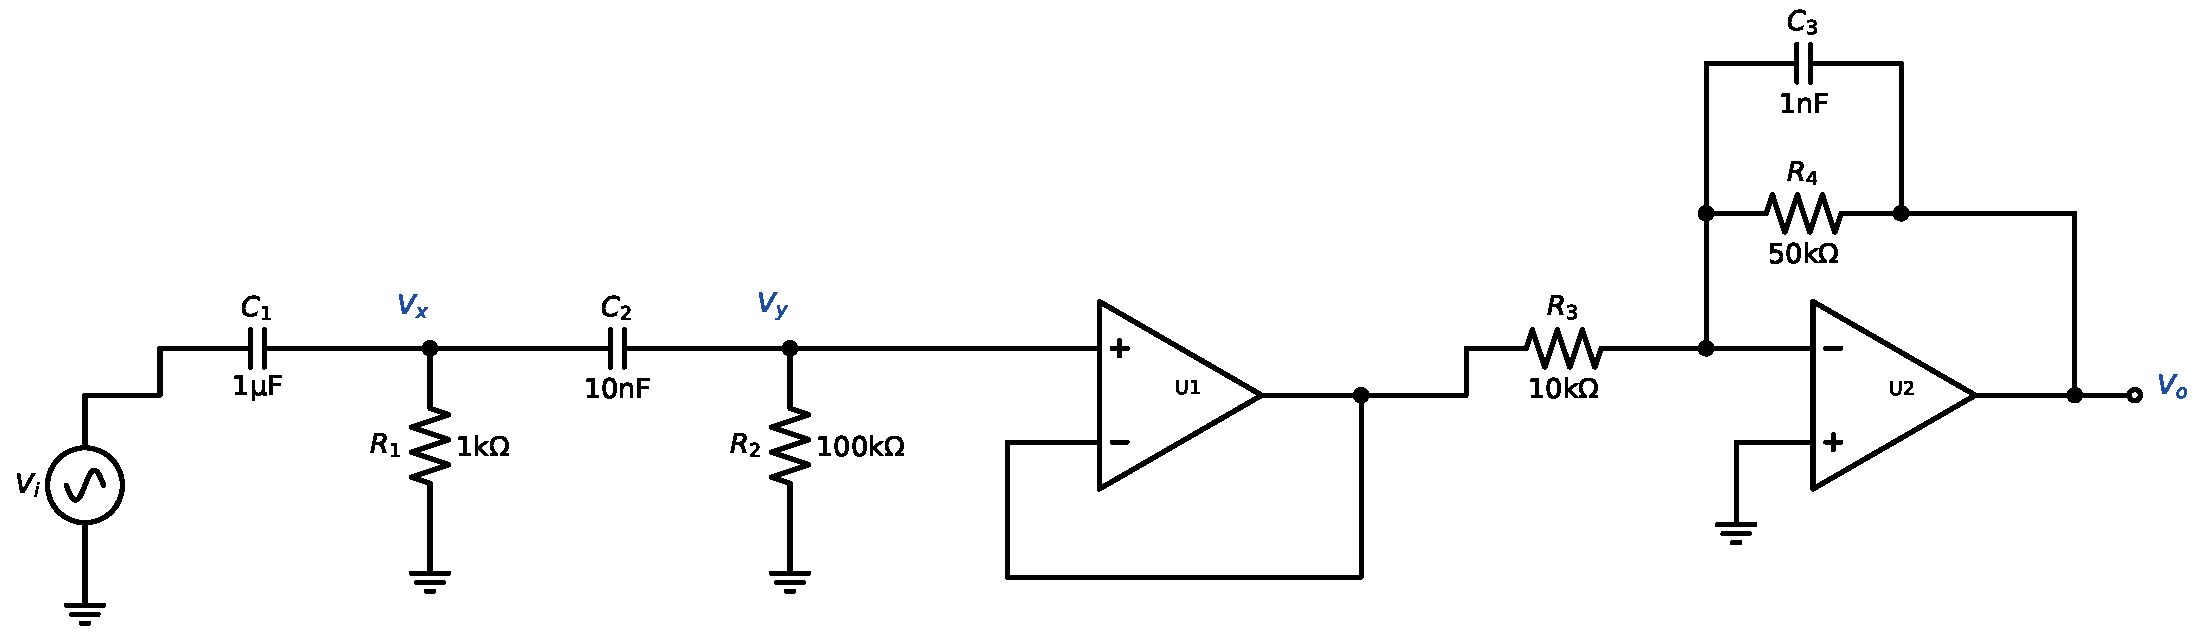
\includegraphics[width=\linewidth,height=5.6cm,keepaspectratio]{p18_circuit}\end{center}
\end{probbox}

\newpage
\section*{Solutions}
Every solution follows the steps of the Lecture-2 pipeline card.
\newpage
\subsection*{Solution 2B.1 \hfill Easy}
\begin{center}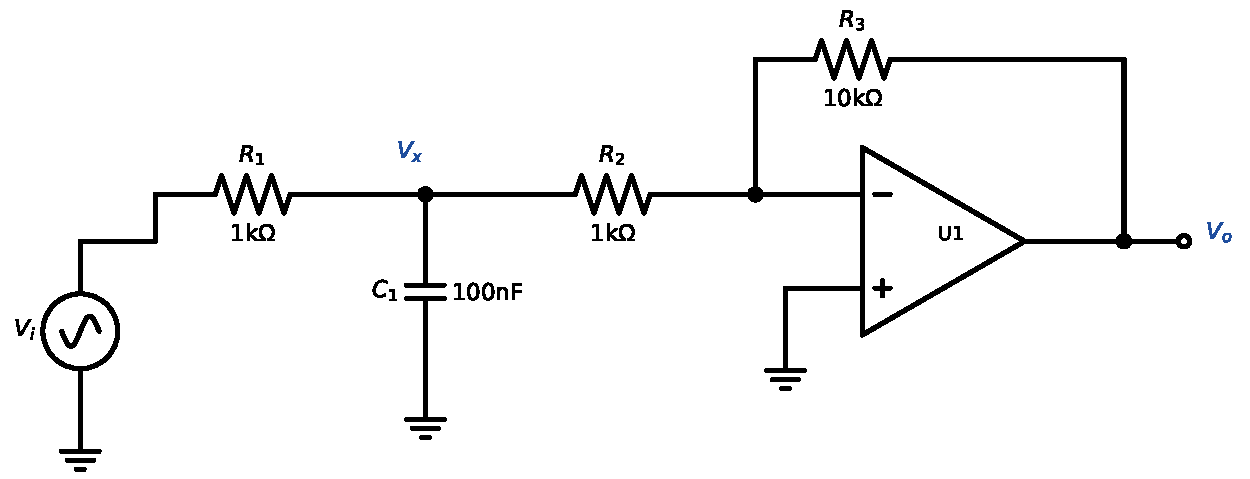
\includegraphics[width=\linewidth,height=5cm,keepaspectratio]{p01_circuit}\end{center}
\solstep{1}{Identify the sources}Independent sources: the AC input $V_i(t)$. No DC source: $V_{o,dc}=0$ and Step 2 is skipped.
\solstep{2}{DC circuit}No DC sources: $V_{o,dc}=0$.
\solstep{3}{Op-amp rules}Each op-amp has negative feedback (its output is connected back to its $-$ input), so with an ideal op-amp (tool T1): (a) no current flows into the $+$ or $-$ input; (b) $V_-=V_+$ (virtual short). The circuit is not a standard block, so it is solved by nodal analysis (tools T3, T4).
\solstep{4}{Transfer function by nodal analysis}\textbf{Block 1 (U1).} Inverting amplifier whose input network has a shunt branch. This is not a standard block, so use nodal analysis. Virtual short (tool T1): U1: $V_- = V_+$, so $V_{-}$ is the same voltage as $0$ (virtual ground).
KCL (tool T3) at every node that is not an op-amp output or a source; no current flows into the op-amp inputs, so the op-amps do not appear in these sums:
\begin{align*}
&\text{(1) at }V_{-}\,(=0): && \frac{0 - V_{x}}{R_{2}} + \frac{0 - V_{o}}{R_{3}} = 0 \\
&\text{(2) at }V_{x}: && \frac{V_{x} - V_{i}}{R_{1}} + sC_{1}V_{x} + \frac{V_{x}}{R_{2}} = 0
\end{align*}

Solve them one at a time (tool T4): take the equation with the fewest unknowns, solve it for one node voltage and substitute that into the remaining equations. With the component values:
\begin{align*}
\text{from (2):}\quad V_{x} &= \left(\dfrac{10000}{s + 20000}\right)V_i
\end{align*}

Substituting everything into (1) leaves only $V_{o}$ and $V_i$.\[
\frac{V_{o}}{V_i} = \dfrac{-10^{5}}{s + 20000}
\]

So:\[
H(s) = \dfrac{-10^{5}}{s + 20000}
\]

\solstep{5}{Standard (Bode-ready) form}Find the roots. Every root $s=-p$ of the denominator is a \emph{pole}, every root $s=-z$ of the numerator is a \emph{zero}; $|p|$ and $|z|$ are the corner frequencies (rad/s).
\begin{itemize}[leftmargin=*,itemsep=2pt]
\item Denominator: $s + 20000$; $s + 20000 = 0 \Rightarrow s = -20000$.
\end{itemize}

Factored form (leading coefficient in front):
\[
H(s) = -10^{5}\,\dfrac{1}{(s+20000)}
\]

Bode-ready form: rewrite every $(s+p) = p\left(1+\frac{s}{p}\right)$ and $(s+z) = z\left(1+\frac{s}{z}\right)$, and collect all constants into $K$. Then every factor except $K$ is $\approx 1$ inside the pass-band:
\[
H(s) = -5\,\dfrac{1}{1+\dfrac{s}{2\pi\cdot 3.18\mathrm{k}}},\qquad K = -5
\]

\begin{center}\renewcommand{\arraystretch}{1.35}
\begin{tabular}{cccc}
\toprule
type & $\omega_c$ (rad/s) & $f_c=\omega_c/2\pi$ & slope change \\
\midrule
pole & $20000$ & 3.18 kHz & $-20$ dB/dec \\
\bottomrule
\end{tabular}\end{center}

\solstep{6}{Magnitude Bode plot}Below every corner, all factors are $\approx$ constant: $|H| \approx 5$ $= 14$\,dB (flat, 0 dB/dec). Then, moving right, each pole bends the line down by 20\,dB/dec and each zero bends it up by 20\,dB/dec (tool T6):
\begin{center}\renewcommand{\arraystretch}{1.35}
\begin{tabular}{lcl}
\toprule
frequency range & slope & asymptote level \\
\midrule
$f<$ 3.18 kHz & $0$ dB/dec (flat) & 14 dB at end \\
$f>$ 3.18 kHz & $-20$ dB/dec & 14 dB at start \\
\bottomrule
\end{tabular}\end{center}

The flat (pass-band) level is $20\log_{10}|K| = 20\log_{10}5 = 14$\,dB.
\begin{center}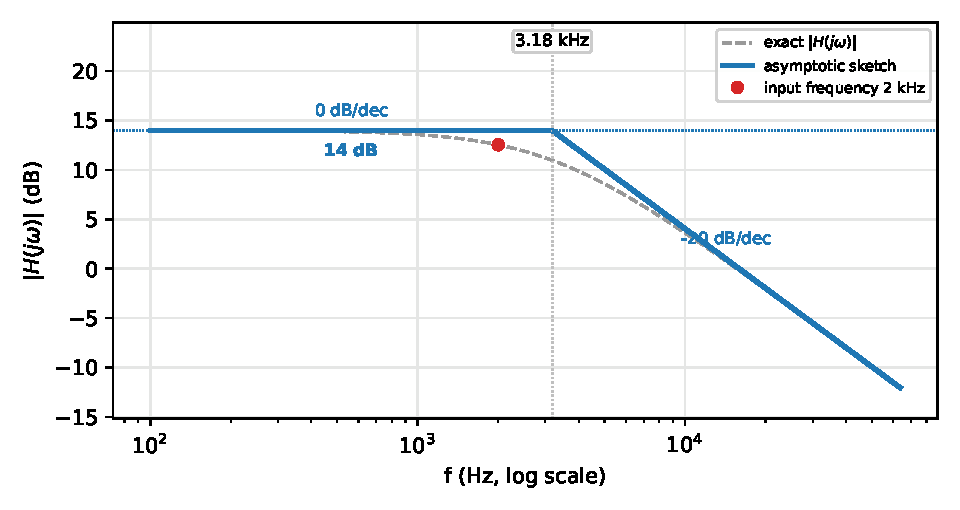
\includegraphics[width=0.78\linewidth,height=6.5cm,keepaspectratio]{p01_bode}\end{center}

{\small Blue: the straight-line sketch you are expected to draw. Dashed grey: the exact curve (about 3\,dB below the corner of an isolated pole). Red dot: the input frequency of Step 7.}
\solstep{7}{Steady-state output}The input is $V_i(t) = 0.1\sin\left(2\pi\cdot 2000\,t\right)$, so $\omega_{in} = 2\pi\cdot 2000 = 12600$\,rad/s. Put $s=j\omega_{in}$ in each factor (tool T5): magnitudes multiply, angles add.
{\small Rules: $\left|\frac{s}{s+p}\right| = \frac{\omega}{\sqrt{\omega^2+p^2}}$, $\angle = \frac{\pi}{2}-\tan^{-1}\frac{\omega}{p}$;\quad $\left|\frac{1}{1+s/p}\right| = \frac{1}{\sqrt{1+(\omega/p)^2}}$, $\angle = -\tan^{-1}\frac{\omega}{p}$;\quad $\left|1+\frac{s}{z}\right| = \sqrt{1+(\omega/z)^2}$, $\angle = \tan^{-1}\frac{\omega}{z}$;\quad a negative $K$ adds $-\pi$.}
\begin{center}\renewcommand{\arraystretch}{1.35}
\begin{tabular}{ccc}
\toprule
factor & magnitude & angle (rad) \\
\midrule
$-5$ & $5$ & $-3.14$ \\
$\rule[-1.7em]{0pt}{4em}\dfrac{1}{1+\dfrac{s}{2\pi\cdot 3.18\mathrm{k}}}$ & $0.8467$ & $-0.561$ \\
\textbf{total} & $\mathbf{4.234}$ (product) & $\mathbf{-3.7}$ (sum) \\
\bottomrule
\end{tabular}\end{center}

\begin{align*}
|H(j\omega_{in})| &= 4.23, \qquad \angle H(j\omega_{in}) = -3.7\ \mathrm{rad} \\
v_{o,ac}(t) &= 4.23\times 0.1\,\sin\left(2\pi\cdot 2000\,t - 3.7\right) = 0.423\,\sin\left(2\pi\cdot 2000\,t - 3.7\right)
\end{align*}

\[
\boxed{V_o(t) = 0.423\,\sin\left(2\pi\cdot 2000\,t - 3.7\right)\ \mathrm{V}}
\]

\begin{ansbox}
$H(s) = -5\,\dfrac{1}{1+\dfrac{s}{2\pi\cdot 3.18\mathrm{k}}}$\quad (corners: 3.18 kHz)\\[4pt]
$V_o(t) = 0.423\,\sin\left(2\pi\cdot 2000\,t - 3.7\right)\ \mathrm{V}$
\end{ansbox}

\newpage
\subsection*{Solution 2B.2 \hfill Easy}
\begin{center}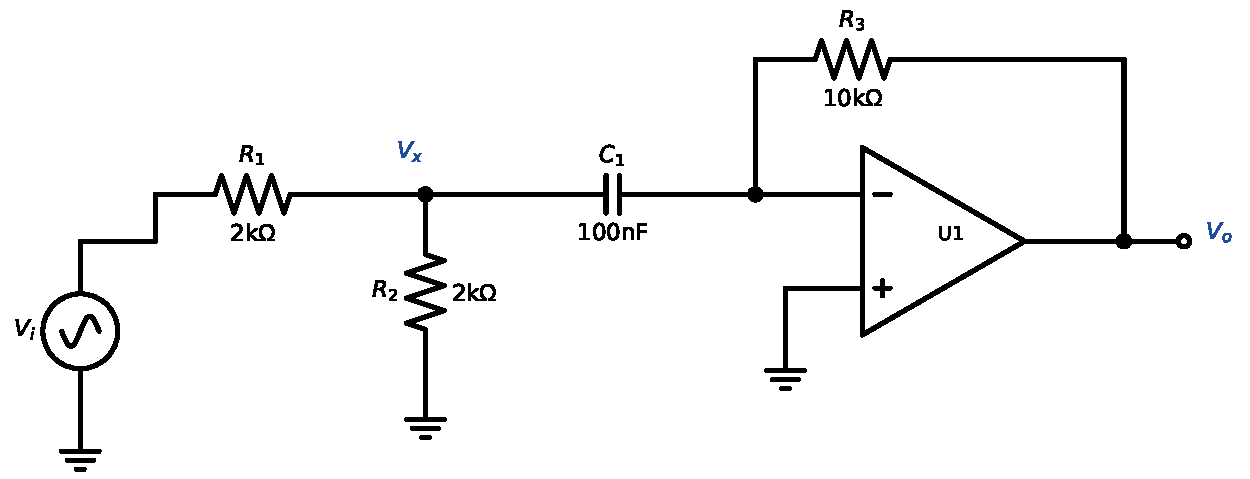
\includegraphics[width=\linewidth,height=5cm,keepaspectratio]{p02_circuit}\end{center}
\solstep{1}{Identify the sources}Independent sources: the AC input $V_i(t)$. No DC source: $V_{o,dc}=0$ and Step 2 is skipped.
\solstep{2}{DC circuit}No DC sources: $V_{o,dc}=0$.
\solstep{3}{Op-amp rules}Each op-amp has negative feedback (its output is connected back to its $-$ input), so with an ideal op-amp (tool T1): (a) no current flows into the $+$ or $-$ input; (b) $V_-=V_+$ (virtual short). The circuit is not a standard block, so it is solved by nodal analysis (tools T3, T4).
\solstep{4}{Transfer function by nodal analysis}\textbf{Block 1 (U1).} Inverting amplifier whose input network has a shunt branch. This is not a standard block, so use nodal analysis. Virtual short (tool T1): U1: $V_- = V_+$, so $V_{-}$ is the same voltage as $0$ (virtual ground).
KCL (tool T3) at every node that is not an op-amp output or a source; no current flows into the op-amp inputs, so the op-amps do not appear in these sums:
\begin{align*}
&\text{(1) at }V_{-}\,(=0): && sC_{1}\left(0 - V_{x}\right) + \frac{0 - V_{o}}{R_{3}} = 0 \\
&\text{(2) at }V_{x}: && \frac{V_{x} - V_{i}}{R_{1}} + \frac{V_{x}}{R_{2}} + sC_{1}V_{x} = 0
\end{align*}

Solve them one at a time (tool T4): take the equation with the fewest unknowns, solve it for one node voltage and substitute that into the remaining equations. With the component values:
\begin{align*}
\text{from (2):}\quad V_{x} &= \left(\dfrac{5000}{s + 10000}\right)V_i
\end{align*}

Substituting everything into (1) leaves only $V_{o}$ and $V_i$.\[
\frac{V_{o}}{V_i} = \dfrac{-5\,s}{s + 10000}
\]

So:\[
H(s) = \dfrac{-5\,s}{s + 10000}
\]

\solstep{5}{Standard (Bode-ready) form}Find the roots. Every root $s=-p$ of the denominator is a \emph{pole}, every root $s=-z$ of the numerator is a \emph{zero}; $|p|$ and $|z|$ are the corner frequencies (rad/s).
\begin{itemize}[leftmargin=*,itemsep=2pt]
\item Numerator: it has the factor $s$ $\Rightarrow$ 1 zero at $s=0$.
\item Denominator: $s + 10000$; $s + 10000 = 0 \Rightarrow s = -10000$.
\end{itemize}

Factored form (leading coefficient in front):
\[
H(s) = -5\,\dfrac{s}{(s+10000)}
\]

Bode-ready form: rewrite every $(s+p) = p\left(1+\frac{s}{p}\right)$ and $(s+z) = z\left(1+\frac{s}{z}\right)$, and collect all constants into $K$. Each $s$ in the numerator is paired with one of the \emph{lowest} poles as $\frac{s}{s+p}$ (that factor is $\approx 1$ above $p$). Then every factor except $K$ is $\approx 1$ inside the pass-band:
\[
H(s) = -5\,\dfrac{s}{s+2\pi\cdot 1.59\mathrm{k}},\qquad K = -5
\]

\begin{center}\renewcommand{\arraystretch}{1.35}
\begin{tabular}{cccc}
\toprule
type & $\omega_c$ (rad/s) & $f_c=\omega_c/2\pi$ & slope change \\
\midrule
pole & $10000$ & 1.59 kHz & $-20$ dB/dec \\
\bottomrule
\end{tabular}\end{center}

\solstep{6}{Magnitude Bode plot}Below every corner $|H(s)|\approx 5\times 10^{-4}\,s$, so the plot starts with a slope of $+20$\,dB/dec. Then, moving right, each pole bends the line down by 20\,dB/dec and each zero bends it up by 20\,dB/dec (tool T6):
\begin{center}\renewcommand{\arraystretch}{1.35}
\begin{tabular}{lcl}
\toprule
frequency range & slope & asymptote level \\
\midrule
$f<$ 1.59 kHz & $+20$ dB/dec & 14 dB at end \\
$f>$ 1.59 kHz & $0$ dB/dec (flat) & 14 dB at start \\
\bottomrule
\end{tabular}\end{center}

The flat (pass-band) level is $20\log_{10}|K| = 20\log_{10}5 = 14$\,dB.
\begin{center}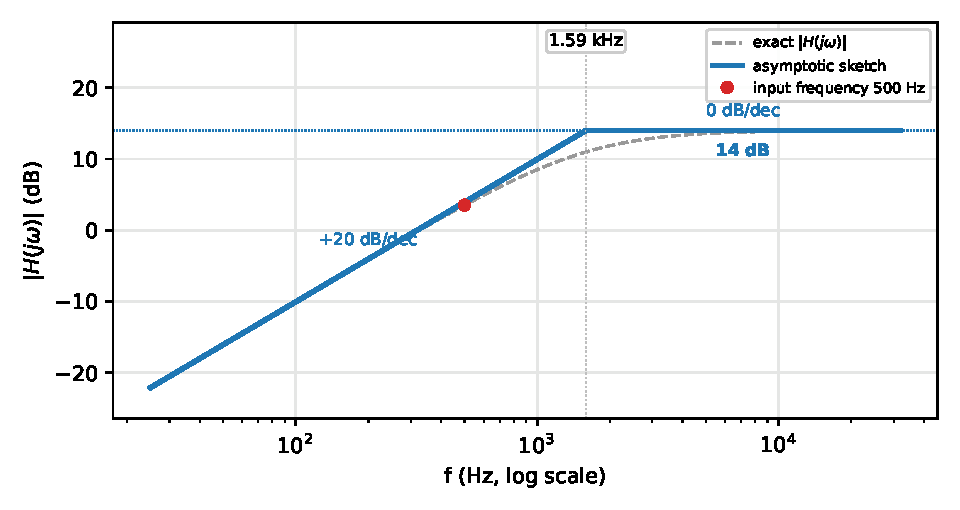
\includegraphics[width=0.78\linewidth,height=6.5cm,keepaspectratio]{p02_bode}\end{center}

{\small Blue: the straight-line sketch you are expected to draw. Dashed grey: the exact curve (about 3\,dB below the corner of an isolated pole). Red dot: the input frequency of Step 7.}
\solstep{7}{Steady-state output}The input is $V_i(t) = 0.2\sin\left(2\pi\cdot 500\,t\right)$, so $\omega_{in} = 2\pi\cdot 500 = 3140$\,rad/s. Put $s=j\omega_{in}$ in each factor (tool T5): magnitudes multiply, angles add.
{\small Rules: $\left|\frac{s}{s+p}\right| = \frac{\omega}{\sqrt{\omega^2+p^2}}$, $\angle = \frac{\pi}{2}-\tan^{-1}\frac{\omega}{p}$;\quad $\left|\frac{1}{1+s/p}\right| = \frac{1}{\sqrt{1+(\omega/p)^2}}$, $\angle = -\tan^{-1}\frac{\omega}{p}$;\quad $\left|1+\frac{s}{z}\right| = \sqrt{1+(\omega/z)^2}$, $\angle = \tan^{-1}\frac{\omega}{z}$;\quad a negative $K$ adds $-\pi$.}
\begin{center}\renewcommand{\arraystretch}{1.35}
\begin{tabular}{ccc}
\toprule
factor & magnitude & angle (rad) \\
\midrule
$-5$ & $5$ & $-3.14$ \\
$\rule[-1.1em]{0pt}{2.8em}\dfrac{s}{s+2\pi\cdot 1.59\mathrm{k}}$ & $0.2997$ & $1.27$ \\
\textbf{total} & $\mathbf{1.499}$ (product) & $\mathbf{-1.88}$ (sum) \\
\bottomrule
\end{tabular}\end{center}

\begin{align*}
|H(j\omega_{in})| &= 1.5, \qquad \angle H(j\omega_{in}) = -1.88\ \mathrm{rad} \\
v_{o,ac}(t) &= 1.5\times 0.2\,\sin\left(2\pi\cdot 500\,t - 1.88\right) = 0.3\,\sin\left(2\pi\cdot 500\,t - 1.88\right)
\end{align*}

\[
\boxed{V_o(t) = 0.3\,\sin\left(2\pi\cdot 500\,t - 1.88\right)\ \mathrm{V}}
\]

\begin{ansbox}
$H(s) = -5\,\dfrac{s}{s+2\pi\cdot 1.59\mathrm{k}}$\quad (corners: 1.59 kHz)\\[4pt]
$V_o(t) = 0.3\,\sin\left(2\pi\cdot 500\,t - 1.88\right)\ \mathrm{V}$
\end{ansbox}

\newpage
\subsection*{Solution 2B.3 \hfill Easy}
\begin{center}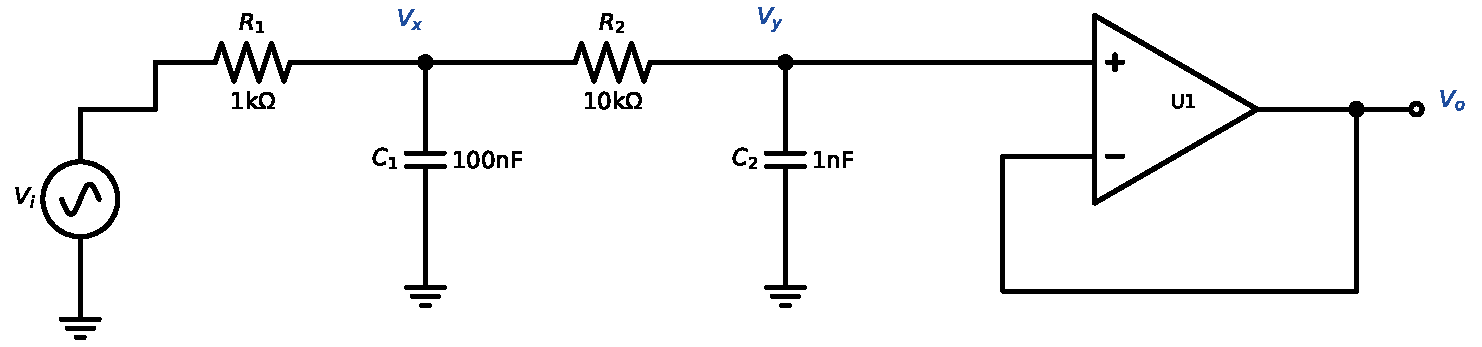
\includegraphics[width=\linewidth,height=5cm,keepaspectratio]{p03_circuit}\end{center}
\solstep{1}{Identify the sources}Independent sources: the AC input $V_i(t)$. No DC source: $V_{o,dc}=0$ and Step 2 is skipped.
\solstep{2}{DC circuit}No DC sources: $V_{o,dc}=0$.
\solstep{3}{Op-amp rules}Each op-amp has negative feedback (its output is connected back to its $-$ input), so with an ideal op-amp (tool T1): (a) no current flows into the $+$ or $-$ input; (b) $V_-=V_+$ (virtual short). The circuit is not a standard block, so it is solved by nodal analysis (tools T3, T4).
\solstep{4}{Transfer function by nodal analysis}\textbf{Block 1 (U1).} A two-section passive ladder drives the $+$ input. This is not a standard block, so use nodal analysis. Virtual short (tool T1): U1: $V_- = V_+$, so $V_{o}$ is the same voltage as $V_{y}$.
KCL (tool T3) at every node that is not an op-amp output or a source; no current flows into the op-amp inputs, so the op-amps do not appear in these sums:
\begin{align*}
&\text{(1) at }V_{x}: && \frac{V_{x} - V_{i}}{R_{1}} + sC_{1}V_{x} + \frac{V_{x} - V_{y}}{R_{2}} = 0 \\
&\text{(2) at }V_{y}: && \frac{V_{y} - V_{x}}{R_{2}} + sC_{2}V_{y} = 0
\end{align*}

Solve them one at a time (tool T4): take the equation with the fewest unknowns, solve it for one node voltage and substitute that into the remaining equations. With the component values:
\begin{align*}
\text{from (1):}\quad V_{x} &= \left(\dfrac{1000}{s + 11000}\right)V_{y} + \left(\dfrac{10000}{s + 11000}\right)V_i
\end{align*}

Substituting everything into (2) leaves only $V_{y}$ and $V_i$. Since $V_{o} = V_{y}$ (virtual short),\[
\frac{V_{o}}{V_i} = \frac{V_{y}}{V_i} = \dfrac{10^{9}}{s^{2} + 1.11\times 10^{5}\,s + 10^{9}}
\]

So:\[
H(s) = \dfrac{10^{9}}{s^{2} + 1.11\times 10^{5}\,s + 10^{9}}
\]

\solstep{5}{Standard (Bode-ready) form}Find the roots. Every root $s=-p$ of the denominator is a \emph{pole}, every root $s=-z$ of the numerator is a \emph{zero}; $|p|$ and $|z|$ are the corner frequencies (rad/s).
\begin{itemize}[leftmargin=*,itemsep=2pt]
\item Denominator: $s^{2} + 1.11\times 10^{5}\,s + 10^{9}$; quadratic formula:\[
s = \frac{-1.11\times 10^{5} \pm \sqrt{(1.11\times 10^{5})^2 - 4(10^{9})}}{2} = \frac{-1.11\times 10^{5} \pm 91200}{2} \Rightarrow s = -9890,\ -1.01\times 10^{5}
\]

\end{itemize}

Factored form (leading coefficient in front):
\[
H(s) = 10^{9}\,\dfrac{1}{(s+9890)(s+1.01\times 10^{5})}
\]

Bode-ready form: rewrite every $(s+p) = p\left(1+\frac{s}{p}\right)$ and $(s+z) = z\left(1+\frac{s}{z}\right)$, and collect all constants into $K$. Then every factor except $K$ is $\approx 1$ inside the pass-band:
\[
H(s) = 1\,\dfrac{1}{1+\dfrac{s}{2\pi\cdot 1.57\mathrm{k}}}\,\dfrac{1}{1+\dfrac{s}{2\pi\cdot 16.1\mathrm{k}}},\qquad K = 1
\]

\begin{center}\renewcommand{\arraystretch}{1.35}
\begin{tabular}{cccc}
\toprule
type & $\omega_c$ (rad/s) & $f_c=\omega_c/2\pi$ & slope change \\
\midrule
pole & $9890$ & 1.57 kHz & $-20$ dB/dec \\
pole & $1.01\times 10^{5}$ & 16.1 kHz & $-20$ dB/dec \\
\bottomrule
\end{tabular}\end{center}

\solstep{6}{Magnitude Bode plot}Below every corner, all factors are $\approx$ constant: $|H| \approx 1$ $= -0.000000000000000964$\,dB (flat, 0 dB/dec). Then, moving right, each pole bends the line down by 20\,dB/dec and each zero bends it up by 20\,dB/dec (tool T6):
\begin{center}\renewcommand{\arraystretch}{1.35}
\begin{tabular}{lcl}
\toprule
frequency range & slope & asymptote level \\
\midrule
$f<$ 1.57 kHz & $0$ dB/dec (flat) & 0 dB at end \\
1.57 kHz -- 16.1 kHz & $-20$ dB/dec & 0 dB at start, -20.2 dB at end \\
$f>$ 16.1 kHz & $-40$ dB/dec & -20.2 dB at start \\
\bottomrule
\end{tabular}\end{center}

The flat (pass-band) level is $20\log_{10}|K| = 20\log_{10}1 = -0.000000000000000964$\,dB.
\begin{center}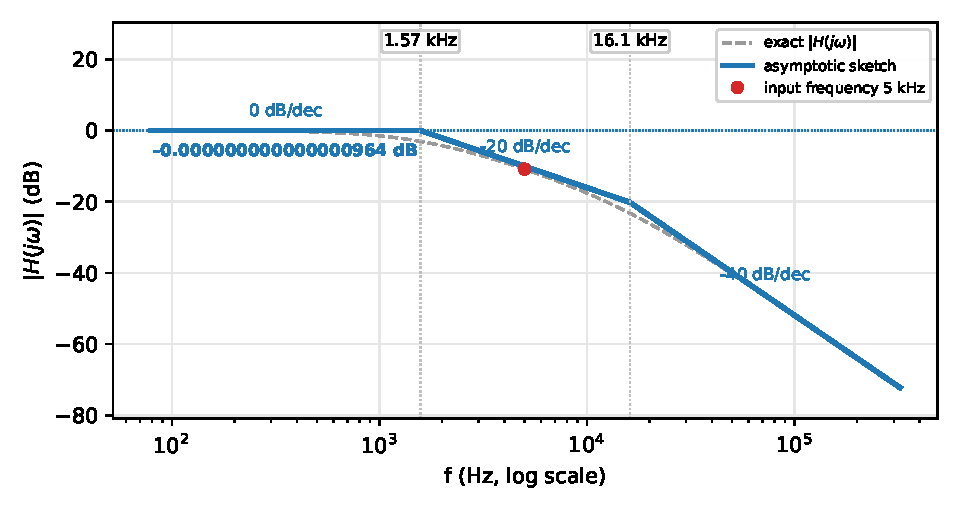
\includegraphics[width=0.78\linewidth,height=6.5cm,keepaspectratio]{p03_bode}\end{center}

{\small Blue: the straight-line sketch you are expected to draw. Dashed grey: the exact curve (about 3\,dB below the corner of an isolated pole). Red dot: the input frequency of Step 7.}
\solstep{7}{Steady-state output}The input is $V_i(t) = 1\sin\left(2\pi\cdot 5000\,t\right)$, so $\omega_{in} = 2\pi\cdot 5000 = 31400$\,rad/s. Put $s=j\omega_{in}$ in each factor (tool T5): magnitudes multiply, angles add.
{\small Rules: $\left|\frac{s}{s+p}\right| = \frac{\omega}{\sqrt{\omega^2+p^2}}$, $\angle = \frac{\pi}{2}-\tan^{-1}\frac{\omega}{p}$;\quad $\left|\frac{1}{1+s/p}\right| = \frac{1}{\sqrt{1+(\omega/p)^2}}$, $\angle = -\tan^{-1}\frac{\omega}{p}$;\quad $\left|1+\frac{s}{z}\right| = \sqrt{1+(\omega/z)^2}$, $\angle = \tan^{-1}\frac{\omega}{z}$;\quad a negative $K$ adds $-\pi$.}
\begin{center}\renewcommand{\arraystretch}{1.35}
\begin{tabular}{ccc}
\toprule
factor & magnitude & angle (rad) \\
\midrule
$1$ & $1$ & $0$ \\
$\rule[-1.7em]{0pt}{4em}\dfrac{1}{1+\dfrac{s}{2\pi\cdot 1.57\mathrm{k}}}$ & $0.3003$ & $-1.27$ \\
$\rule[-1.7em]{0pt}{4em}\dfrac{1}{1+\dfrac{s}{2\pi\cdot 16.1\mathrm{k}}}$ & $0.955$ & $-0.301$ \\
\textbf{total} & $\mathbf{0.2868}$ (product) & $\mathbf{-1.57}$ (sum) \\
\bottomrule
\end{tabular}\end{center}

\begin{align*}
|H(j\omega_{in})| &= 0.287, \qquad \angle H(j\omega_{in}) = -1.57\ \mathrm{rad} \\
v_{o,ac}(t) &= 0.287\times 1\,\sin\left(2\pi\cdot 5000\,t - 1.57\right) = 0.287\,\sin\left(2\pi\cdot 5000\,t - 1.57\right)
\end{align*}

\[
\boxed{V_o(t) = 0.287\,\sin\left(2\pi\cdot 5000\,t - 1.57\right)\ \mathrm{V}}
\]

\begin{ansbox}
$H(s) = 1\,\dfrac{1}{1+\dfrac{s}{2\pi\cdot 1.57\mathrm{k}}}\,\dfrac{1}{1+\dfrac{s}{2\pi\cdot 16.1\mathrm{k}}}$\quad (corners: 1.57 kHz, 16.1 kHz)\\[4pt]
$V_o(t) = 0.287\,\sin\left(2\pi\cdot 5000\,t - 1.57\right)\ \mathrm{V}$
\end{ansbox}

\newpage
\subsection*{Solution 2B.4 \hfill Easy}
\begin{center}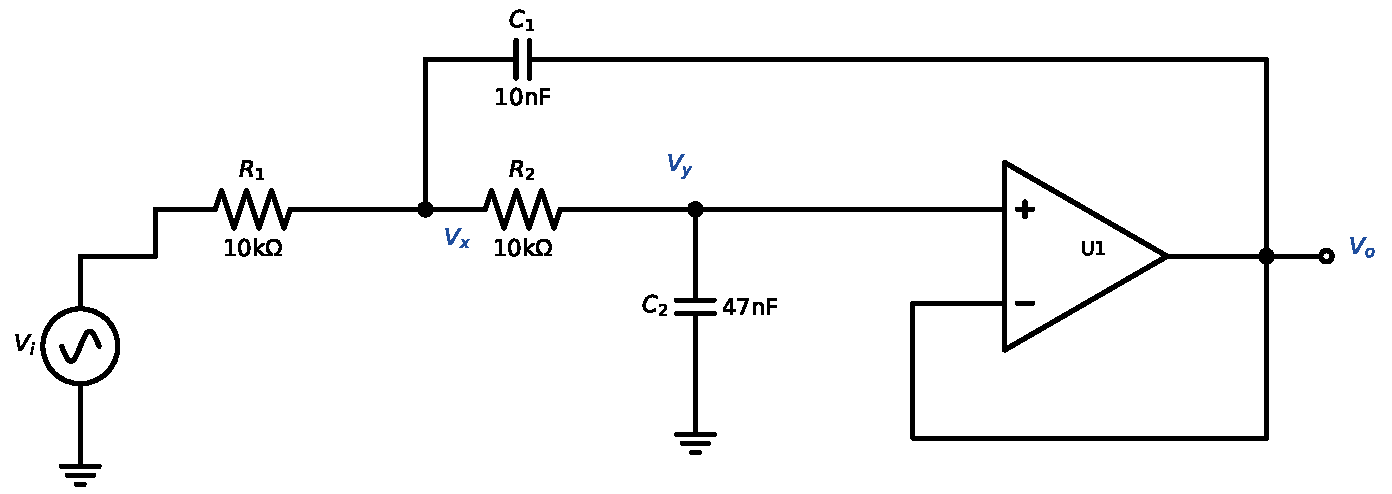
\includegraphics[width=\linewidth,height=5cm,keepaspectratio]{p04_circuit}\end{center}
\solstep{1}{Identify the sources}Independent sources: the AC input $V_i(t)$. No DC source: $V_{o,dc}=0$ and Step 2 is skipped.
\solstep{2}{DC circuit}No DC sources: $V_{o,dc}=0$.
\solstep{3}{Op-amp rules}Each op-amp has negative feedback (its output is connected back to its $-$ input), so with an ideal op-amp (tool T1): (a) no current flows into the $+$ or $-$ input; (b) $V_-=V_+$ (virtual short). The circuit is not a standard block, so it is solved by nodal analysis (tools T3, T4).
\solstep{4}{Transfer function by nodal analysis}\textbf{Block 1 (U1).} Sallen-Key stage: the network feeds back from the output to node $V_x$. This is not a standard block, so use nodal analysis. Virtual short (tool T1): U1: $V_- = V_+$, so $V_{o}$ is the same voltage as $V_{y}$.
KCL (tool T3) at every node that is not an op-amp output or a source; no current flows into the op-amp inputs, so the op-amps do not appear in these sums:
\begin{align*}
&\text{(1) at }V_{x}: && \frac{V_{x} - V_{i}}{R_{1}} + \frac{V_{x} - V_{y}}{R_{2}} + sC_{1}\left(V_{x} - V_{y}\right) = 0 \\
&\text{(2) at }V_{y}: && \frac{V_{y} - V_{x}}{R_{2}} + sC_{2}V_{y} = 0
\end{align*}

Solve them one at a time (tool T4): take the equation with the fewest unknowns, solve it for one node voltage and substitute that into the remaining equations. With the component values:
\begin{align*}
\text{from (1):}\quad V_{x} &= \left(\dfrac{s + 10000}{s + 20000}\right)V_{y} + \left(\dfrac{10000}{s + 20000}\right)V_i
\end{align*}

Substituting everything into (2) leaves only $V_{y}$ and $V_i$. Since $V_{o} = V_{y}$ (virtual short),\[
\frac{V_{o}}{V_i} = \frac{V_{y}}{V_i} = \dfrac{2.13\times 10^{7}}{s^{2} + 20000\,s + 2.13\times 10^{7}}
\]

So:\[
H(s) = \dfrac{2.13\times 10^{7}}{s^{2} + 20000\,s + 2.13\times 10^{7}}
\]

\solstep{5}{Standard (Bode-ready) form}Find the roots. Every root $s=-p$ of the denominator is a \emph{pole}, every root $s=-z$ of the numerator is a \emph{zero}; $|p|$ and $|z|$ are the corner frequencies (rad/s).
\begin{itemize}[leftmargin=*,itemsep=2pt]
\item Denominator: $s^{2} + 20000\,s + 2.13\times 10^{7}$; quadratic formula:\[
s = \frac{-20000 \pm \sqrt{(20000)^2 - 4(2.13\times 10^{7})}}{2} = \frac{-20000 \pm 17700}{2} \Rightarrow s = -1130,\ -18900
\]

\end{itemize}

Factored form (leading coefficient in front):
\[
H(s) = 2.13\times 10^{7}\,\dfrac{1}{(s+1130)(s+18900)}
\]

Bode-ready form: rewrite every $(s+p) = p\left(1+\frac{s}{p}\right)$ and $(s+z) = z\left(1+\frac{s}{z}\right)$, and collect all constants into $K$. Then every factor except $K$ is $\approx 1$ inside the pass-band:
\[
H(s) = 1\,\dfrac{1}{1+\dfrac{s}{2\pi\cdot 179}}\,\dfrac{1}{1+\dfrac{s}{2\pi\cdot 3\mathrm{k}}},\qquad K = 1
\]

\begin{center}\renewcommand{\arraystretch}{1.35}
\begin{tabular}{cccc}
\toprule
type & $\omega_c$ (rad/s) & $f_c=\omega_c/2\pi$ & slope change \\
\midrule
pole & $1130$ & 179 Hz & $-20$ dB/dec \\
pole & $18900$ & 3 kHz & $-20$ dB/dec \\
\bottomrule
\end{tabular}\end{center}

\solstep{6}{Magnitude Bode plot}Below every corner, all factors are $\approx$ constant: $|H| \approx 1$ $= 0$\,dB (flat, 0 dB/dec). Then, moving right, each pole bends the line down by 20\,dB/dec and each zero bends it up by 20\,dB/dec (tool T6):
\begin{center}\renewcommand{\arraystretch}{1.35}
\begin{tabular}{lcl}
\toprule
frequency range & slope & asymptote level \\
\midrule
$f<$ 179 Hz & $0$ dB/dec (flat) & 0 dB at end \\
179 Hz -- 3 kHz & $-20$ dB/dec & 0 dB at start, -24.5 dB at end \\
$f>$ 3 kHz & $-40$ dB/dec & -24.5 dB at start \\
\bottomrule
\end{tabular}\end{center}

The flat (pass-band) level is $20\log_{10}|K| = 20\log_{10}1 = 0$\,dB.
\begin{center}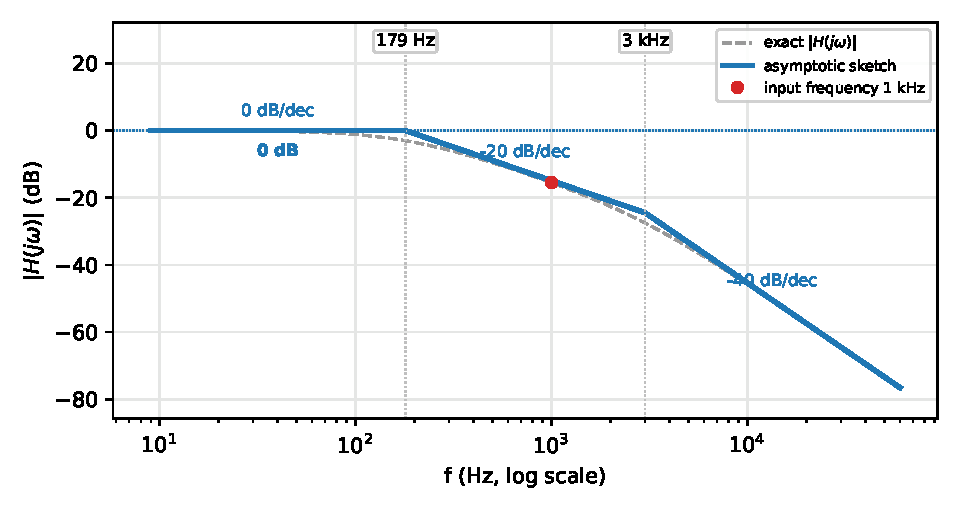
\includegraphics[width=0.78\linewidth,height=6.5cm,keepaspectratio]{p04_bode}\end{center}

{\small Blue: the straight-line sketch you are expected to draw. Dashed grey: the exact curve (about 3\,dB below the corner of an isolated pole). Red dot: the input frequency of Step 7.}
\solstep{7}{Steady-state output}The input is $V_i(t) = 0.5\sin\left(2\pi\cdot 1000\,t\right)$, so $\omega_{in} = 2\pi\cdot 1000 = 6280$\,rad/s. Put $s=j\omega_{in}$ in each factor (tool T5): magnitudes multiply, angles add.
{\small Rules: $\left|\frac{s}{s+p}\right| = \frac{\omega}{\sqrt{\omega^2+p^2}}$, $\angle = \frac{\pi}{2}-\tan^{-1}\frac{\omega}{p}$;\quad $\left|\frac{1}{1+s/p}\right| = \frac{1}{\sqrt{1+(\omega/p)^2}}$, $\angle = -\tan^{-1}\frac{\omega}{p}$;\quad $\left|1+\frac{s}{z}\right| = \sqrt{1+(\omega/z)^2}$, $\angle = \tan^{-1}\frac{\omega}{z}$;\quad a negative $K$ adds $-\pi$.}
\begin{center}\renewcommand{\arraystretch}{1.35}
\begin{tabular}{ccc}
\toprule
factor & magnitude & angle (rad) \\
\midrule
$1$ & $1$ & $0$ \\
$\rule[-1.7em]{0pt}{4em}\dfrac{1}{1+\dfrac{s}{2\pi\cdot 179}}$ & $0.1766$ & $-1.39$ \\
$\rule[-1.7em]{0pt}{4em}\dfrac{1}{1+\dfrac{s}{2\pi\cdot 3\mathrm{k}}}$ & $0.9488$ & $-0.321$ \\
\textbf{total} & $\mathbf{0.1676}$ (product) & $\mathbf{-1.71}$ (sum) \\
\bottomrule
\end{tabular}\end{center}

\begin{align*}
|H(j\omega_{in})| &= 0.168, \qquad \angle H(j\omega_{in}) = -1.71\ \mathrm{rad} \\
v_{o,ac}(t) &= 0.168\times 0.5\,\sin\left(2\pi\cdot 1000\,t - 1.71\right) = 0.0838\,\sin\left(2\pi\cdot 1000\,t - 1.71\right)
\end{align*}

\[
\boxed{V_o(t) = 0.0838\,\sin\left(2\pi\cdot 1000\,t - 1.71\right)\ \mathrm{V}}
\]

\begin{ansbox}
$H(s) = 1\,\dfrac{1}{1+\dfrac{s}{2\pi\cdot 179}}\,\dfrac{1}{1+\dfrac{s}{2\pi\cdot 3\mathrm{k}}}$\quad (corners: 179 Hz, 3 kHz)\\[4pt]
$V_o(t) = 0.0838\,\sin\left(2\pi\cdot 1000\,t - 1.71\right)\ \mathrm{V}$
\end{ansbox}

\newpage
\subsection*{Solution 2B.5 \hfill Easy}
\begin{center}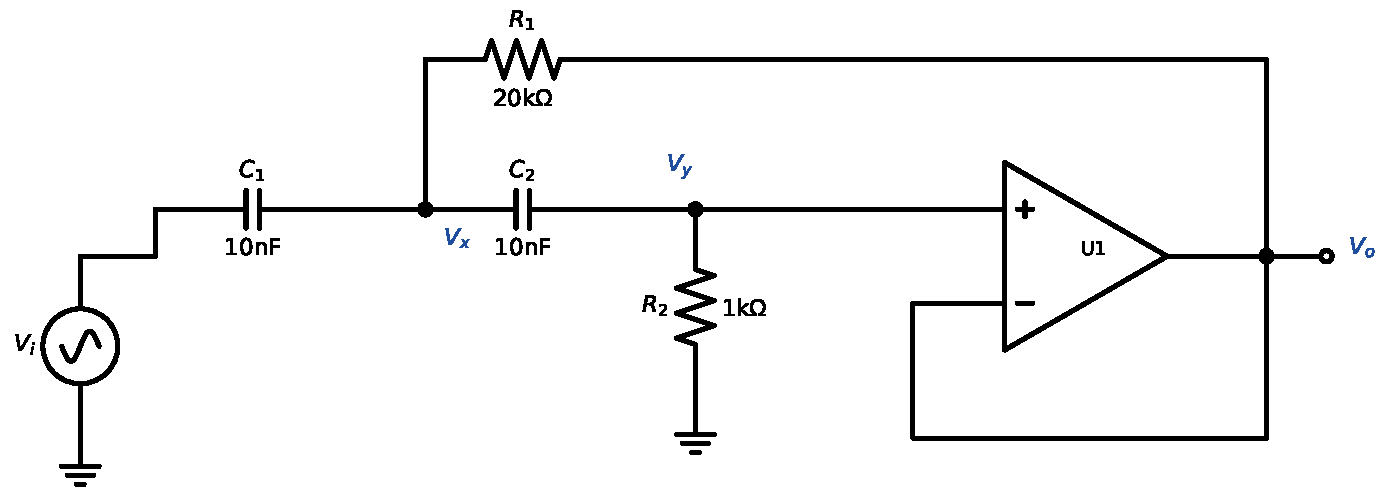
\includegraphics[width=\linewidth,height=5cm,keepaspectratio]{p05_circuit}\end{center}
\solstep{1}{Identify the sources}Independent sources: the AC input $V_i(t)$. No DC source: $V_{o,dc}=0$ and Step 2 is skipped.
\solstep{2}{DC circuit}No DC sources: $V_{o,dc}=0$.
\solstep{3}{Op-amp rules}Each op-amp has negative feedback (its output is connected back to its $-$ input), so with an ideal op-amp (tool T1): (a) no current flows into the $+$ or $-$ input; (b) $V_-=V_+$ (virtual short). The circuit is not a standard block, so it is solved by nodal analysis (tools T3, T4).
\solstep{4}{Transfer function by nodal analysis}\textbf{Block 1 (U1).} Sallen-Key stage: the network feeds back from the output to node $V_x$. This is not a standard block, so use nodal analysis. Virtual short (tool T1): U1: $V_- = V_+$, so $V_{o}$ is the same voltage as $V_{y}$.
KCL (tool T3) at every node that is not an op-amp output or a source; no current flows into the op-amp inputs, so the op-amps do not appear in these sums:
\begin{align*}
&\text{(1) at }V_{x}: && sC_{1}\left(V_{x} - V_{i}\right) + sC_{2}\left(V_{x} - V_{y}\right) + \frac{V_{x} - V_{y}}{R_{1}} = 0 \\
&\text{(2) at }V_{y}: && sC_{2}\left(V_{y} - V_{x}\right) + \frac{V_{y}}{R_{2}} = 0
\end{align*}

Solve them one at a time (tool T4): take the equation with the fewest unknowns, solve it for one node voltage and substitute that into the remaining equations. With the component values:
\begin{align*}
\text{from (1):}\quad V_{x} &= \left(\dfrac{0.5\,s + 2500}{s + 2500}\right)V_{y} + \left(\dfrac{0.5\,s}{s + 2500}\right)V_i
\end{align*}

Substituting everything into (2) leaves only $V_{y}$ and $V_i$. Since $V_{o} = V_{y}$ (virtual short),\[
\frac{V_{o}}{V_i} = \frac{V_{y}}{V_i} = \dfrac{s^{2}}{s^{2} + 2\times 10^{5}\,s + 5\times 10^{8}}
\]

So:\[
H(s) = \dfrac{s^{2}}{s^{2} + 2\times 10^{5}\,s + 5\times 10^{8}}
\]

\solstep{5}{Standard (Bode-ready) form}Find the roots. Every root $s=-p$ of the denominator is a \emph{pole}, every root $s=-z$ of the numerator is a \emph{zero}; $|p|$ and $|z|$ are the corner frequencies (rad/s).
\begin{itemize}[leftmargin=*,itemsep=2pt]
\item Numerator: it has the factor $s^2$ $\Rightarrow$ 2 zeros at $s=0$.
\item Denominator: $s^{2} + 2\times 10^{5}\,s + 5\times 10^{8}$; quadratic formula:\[
s = \frac{-2\times 10^{5} \pm \sqrt{(2\times 10^{5})^2 - 4(5\times 10^{8})}}{2} = \frac{-2\times 10^{5} \pm 1.95\times 10^{5}}{2} \Rightarrow s = -2530,\ -1.97\times 10^{5}
\]

\end{itemize}

Factored form (leading coefficient in front):
\[
H(s) = 1\,\dfrac{s^{2}}{(s+2530)(s+1.97\times 10^{5})}
\]

Bode-ready form: rewrite every $(s+p) = p\left(1+\frac{s}{p}\right)$ and $(s+z) = z\left(1+\frac{s}{z}\right)$, and collect all constants into $K$. Each $s$ in the numerator is paired with one of the \emph{lowest} poles as $\frac{s}{s+p}$ (that factor is $\approx 1$ above $p$). Then every factor except $K$ is $\approx 1$ inside the pass-band:
\[
H(s) = 1\,\dfrac{s}{s+2\pi\cdot 403}\,\dfrac{s}{s+2\pi\cdot 31.4\mathrm{k}},\qquad K = 1
\]

\begin{center}\renewcommand{\arraystretch}{1.35}
\begin{tabular}{cccc}
\toprule
type & $\omega_c$ (rad/s) & $f_c=\omega_c/2\pi$ & slope change \\
\midrule
pole & $2530$ & 403 Hz & $-20$ dB/dec \\
pole & $1.97\times 10^{5}$ & 31.4 kHz & $-20$ dB/dec \\
\bottomrule
\end{tabular}\end{center}

\solstep{6}{Magnitude Bode plot}Below every corner $|H(s)|\approx 2\times 10^{-9}\,s^2$, so the plot starts with a slope of $+40$\,dB/dec. Then, moving right, each pole bends the line down by 20\,dB/dec and each zero bends it up by 20\,dB/dec (tool T6):
\begin{center}\renewcommand{\arraystretch}{1.35}
\begin{tabular}{lcl}
\toprule
frequency range & slope & asymptote level \\
\midrule
$f<$ 403 Hz & $+40$ dB/dec & -37.8 dB at end \\
403 Hz -- 31.4 kHz & $+20$ dB/dec & -37.8 dB at start, 0 dB at end \\
$f>$ 31.4 kHz & $0$ dB/dec (flat) & 0 dB at start \\
\bottomrule
\end{tabular}\end{center}

The flat (pass-band) level is $20\log_{10}|K| = 20\log_{10}1 = 0$\,dB.
\begin{center}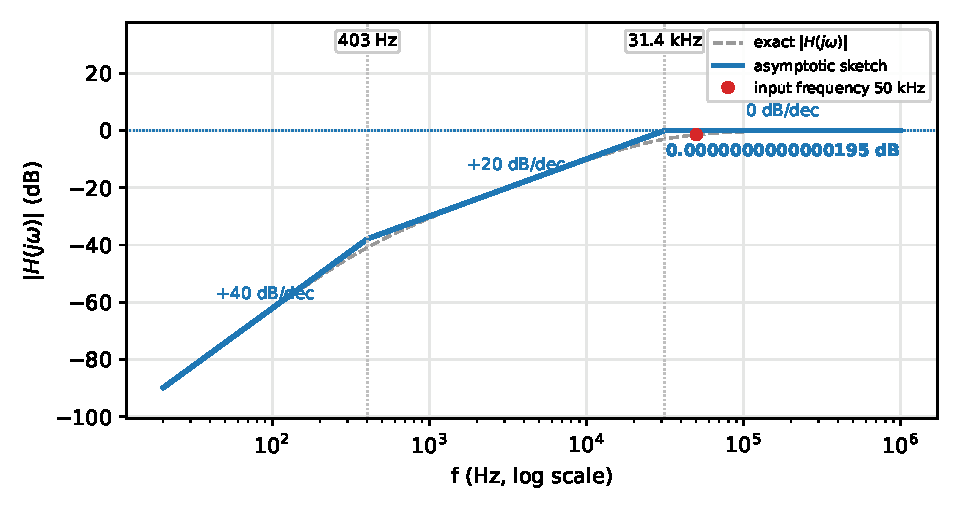
\includegraphics[width=0.78\linewidth,height=6.5cm,keepaspectratio]{p05_bode}\end{center}

{\small Blue: the straight-line sketch you are expected to draw. Dashed grey: the exact curve (about 3\,dB below the corner of an isolated pole). Red dot: the input frequency of Step 7.}
\solstep{7}{Steady-state output}The input is $V_i(t) = 0.5\sin\left(2\pi\cdot 50000\,t\right)$, so $\omega_{in} = 2\pi\cdot 50000 = 3.14\times 10^{5}$\,rad/s. Put $s=j\omega_{in}$ in each factor (tool T5): magnitudes multiply, angles add.
{\small Rules: $\left|\frac{s}{s+p}\right| = \frac{\omega}{\sqrt{\omega^2+p^2}}$, $\angle = \frac{\pi}{2}-\tan^{-1}\frac{\omega}{p}$;\quad $\left|\frac{1}{1+s/p}\right| = \frac{1}{\sqrt{1+(\omega/p)^2}}$, $\angle = -\tan^{-1}\frac{\omega}{p}$;\quad $\left|1+\frac{s}{z}\right| = \sqrt{1+(\omega/z)^2}$, $\angle = \tan^{-1}\frac{\omega}{z}$;\quad a negative $K$ adds $-\pi$.}
\begin{center}\renewcommand{\arraystretch}{1.35}
\begin{tabular}{ccc}
\toprule
factor & magnitude & angle (rad) \\
\midrule
$1$ & $1$ & $0$ \\
$\rule[-1.1em]{0pt}{2.8em}\dfrac{s}{s+2\pi\cdot 403}$ & $1$ & $0.00806$ \\
$\rule[-1.1em]{0pt}{2.8em}\dfrac{s}{s+2\pi\cdot 31.4\mathrm{k}}$ & $0.8466$ & $0.561$ \\
\textbf{total} & $\mathbf{0.8466}$ (product) & $\mathbf{0.569}$ (sum) \\
\bottomrule
\end{tabular}\end{center}

\begin{align*}
|H(j\omega_{in})| &= 0.847, \qquad \angle H(j\omega_{in}) = 0.569\ \mathrm{rad} \\
v_{o,ac}(t) &= 0.847\times 0.5\,\sin\left(2\pi\cdot 50000\,t + 0.569\right) = 0.423\,\sin\left(2\pi\cdot 50000\,t + 0.569\right)
\end{align*}

\[
\boxed{V_o(t) = 0.423\,\sin\left(2\pi\cdot 50000\,t + 0.569\right)\ \mathrm{V}}
\]

\begin{ansbox}
$H(s) = 1\,\dfrac{s}{s+2\pi\cdot 403}\,\dfrac{s}{s+2\pi\cdot 31.4\mathrm{k}}$\quad (corners: 403 Hz, 31.4 kHz)\\[4pt]
$V_o(t) = 0.423\,\sin\left(2\pi\cdot 50000\,t + 0.569\right)\ \mathrm{V}$
\end{ansbox}

\newpage
\subsection*{Solution 2B.6 \hfill Easy}
\begin{center}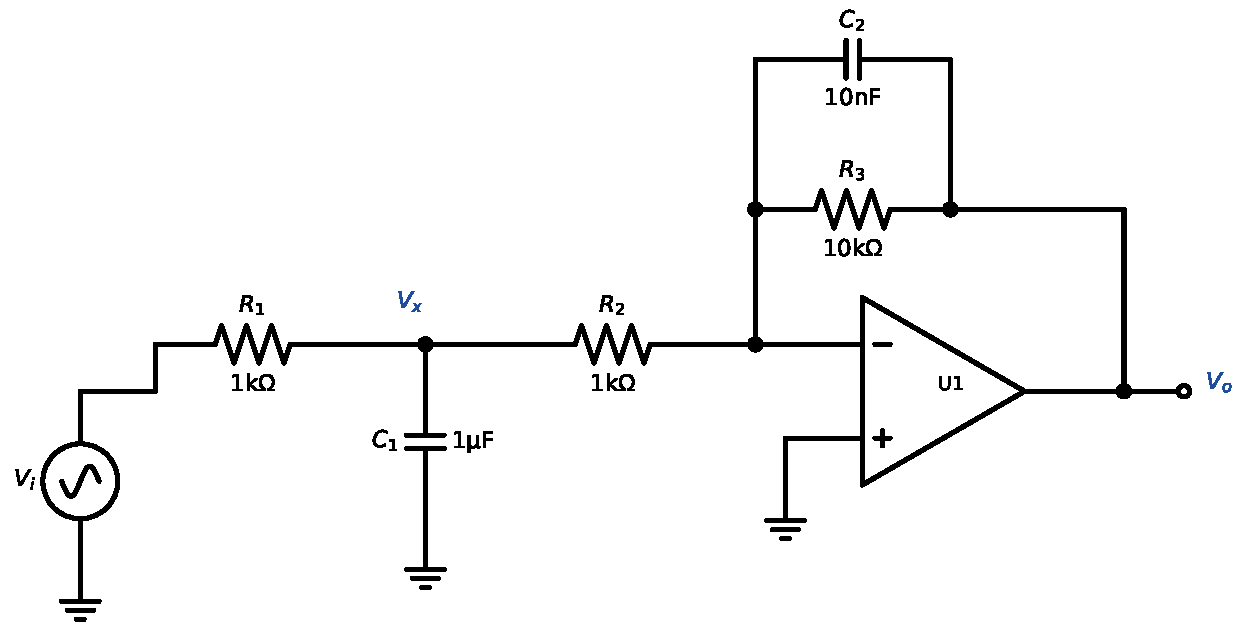
\includegraphics[width=\linewidth,height=5cm,keepaspectratio]{p06_circuit}\end{center}
\solstep{1}{Identify the sources}Independent sources: the AC input $V_i(t)$. No DC source: $V_{o,dc}=0$ and Step 2 is skipped.
\solstep{2}{DC circuit}No DC sources: $V_{o,dc}=0$.
\solstep{3}{Op-amp rules}Each op-amp has negative feedback (its output is connected back to its $-$ input), so with an ideal op-amp (tool T1): (a) no current flows into the $+$ or $-$ input; (b) $V_-=V_+$ (virtual short). The circuit is not a standard block, so it is solved by nodal analysis (tools T3, T4).
\solstep{4}{Transfer function by nodal analysis}\textbf{Block 1 (U1).} Inverting amplifier whose input network has a shunt branch. This is not a standard block, so use nodal analysis. Short names for the composite branches:\begin{align*}
Z_{f} &= R_{3} \parallel \frac{1}{sC_{2}} = \dfrac{10^{8}}{s + 10000}
\end{align*}
Virtual short (tool T1): U1: $V_- = V_+$, so $V_{-}$ is the same voltage as $0$ (virtual ground).
KCL (tool T3) at every node that is not an op-amp output or a source; no current flows into the op-amp inputs, so the op-amps do not appear in these sums:
\begin{align*}
&\text{(1) at }V_{-}\,(=0): && \frac{0 - V_{x}}{R_{2}} + \frac{0 - V_{o}}{Z_{f}} = 0 \\
&\text{(2) at }V_{x}: && \frac{V_{x} - V_{i}}{R_{1}} + sC_{1}V_{x} + \frac{V_{x}}{R_{2}} = 0
\end{align*}

Solve them one at a time (tool T4): take the equation with the fewest unknowns, solve it for one node voltage and substitute that into the remaining equations. With the component values:
\begin{align*}
\text{from (2):}\quad V_{x} &= \left(\dfrac{1000}{s + 2000}\right)V_i
\end{align*}

Substituting everything into (1) leaves only $V_{o}$ and $V_i$.\[
\frac{V_{o}}{V_i} = \dfrac{-10^{8}}{s^{2} + 12000\,s + 2\times 10^{7}}
\]

So:\[
H(s) = \dfrac{-10^{8}}{s^{2} + 12000\,s + 2\times 10^{7}}
\]

\solstep{5}{Standard (Bode-ready) form}Find the roots. Every root $s=-p$ of the denominator is a \emph{pole}, every root $s=-z$ of the numerator is a \emph{zero}; $|p|$ and $|z|$ are the corner frequencies (rad/s).
\begin{itemize}[leftmargin=*,itemsep=2pt]
\item Denominator: $s^{2} + 12000\,s + 2\times 10^{7}$; quadratic formula:\[
s = \frac{-12000 \pm \sqrt{(12000)^2 - 4(2\times 10^{7})}}{2} = \frac{-12000 \pm 8000}{2} \Rightarrow s = -2000,\ -10000
\]

\end{itemize}

Factored form (leading coefficient in front):
\[
H(s) = -10^{8}\,\dfrac{1}{(s+2000)(s+10000)}
\]

Bode-ready form: rewrite every $(s+p) = p\left(1+\frac{s}{p}\right)$ and $(s+z) = z\left(1+\frac{s}{z}\right)$, and collect all constants into $K$. Then every factor except $K$ is $\approx 1$ inside the pass-band:
\[
H(s) = -5\,\dfrac{1}{1+\dfrac{s}{2\pi\cdot 318}}\,\dfrac{1}{1+\dfrac{s}{2\pi\cdot 1.59\mathrm{k}}},\qquad K = -5
\]

\begin{center}\renewcommand{\arraystretch}{1.35}
\begin{tabular}{cccc}
\toprule
type & $\omega_c$ (rad/s) & $f_c=\omega_c/2\pi$ & slope change \\
\midrule
pole & $2000$ & 318 Hz & $-20$ dB/dec \\
pole & $10000$ & 1.59 kHz & $-20$ dB/dec \\
\bottomrule
\end{tabular}\end{center}

\solstep{6}{Magnitude Bode plot}Below every corner, all factors are $\approx$ constant: $|H| \approx 5$ $= 14$\,dB (flat, 0 dB/dec). Then, moving right, each pole bends the line down by 20\,dB/dec and each zero bends it up by 20\,dB/dec (tool T6):
\begin{center}\renewcommand{\arraystretch}{1.35}
\begin{tabular}{lcl}
\toprule
frequency range & slope & asymptote level \\
\midrule
$f<$ 318 Hz & $0$ dB/dec (flat) & 14 dB at end \\
318 Hz -- 1.59 kHz & $-20$ dB/dec & 14 dB at start, 0 dB at end \\
$f>$ 1.59 kHz & $-40$ dB/dec & 0 dB at start \\
\bottomrule
\end{tabular}\end{center}

The flat (pass-band) level is $20\log_{10}|K| = 20\log_{10}5 = 14$\,dB.
\begin{center}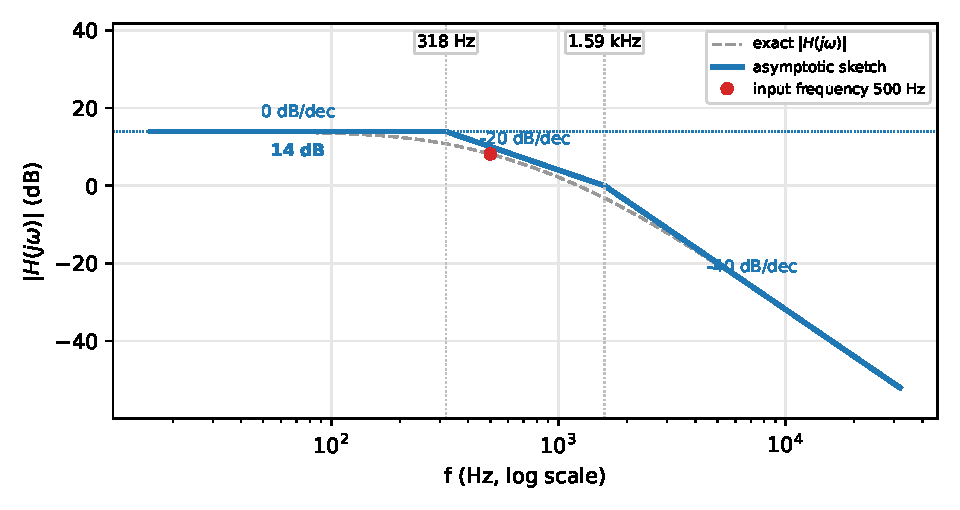
\includegraphics[width=0.78\linewidth,height=6.5cm,keepaspectratio]{p06_bode}\end{center}

{\small Blue: the straight-line sketch you are expected to draw. Dashed grey: the exact curve (about 3\,dB below the corner of an isolated pole). Red dot: the input frequency of Step 7.}
\solstep{7}{Steady-state output}The input is $V_i(t) = 0.1\cos\left(2\pi\cdot 500\,t\right)$, so $\omega_{in} = 2\pi\cdot 500 = 3140$\,rad/s. Put $s=j\omega_{in}$ in each factor (tool T5): magnitudes multiply, angles add.
{\small Rules: $\left|\frac{s}{s+p}\right| = \frac{\omega}{\sqrt{\omega^2+p^2}}$, $\angle = \frac{\pi}{2}-\tan^{-1}\frac{\omega}{p}$;\quad $\left|\frac{1}{1+s/p}\right| = \frac{1}{\sqrt{1+(\omega/p)^2}}$, $\angle = -\tan^{-1}\frac{\omega}{p}$;\quad $\left|1+\frac{s}{z}\right| = \sqrt{1+(\omega/z)^2}$, $\angle = \tan^{-1}\frac{\omega}{z}$;\quad a negative $K$ adds $-\pi$.}
\begin{center}\renewcommand{\arraystretch}{1.35}
\begin{tabular}{ccc}
\toprule
factor & magnitude & angle (rad) \\
\midrule
$-5$ & $5$ & $-3.14$ \\
$\rule[-1.7em]{0pt}{4em}\dfrac{1}{1+\dfrac{s}{2\pi\cdot 318}}$ & $0.537$ & $-1$ \\
$\rule[-1.7em]{0pt}{4em}\dfrac{1}{1+\dfrac{s}{2\pi\cdot 1.59\mathrm{k}}}$ & $0.954$ & $-0.304$ \\
\textbf{total} & $\mathbf{2.562}$ (product) & $\mathbf{-4.45}$ (sum) \\
\bottomrule
\end{tabular}\end{center}

\begin{align*}
|H(j\omega_{in})| &= 2.56, \qquad \angle H(j\omega_{in}) = -4.45\ \mathrm{rad} \\
v_{o,ac}(t) &= 2.56\times 0.1\,\cos\left(2\pi\cdot 500\,t - 4.45\right) = 0.256\,\cos\left(2\pi\cdot 500\,t - 4.45\right)
\end{align*}

\[
\boxed{V_o(t) = 0.256\,\cos\left(2\pi\cdot 500\,t - 4.45\right)\ \mathrm{V}}
\]

\begin{ansbox}
$H(s) = -5\,\dfrac{1}{1+\dfrac{s}{2\pi\cdot 318}}\,\dfrac{1}{1+\dfrac{s}{2\pi\cdot 1.59\mathrm{k}}}$\quad (corners: 318 Hz, 1.59 kHz)\\[4pt]
$V_o(t) = 0.256\,\cos\left(2\pi\cdot 500\,t - 4.45\right)\ \mathrm{V}$
\end{ansbox}

\newpage
\subsection*{Solution 2B.7 \hfill Medium}
\begin{center}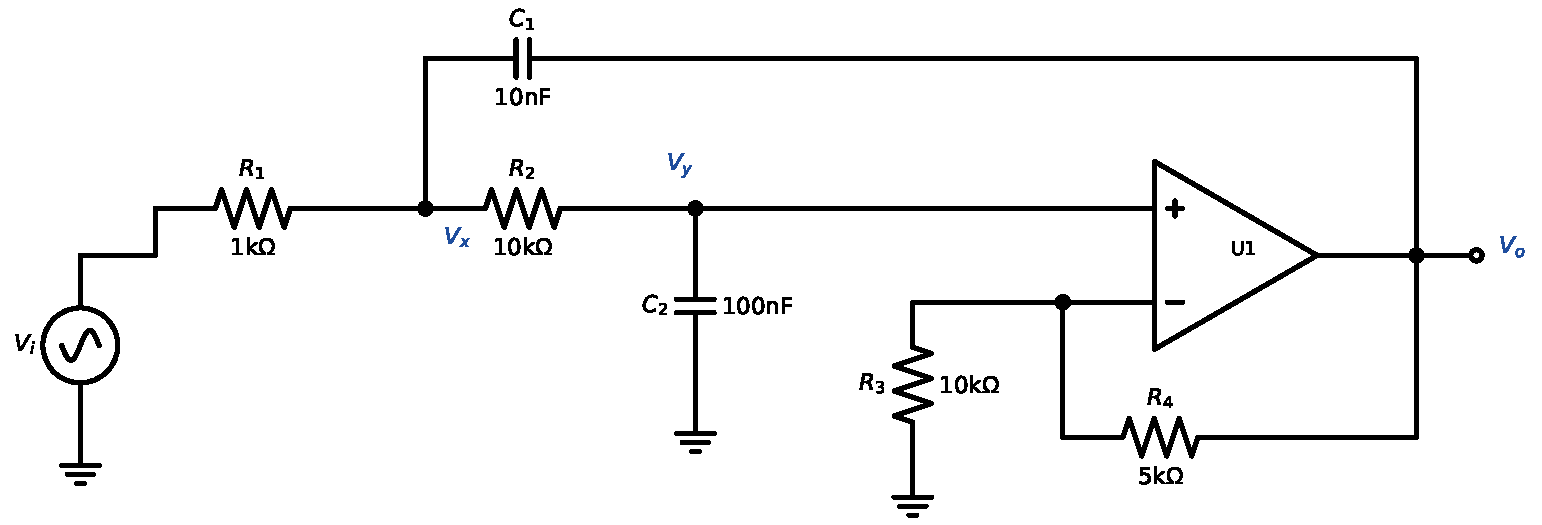
\includegraphics[width=\linewidth,height=5cm,keepaspectratio]{p07_circuit}\end{center}
\solstep{1}{Identify the sources}Independent sources: the AC input $V_i(t)$. No DC source: $V_{o,dc}=0$ and Step 2 is skipped.
\solstep{2}{DC circuit}No DC sources: $V_{o,dc}=0$.
\solstep{3}{Op-amp rules}Each op-amp has negative feedback (its output is connected back to its $-$ input), so with an ideal op-amp (tool T1): (a) no current flows into the $+$ or $-$ input; (b) $V_-=V_+$ (virtual short). The circuit is not a standard block, so it is solved by nodal analysis (tools T3, T4).
\solstep{4}{Transfer function by nodal analysis}\textbf{Block 1 (U1).} Sallen-Key stage: the network feeds back from the output to node $V_x$. This is not a standard block, so use nodal analysis. Virtual short (tool T1): U1: $V_- = V_+$, so $V_{-}$ is the same voltage as $V_{y}$.
KCL (tool T3) at every node that is not an op-amp output or a source; no current flows into the op-amp inputs, so the op-amps do not appear in these sums:
\begin{align*}
&\text{(1) at }V_{-}\,(=V_{y}): && \frac{V_{y}}{R_{3}} + \frac{V_{y} - V_{o}}{R_{4}} = 0 \\
&\text{(2) at }V_{x}: && \frac{V_{x} - V_{i}}{R_{1}} + \frac{V_{x} - V_{y}}{R_{2}} + sC_{1}\left(V_{x} - V_{o}\right) = 0 \\
&\text{(3) at }V_{y}: && \frac{V_{y} - V_{x}}{R_{2}} + sC_{2}V_{y} = 0
\end{align*}

Solve them one at a time (tool T4): take the equation with the fewest unknowns, solve it for one node voltage and substitute that into the remaining equations. With the component values:
\begin{align*}
\text{from (1):}\quad V_{y} &= 0.667\,V_{o} \\
\text{from (2):}\quad V_{x} &= \left(\dfrac{s + 6670}{s + 1.1\times 10^{5}}\right)V_{o} + \left(\dfrac{10^{5}}{s + 1.1\times 10^{5}}\right)V_i
\end{align*}

Substituting everything into (3) leaves only $V_{o}$ and $V_i$.\[
\frac{V_{o}}{V_i} = \dfrac{1.5\times 10^{8}}{s^{2} + 1.09\times 10^{5}\,s + 10^{8}}
\]

So:\[
H(s) = \dfrac{1.5\times 10^{8}}{s^{2} + 1.09\times 10^{5}\,s + 10^{8}}
\]

\solstep{5}{Standard (Bode-ready) form}Find the roots. Every root $s=-p$ of the denominator is a \emph{pole}, every root $s=-z$ of the numerator is a \emph{zero}; $|p|$ and $|z|$ are the corner frequencies (rad/s).
\begin{itemize}[leftmargin=*,itemsep=2pt]
\item Denominator: $s^{2} + 1.09\times 10^{5}\,s + 10^{8}$; quadratic formula:\[
s = \frac{-1.09\times 10^{5} \pm \sqrt{(1.09\times 10^{5})^2 - 4(10^{8})}}{2} = \frac{-1.09\times 10^{5} \pm 1.08\times 10^{5}}{2} \Rightarrow s = -921,\ -1.09\times 10^{5}
\]

\end{itemize}

Factored form (leading coefficient in front):
\[
H(s) = 1.5\times 10^{8}\,\dfrac{1}{(s+921)(s+1.09\times 10^{5})}
\]

Bode-ready form: rewrite every $(s+p) = p\left(1+\frac{s}{p}\right)$ and $(s+z) = z\left(1+\frac{s}{z}\right)$, and collect all constants into $K$. Then every factor except $K$ is $\approx 1$ inside the pass-band:
\[
H(s) = 1.5\,\dfrac{1}{1+\dfrac{s}{2\pi\cdot 147}}\,\dfrac{1}{1+\dfrac{s}{2\pi\cdot 17.3\mathrm{k}}},\qquad K = 1.5
\]

\begin{center}\renewcommand{\arraystretch}{1.35}
\begin{tabular}{cccc}
\toprule
type & $\omega_c$ (rad/s) & $f_c=\omega_c/2\pi$ & slope change \\
\midrule
pole & $921$ & 147 Hz & $-20$ dB/dec \\
pole & $1.09\times 10^{5}$ & 17.3 kHz & $-20$ dB/dec \\
\bottomrule
\end{tabular}\end{center}

\solstep{6}{Magnitude Bode plot}Below every corner, all factors are $\approx$ constant: $|H| \approx 1.5$ $= 3.52$\,dB (flat, 0 dB/dec). Then, moving right, each pole bends the line down by 20\,dB/dec and each zero bends it up by 20\,dB/dec (tool T6):
\begin{center}\renewcommand{\arraystretch}{1.35}
\begin{tabular}{lcl}
\toprule
frequency range & slope & asymptote level \\
\midrule
$f<$ 147 Hz & $0$ dB/dec (flat) & 3.52 dB at end \\
147 Hz -- 17.3 kHz & $-20$ dB/dec & 3.52 dB at start, -37.9 dB at end \\
$f>$ 17.3 kHz & $-40$ dB/dec & -37.9 dB at start \\
\bottomrule
\end{tabular}\end{center}

The flat (pass-band) level is $20\log_{10}|K| = 20\log_{10}1.5 = 3.52$\,dB.
\begin{center}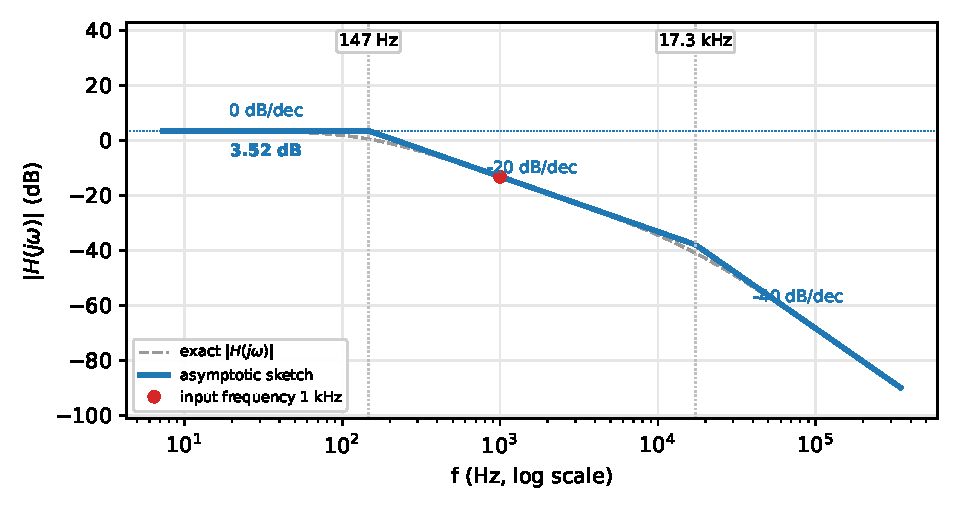
\includegraphics[width=0.78\linewidth,height=6.5cm,keepaspectratio]{p07_bode}\end{center}

{\small Blue: the straight-line sketch you are expected to draw. Dashed grey: the exact curve (about 3\,dB below the corner of an isolated pole). Red dot: the input frequency of Step 7.}
\solstep{7}{Steady-state output}The input is $V_i(t) = 0.2\sin\left(2\pi\cdot 1000\,t\right)$, so $\omega_{in} = 2\pi\cdot 1000 = 6280$\,rad/s. Put $s=j\omega_{in}$ in each factor (tool T5): magnitudes multiply, angles add.
{\small Rules: $\left|\frac{s}{s+p}\right| = \frac{\omega}{\sqrt{\omega^2+p^2}}$, $\angle = \frac{\pi}{2}-\tan^{-1}\frac{\omega}{p}$;\quad $\left|\frac{1}{1+s/p}\right| = \frac{1}{\sqrt{1+(\omega/p)^2}}$, $\angle = -\tan^{-1}\frac{\omega}{p}$;\quad $\left|1+\frac{s}{z}\right| = \sqrt{1+(\omega/z)^2}$, $\angle = \tan^{-1}\frac{\omega}{z}$;\quad a negative $K$ adds $-\pi$.}
\begin{center}\renewcommand{\arraystretch}{1.35}
\begin{tabular}{ccc}
\toprule
factor & magnitude & angle (rad) \\
\midrule
$1.5$ & $1.5$ & $0$ \\
$\rule[-1.7em]{0pt}{4em}\dfrac{1}{1+\dfrac{s}{2\pi\cdot 147}}$ & $0.145$ & $-1.43$ \\
$\rule[-1.7em]{0pt}{4em}\dfrac{1}{1+\dfrac{s}{2\pi\cdot 17.3\mathrm{k}}}$ & $0.9983$ & $-0.0578$ \\
\textbf{total} & $\mathbf{0.2172}$ (product) & $\mathbf{-1.48}$ (sum) \\
\bottomrule
\end{tabular}\end{center}

\begin{align*}
|H(j\omega_{in})| &= 0.217, \qquad \angle H(j\omega_{in}) = -1.48\ \mathrm{rad} \\
v_{o,ac}(t) &= 0.217\times 0.2\,\sin\left(2\pi\cdot 1000\,t - 1.48\right) = 0.0434\,\sin\left(2\pi\cdot 1000\,t - 1.48\right)
\end{align*}

\[
\boxed{V_o(t) = 0.0434\,\sin\left(2\pi\cdot 1000\,t - 1.48\right)\ \mathrm{V}}
\]

\begin{ansbox}
$H(s) = 1.5\,\dfrac{1}{1+\dfrac{s}{2\pi\cdot 147}}\,\dfrac{1}{1+\dfrac{s}{2\pi\cdot 17.3\mathrm{k}}}$\quad (corners: 147 Hz, 17.3 kHz)\\[4pt]
$V_o(t) = 0.0434\,\sin\left(2\pi\cdot 1000\,t - 1.48\right)\ \mathrm{V}$
\end{ansbox}

\newpage
\subsection*{Solution 2B.8 \hfill Medium}
\begin{center}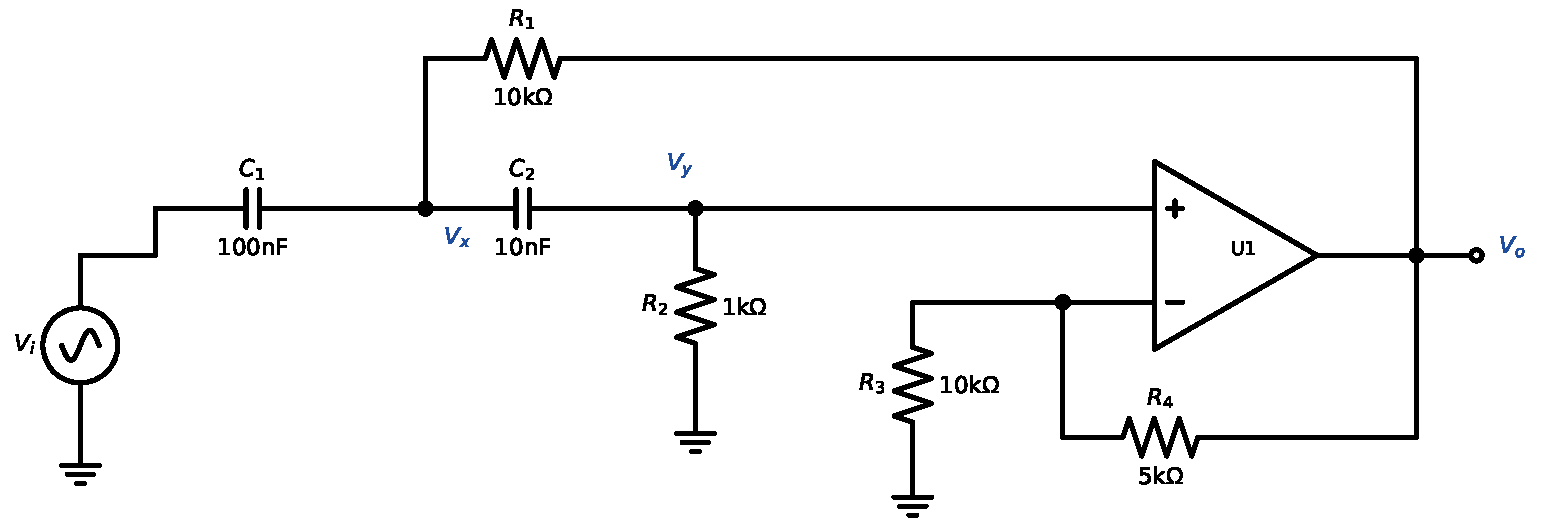
\includegraphics[width=\linewidth,height=5cm,keepaspectratio]{p08_circuit}\end{center}
\solstep{1}{Identify the sources}Independent sources: the AC input $V_i(t)$. No DC source: $V_{o,dc}=0$ and Step 2 is skipped.
\solstep{2}{DC circuit}No DC sources: $V_{o,dc}=0$.
\solstep{3}{Op-amp rules}Each op-amp has negative feedback (its output is connected back to its $-$ input), so with an ideal op-amp (tool T1): (a) no current flows into the $+$ or $-$ input; (b) $V_-=V_+$ (virtual short). The circuit is not a standard block, so it is solved by nodal analysis (tools T3, T4).
\solstep{4}{Transfer function by nodal analysis}\textbf{Block 1 (U1).} Sallen-Key stage: the network feeds back from the output to node $V_x$. This is not a standard block, so use nodal analysis. Virtual short (tool T1): U1: $V_- = V_+$, so $V_{-}$ is the same voltage as $V_{y}$.
KCL (tool T3) at every node that is not an op-amp output or a source; no current flows into the op-amp inputs, so the op-amps do not appear in these sums:
\begin{align*}
&\text{(1) at }V_{-}\,(=V_{y}): && \frac{V_{y}}{R_{3}} + \frac{V_{y} - V_{o}}{R_{4}} = 0 \\
&\text{(2) at }V_{x}: && sC_{1}\left(V_{x} - V_{i}\right) + sC_{2}\left(V_{x} - V_{y}\right) + \frac{V_{x} - V_{o}}{R_{1}} = 0 \\
&\text{(3) at }V_{y}: && sC_{2}\left(V_{y} - V_{x}\right) + \frac{V_{y}}{R_{2}} = 0
\end{align*}

Solve them one at a time (tool T4): take the equation with the fewest unknowns, solve it for one node voltage and substitute that into the remaining equations. With the component values:
\begin{align*}
\text{from (1):}\quad V_{y} &= 0.667\,V_{o} \\
\text{from (2):}\quad V_{x} &= \left(\dfrac{0.0606\,s + 909}{s + 909}\right)V_{o} + \left(\dfrac{0.909\,s}{s + 909}\right)V_i
\end{align*}

Substituting everything into (3) leaves only $V_{o}$ and $V_i$.\[
\frac{V_{o}}{V_i} = \dfrac{1.5\,s^{2}}{s^{2} + 1.09\times 10^{5}\,s + 10^{8}}
\]

So:\[
H(s) = \dfrac{1.5\,s^{2}}{s^{2} + 1.09\times 10^{5}\,s + 10^{8}}
\]

\solstep{5}{Standard (Bode-ready) form}Find the roots. Every root $s=-p$ of the denominator is a \emph{pole}, every root $s=-z$ of the numerator is a \emph{zero}; $|p|$ and $|z|$ are the corner frequencies (rad/s).
\begin{itemize}[leftmargin=*,itemsep=2pt]
\item Numerator: it has the factor $s^2$ $\Rightarrow$ 2 zeros at $s=0$.
\item Denominator: $s^{2} + 1.09\times 10^{5}\,s + 10^{8}$; quadratic formula:\[
s = \frac{-1.09\times 10^{5} \pm \sqrt{(1.09\times 10^{5})^2 - 4(10^{8})}}{2} = \frac{-1.09\times 10^{5} \pm 1.08\times 10^{5}}{2} \Rightarrow s = -921,\ -1.09\times 10^{5}
\]

\end{itemize}

Factored form (leading coefficient in front):
\[
H(s) = 1.5\,\dfrac{s^{2}}{(s+921)(s+1.09\times 10^{5})}
\]

Bode-ready form: rewrite every $(s+p) = p\left(1+\frac{s}{p}\right)$ and $(s+z) = z\left(1+\frac{s}{z}\right)$, and collect all constants into $K$. Each $s$ in the numerator is paired with one of the \emph{lowest} poles as $\frac{s}{s+p}$ (that factor is $\approx 1$ above $p$). Then every factor except $K$ is $\approx 1$ inside the pass-band:
\[
H(s) = 1.5\,\dfrac{s}{s+2\pi\cdot 147}\,\dfrac{s}{s+2\pi\cdot 17.3\mathrm{k}},\qquad K = 1.5
\]

\begin{center}\renewcommand{\arraystretch}{1.35}
\begin{tabular}{cccc}
\toprule
type & $\omega_c$ (rad/s) & $f_c=\omega_c/2\pi$ & slope change \\
\midrule
pole & $921$ & 147 Hz & $-20$ dB/dec \\
pole & $1.09\times 10^{5}$ & 17.3 kHz & $-20$ dB/dec \\
\bottomrule
\end{tabular}\end{center}

\solstep{6}{Magnitude Bode plot}Below every corner $|H(s)|\approx 1.5\times 10^{-8}\,s^2$, so the plot starts with a slope of $+40$\,dB/dec. Then, moving right, each pole bends the line down by 20\,dB/dec and each zero bends it up by 20\,dB/dec (tool T6):
\begin{center}\renewcommand{\arraystretch}{1.35}
\begin{tabular}{lcl}
\toprule
frequency range & slope & asymptote level \\
\midrule
$f<$ 147 Hz & $+40$ dB/dec & -37.9 dB at end \\
147 Hz -- 17.3 kHz & $+20$ dB/dec & -37.9 dB at start, 3.52 dB at end \\
$f>$ 17.3 kHz & $0$ dB/dec (flat) & 3.52 dB at start \\
\bottomrule
\end{tabular}\end{center}

The flat (pass-band) level is $20\log_{10}|K| = 20\log_{10}1.5 = 3.52$\,dB.
\begin{center}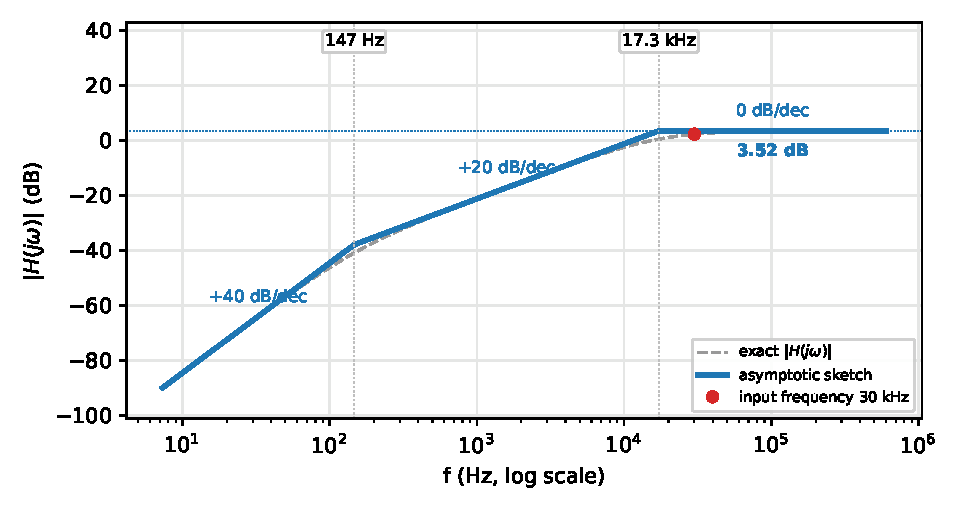
\includegraphics[width=0.78\linewidth,height=6.5cm,keepaspectratio]{p08_bode}\end{center}

{\small Blue: the straight-line sketch you are expected to draw. Dashed grey: the exact curve (about 3\,dB below the corner of an isolated pole). Red dot: the input frequency of Step 7.}
\solstep{7}{Steady-state output}The input is $V_i(t) = 0.2\sin\left(2\pi\cdot 30000\,t\right)$, so $\omega_{in} = 2\pi\cdot 30000 = 1.88\times 10^{5}$\,rad/s. Put $s=j\omega_{in}$ in each factor (tool T5): magnitudes multiply, angles add.
{\small Rules: $\left|\frac{s}{s+p}\right| = \frac{\omega}{\sqrt{\omega^2+p^2}}$, $\angle = \frac{\pi}{2}-\tan^{-1}\frac{\omega}{p}$;\quad $\left|\frac{1}{1+s/p}\right| = \frac{1}{\sqrt{1+(\omega/p)^2}}$, $\angle = -\tan^{-1}\frac{\omega}{p}$;\quad $\left|1+\frac{s}{z}\right| = \sqrt{1+(\omega/z)^2}$, $\angle = \tan^{-1}\frac{\omega}{z}$;\quad a negative $K$ adds $-\pi$.}
\begin{center}\renewcommand{\arraystretch}{1.35}
\begin{tabular}{ccc}
\toprule
factor & magnitude & angle (rad) \\
\midrule
$1.5$ & $1.5$ & $0$ \\
$\rule[-1.1em]{0pt}{2.8em}\dfrac{s}{s+2\pi\cdot 147}$ & $1$ & $0.00489$ \\
$\rule[-1.1em]{0pt}{2.8em}\dfrac{s}{s+2\pi\cdot 17.3\mathrm{k}}$ & $0.8665$ & $0.523$ \\
\textbf{total} & $\mathbf{1.3}$ (product) & $\mathbf{0.527}$ (sum) \\
\bottomrule
\end{tabular}\end{center}

\begin{align*}
|H(j\omega_{in})| &= 1.3, \qquad \angle H(j\omega_{in}) = 0.527\ \mathrm{rad} \\
v_{o,ac}(t) &= 1.3\times 0.2\,\sin\left(2\pi\cdot 30000\,t + 0.527\right) = 0.26\,\sin\left(2\pi\cdot 30000\,t + 0.527\right)
\end{align*}

\[
\boxed{V_o(t) = 0.26\,\sin\left(2\pi\cdot 30000\,t + 0.527\right)\ \mathrm{V}}
\]

\begin{ansbox}
$H(s) = 1.5\,\dfrac{s}{s+2\pi\cdot 147}\,\dfrac{s}{s+2\pi\cdot 17.3\mathrm{k}}$\quad (corners: 147 Hz, 17.3 kHz)\\[4pt]
$V_o(t) = 0.26\,\sin\left(2\pi\cdot 30000\,t + 0.527\right)\ \mathrm{V}$
\end{ansbox}

\newpage
\subsection*{Solution 2B.9 \hfill Medium}
\begin{center}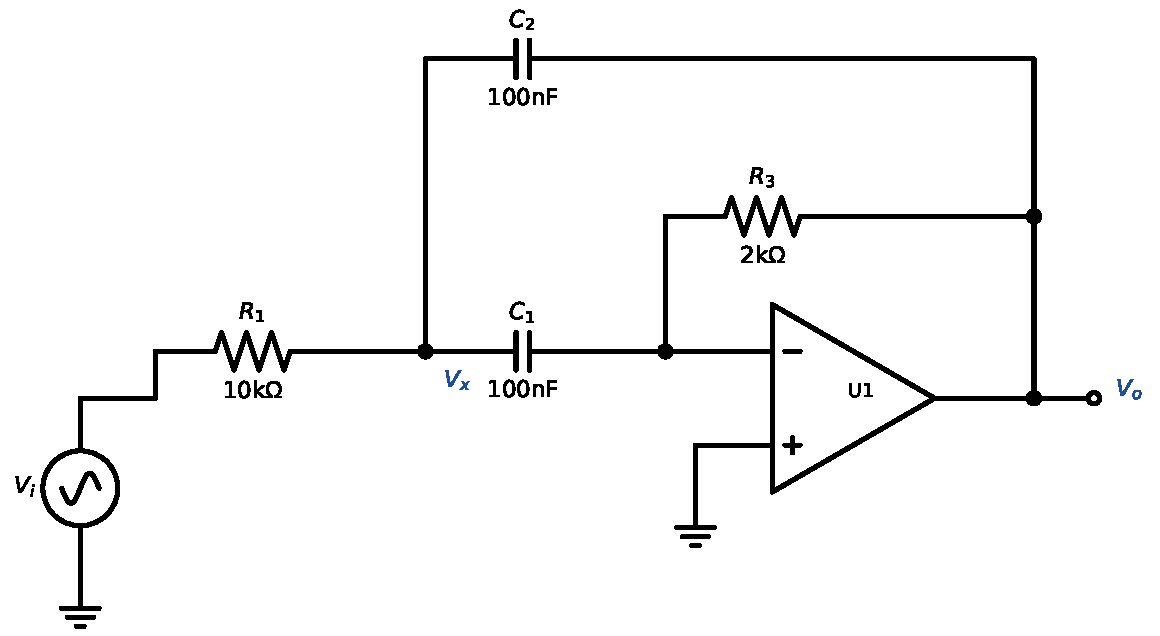
\includegraphics[width=\linewidth,height=5cm,keepaspectratio]{p09_circuit}\end{center}
\solstep{1}{Identify the sources}Independent sources: the AC input $V_i(t)$. No DC source: $V_{o,dc}=0$ and Step 2 is skipped.
\solstep{2}{DC circuit}No DC sources: $V_{o,dc}=0$.
\solstep{3}{Op-amp rules}Each op-amp has negative feedback (its output is connected back to its $-$ input), so with an ideal op-amp (tool T1): (a) no current flows into the $+$ or $-$ input; (b) $V_-=V_+$ (virtual short). The circuit is not a standard block, so it is solved by nodal analysis (tools T3, T4).
\solstep{4}{Transfer function by nodal analysis}\textbf{Block 1 (U1).} Multiple-feedback stage: node $V_x$ is fed back from the output through a second branch. This is not a standard block, so use nodal analysis. Virtual short (tool T1): U1: $V_- = V_+$, so $V_{-}$ is the same voltage as $0$ (virtual ground).
KCL (tool T3) at every node that is not an op-amp output or a source; no current flows into the op-amp inputs, so the op-amps do not appear in these sums:
\begin{align*}
&\text{(1) at }V_{-}\,(=0): && sC_{1}\left(0 - V_{x}\right) + \frac{0 - V_{o}}{R_{3}} = 0 \\
&\text{(2) at }V_{x}: && \frac{V_{x} - V_{i}}{R_{1}} + sC_{1}V_{x} + sC_{2}\left(V_{x} - V_{o}\right) = 0
\end{align*}

Solve them one at a time (tool T4): take the equation with the fewest unknowns, solve it for one node voltage and substitute that into the remaining equations. With the component values:
\begin{align*}
\text{from (1):}\quad V_{x} &= \left(\dfrac{-5000}{s}\right)V_{o}
\end{align*}

Substituting everything into (2) leaves only $V_{o}$ and $V_i$.\[
\frac{V_{o}}{V_i} = \dfrac{-1000\,s}{s^{2} + 10000\,s + 5\times 10^{6}}
\]

So:\[
H(s) = \dfrac{-1000\,s}{s^{2} + 10000\,s + 5\times 10^{6}}
\]

\solstep{5}{Standard (Bode-ready) form}Find the roots. Every root $s=-p$ of the denominator is a \emph{pole}, every root $s=-z$ of the numerator is a \emph{zero}; $|p|$ and $|z|$ are the corner frequencies (rad/s).
\begin{itemize}[leftmargin=*,itemsep=2pt]
\item Numerator: it has the factor $s$ $\Rightarrow$ 1 zero at $s=0$.
\item Denominator: $s^{2} + 10000\,s + 5\times 10^{6}$; quadratic formula:\[
s = \frac{-10000 \pm \sqrt{(10000)^2 - 4(5\times 10^{6})}}{2} = \frac{-10000 \pm 8940}{2} \Rightarrow s = -528,\ -9470
\]

\end{itemize}

Factored form (leading coefficient in front):
\[
H(s) = -1000\,\dfrac{s}{(s+528)(s+9470)}
\]

Bode-ready form: rewrite every $(s+p) = p\left(1+\frac{s}{p}\right)$ and $(s+z) = z\left(1+\frac{s}{z}\right)$, and collect all constants into $K$. Each $s$ in the numerator is paired with one of the \emph{lowest} poles as $\frac{s}{s+p}$ (that factor is $\approx 1$ above $p$). Then every factor except $K$ is $\approx 1$ inside the pass-band:
\[
H(s) = -0.106\,\dfrac{s}{s+2\pi\cdot 84}\,\dfrac{1}{1+\dfrac{s}{2\pi\cdot 1.51\mathrm{k}}},\qquad K = -0.106
\]

\begin{center}\renewcommand{\arraystretch}{1.35}
\begin{tabular}{cccc}
\toprule
type & $\omega_c$ (rad/s) & $f_c=\omega_c/2\pi$ & slope change \\
\midrule
pole & $528$ & 84 Hz & $-20$ dB/dec \\
pole & $9470$ & 1.51 kHz & $-20$ dB/dec \\
\bottomrule
\end{tabular}\end{center}

\solstep{6}{Magnitude Bode plot}Below every corner $|H(s)|\approx 2\times 10^{-4}\,s$, so the plot starts with a slope of $+20$\,dB/dec. Then, moving right, each pole bends the line down by 20\,dB/dec and each zero bends it up by 20\,dB/dec (tool T6):
\begin{center}\renewcommand{\arraystretch}{1.35}
\begin{tabular}{lcl}
\toprule
frequency range & slope & asymptote level \\
\midrule
$f<$ 84 Hz & $+20$ dB/dec & -19.5 dB at end \\
84 Hz -- 1.51 kHz & $0$ dB/dec (flat) & -19.5 dB at start, -19.5 dB at end \\
$f>$ 1.51 kHz & $-20$ dB/dec & -19.5 dB at start \\
\bottomrule
\end{tabular}\end{center}

The flat (pass-band) level is $20\log_{10}|K| = 20\log_{10}0.106 = -19.5$\,dB.
\begin{center}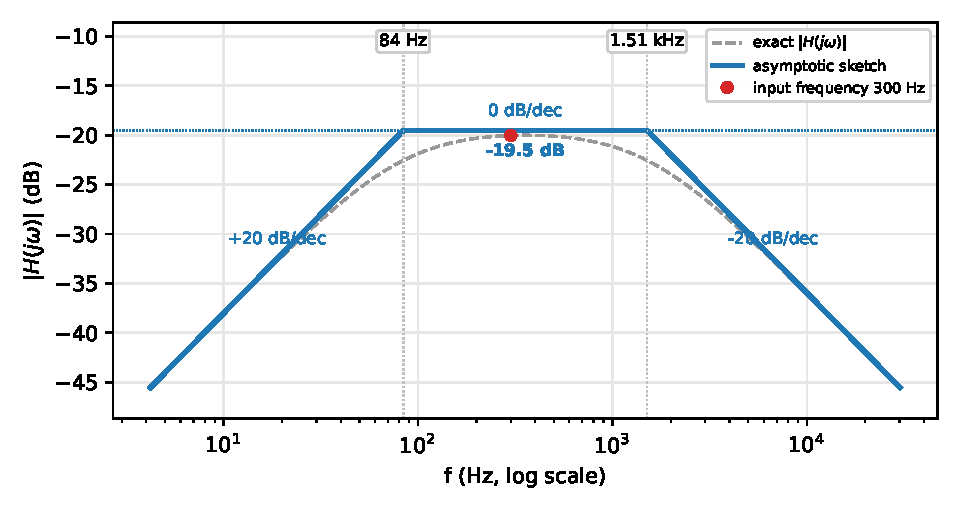
\includegraphics[width=0.78\linewidth,height=6.5cm,keepaspectratio]{p09_bode}\end{center}

{\small Blue: the straight-line sketch you are expected to draw. Dashed grey: the exact curve (about 3\,dB below the corner of an isolated pole). Red dot: the input frequency of Step 7.}
\solstep{7}{Steady-state output}The input is $V_i(t) = 1\sin\left(2\pi\cdot 300\,t\right)$, so $\omega_{in} = 2\pi\cdot 300 = 1880$\,rad/s. Put $s=j\omega_{in}$ in each factor (tool T5): magnitudes multiply, angles add.
{\small Rules: $\left|\frac{s}{s+p}\right| = \frac{\omega}{\sqrt{\omega^2+p^2}}$, $\angle = \frac{\pi}{2}-\tan^{-1}\frac{\omega}{p}$;\quad $\left|\frac{1}{1+s/p}\right| = \frac{1}{\sqrt{1+(\omega/p)^2}}$, $\angle = -\tan^{-1}\frac{\omega}{p}$;\quad $\left|1+\frac{s}{z}\right| = \sqrt{1+(\omega/z)^2}$, $\angle = \tan^{-1}\frac{\omega}{z}$;\quad a negative $K$ adds $-\pi$.}
\begin{center}\renewcommand{\arraystretch}{1.35}
\begin{tabular}{ccc}
\toprule
factor & magnitude & angle (rad) \\
\midrule
$-0.106$ & $0.1056$ & $-3.14$ \\
$\rule[-1.1em]{0pt}{2.8em}\dfrac{s}{s+2\pi\cdot 84}$ & $0.963$ & $0.273$ \\
$\rule[-1.7em]{0pt}{4em}\dfrac{1}{1+\dfrac{s}{2\pi\cdot 1.51\mathrm{k}}}$ & $0.9808$ & $-0.196$ \\
\textbf{total} & $\mathbf{0.09971}$ (product) & $\mathbf{-3.06}$ (sum) \\
\bottomrule
\end{tabular}\end{center}

\begin{align*}
|H(j\omega_{in})| &= 0.0997, \qquad \angle H(j\omega_{in}) = -3.06\ \mathrm{rad} \\
v_{o,ac}(t) &= 0.0997\times 1\,\sin\left(2\pi\cdot 300\,t - 3.06\right) = 0.0997\,\sin\left(2\pi\cdot 300\,t - 3.06\right)
\end{align*}

\[
\boxed{V_o(t) = 0.0997\,\sin\left(2\pi\cdot 300\,t - 3.06\right)\ \mathrm{V}}
\]

\begin{ansbox}
$H(s) = -0.106\,\dfrac{s}{s+2\pi\cdot 84}\,\dfrac{1}{1+\dfrac{s}{2\pi\cdot 1.51\mathrm{k}}}$\quad (corners: 84 Hz, 1.51 kHz)\\[4pt]
$V_o(t) = 0.0997\,\sin\left(2\pi\cdot 300\,t - 3.06\right)\ \mathrm{V}$
\end{ansbox}

\newpage
\subsection*{Solution 2B.10 \hfill Medium}
\begin{center}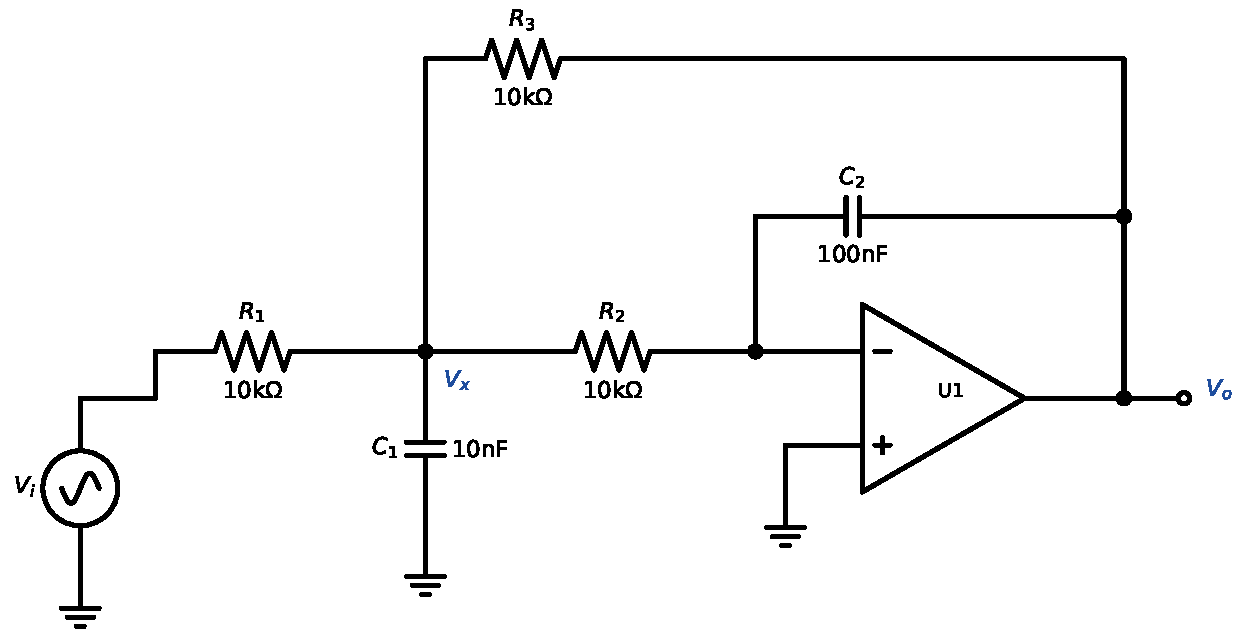
\includegraphics[width=\linewidth,height=5cm,keepaspectratio]{p10_circuit}\end{center}
\solstep{1}{Identify the sources}Independent sources: the AC input $V_i(t)$. No DC source: $V_{o,dc}=0$ and Step 2 is skipped.
\solstep{2}{DC circuit}No DC sources: $V_{o,dc}=0$.
\solstep{3}{Op-amp rules}Each op-amp has negative feedback (its output is connected back to its $-$ input), so with an ideal op-amp (tool T1): (a) no current flows into the $+$ or $-$ input; (b) $V_-=V_+$ (virtual short). The circuit is not a standard block, so it is solved by nodal analysis (tools T3, T4).
\solstep{4}{Transfer function by nodal analysis}\textbf{Block 1 (U1).} Multiple-feedback stage: node $V_x$ is fed back from the output through a second branch. This is not a standard block, so use nodal analysis. Virtual short (tool T1): U1: $V_- = V_+$, so $V_{-}$ is the same voltage as $0$ (virtual ground).
KCL (tool T3) at every node that is not an op-amp output or a source; no current flows into the op-amp inputs, so the op-amps do not appear in these sums:
\begin{align*}
&\text{(1) at }V_{-}\,(=0): && \frac{0 - V_{x}}{R_{2}} + sC_{2}\left(0 - V_{o}\right) = 0 \\
&\text{(2) at }V_{x}: && \frac{V_{x} - V_{i}}{R_{1}} + \frac{V_{x}}{R_{2}} + \frac{V_{x} - V_{o}}{R_{3}} + sC_{1}V_{x} = 0
\end{align*}

Solve them one at a time (tool T4): take the equation with the fewest unknowns, solve it for one node voltage and substitute that into the remaining equations. With the component values:
\begin{align*}
\text{from (1):}\quad V_{x} &= -0.001\,s\,V_{o}
\end{align*}

Substituting everything into (2) leaves only $V_{o}$ and $V_i$.\[
\frac{V_{o}}{V_i} = \dfrac{-10^{7}}{s^{2} + 30000\,s + 10^{7}}
\]

So:\[
H(s) = \dfrac{-10^{7}}{s^{2} + 30000\,s + 10^{7}}
\]

\solstep{5}{Standard (Bode-ready) form}Find the roots. Every root $s=-p$ of the denominator is a \emph{pole}, every root $s=-z$ of the numerator is a \emph{zero}; $|p|$ and $|z|$ are the corner frequencies (rad/s).
\begin{itemize}[leftmargin=*,itemsep=2pt]
\item Denominator: $s^{2} + 30000\,s + 10^{7}$; quadratic formula:\[
s = \frac{-30000 \pm \sqrt{(30000)^2 - 4(10^{7})}}{2} = \frac{-30000 \pm 29300}{2} \Rightarrow s = -337,\ -29700
\]

\end{itemize}

Factored form (leading coefficient in front):
\[
H(s) = -10^{7}\,\dfrac{1}{(s+337)(s+29700)}
\]

Bode-ready form: rewrite every $(s+p) = p\left(1+\frac{s}{p}\right)$ and $(s+z) = z\left(1+\frac{s}{z}\right)$, and collect all constants into $K$. Then every factor except $K$ is $\approx 1$ inside the pass-band:
\[
H(s) = -1\,\dfrac{1}{1+\dfrac{s}{2\pi\cdot 53.7}}\,\dfrac{1}{1+\dfrac{s}{2\pi\cdot 4.72\mathrm{k}}},\qquad K = -1
\]

\begin{center}\renewcommand{\arraystretch}{1.35}
\begin{tabular}{cccc}
\toprule
type & $\omega_c$ (rad/s) & $f_c=\omega_c/2\pi$ & slope change \\
\midrule
pole & $337$ & 53.7 Hz & $-20$ dB/dec \\
pole & $29700$ & 4.72 kHz & $-20$ dB/dec \\
\bottomrule
\end{tabular}\end{center}

\solstep{6}{Magnitude Bode plot}Below every corner, all factors are $\approx$ constant: $|H| \approx 1$ $= -0.000000000000000964$\,dB (flat, 0 dB/dec). Then, moving right, each pole bends the line down by 20\,dB/dec and each zero bends it up by 20\,dB/dec (tool T6):
\begin{center}\renewcommand{\arraystretch}{1.35}
\begin{tabular}{lcl}
\toprule
frequency range & slope & asymptote level \\
\midrule
$f<$ 53.7 Hz & $0$ dB/dec (flat) & 0 dB at end \\
53.7 Hz -- 4.72 kHz & $-20$ dB/dec & 0 dB at start, -38.9 dB at end \\
$f>$ 4.72 kHz & $-40$ dB/dec & -38.9 dB at start \\
\bottomrule
\end{tabular}\end{center}

The flat (pass-band) level is $20\log_{10}|K| = 20\log_{10}1 = -0.000000000000000964$\,dB.
\begin{center}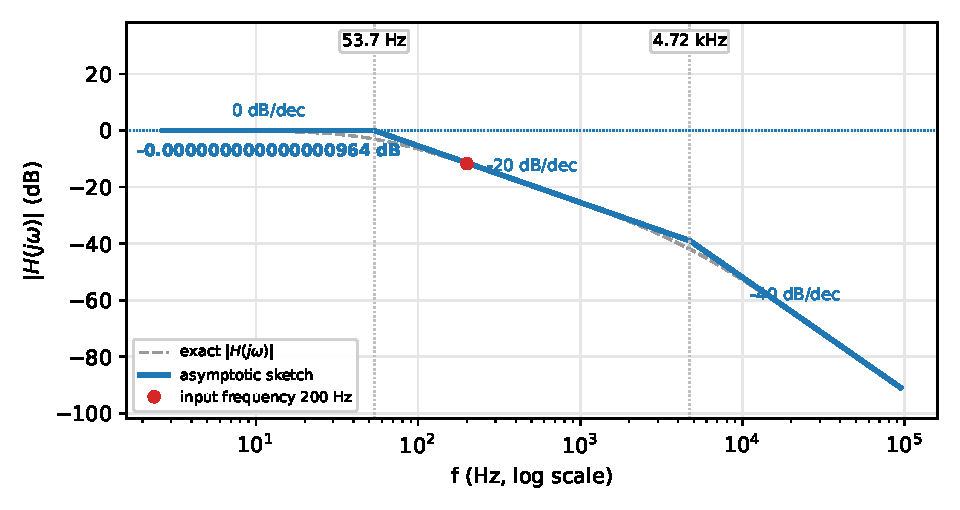
\includegraphics[width=0.78\linewidth,height=6.5cm,keepaspectratio]{p10_bode}\end{center}

{\small Blue: the straight-line sketch you are expected to draw. Dashed grey: the exact curve (about 3\,dB below the corner of an isolated pole). Red dot: the input frequency of Step 7.}
\solstep{7}{Steady-state output}The input is $V_i(t) = 0.5\sin\left(2\pi\cdot 200\,t\right)$, so $\omega_{in} = 2\pi\cdot 200 = 1260$\,rad/s. Put $s=j\omega_{in}$ in each factor (tool T5): magnitudes multiply, angles add.
{\small Rules: $\left|\frac{s}{s+p}\right| = \frac{\omega}{\sqrt{\omega^2+p^2}}$, $\angle = \frac{\pi}{2}-\tan^{-1}\frac{\omega}{p}$;\quad $\left|\frac{1}{1+s/p}\right| = \frac{1}{\sqrt{1+(\omega/p)^2}}$, $\angle = -\tan^{-1}\frac{\omega}{p}$;\quad $\left|1+\frac{s}{z}\right| = \sqrt{1+(\omega/z)^2}$, $\angle = \tan^{-1}\frac{\omega}{z}$;\quad a negative $K$ adds $-\pi$.}
\begin{center}\renewcommand{\arraystretch}{1.35}
\begin{tabular}{ccc}
\toprule
factor & magnitude & angle (rad) \\
\midrule
$-1$ & $1$ & $-3.14$ \\
$\rule[-1.7em]{0pt}{4em}\dfrac{1}{1+\dfrac{s}{2\pi\cdot 53.7}}$ & $0.2591$ & $-1.31$ \\
$\rule[-1.7em]{0pt}{4em}\dfrac{1}{1+\dfrac{s}{2\pi\cdot 4.72\mathrm{k}}}$ & $0.9991$ & $-0.0423$ \\
\textbf{total} & $\mathbf{0.2589}$ (product) & $\mathbf{-4.49}$ (sum) \\
\bottomrule
\end{tabular}\end{center}

\begin{align*}
|H(j\omega_{in})| &= 0.259, \qquad \angle H(j\omega_{in}) = -4.49\ \mathrm{rad} \\
v_{o,ac}(t) &= 0.259\times 0.5\,\sin\left(2\pi\cdot 200\,t - 4.49\right) = 0.129\,\sin\left(2\pi\cdot 200\,t - 4.49\right)
\end{align*}

\[
\boxed{V_o(t) = 0.129\,\sin\left(2\pi\cdot 200\,t - 4.49\right)\ \mathrm{V}}
\]

\begin{ansbox}
$H(s) = -1\,\dfrac{1}{1+\dfrac{s}{2\pi\cdot 53.7}}\,\dfrac{1}{1+\dfrac{s}{2\pi\cdot 4.72\mathrm{k}}}$\quad (corners: 53.7 Hz, 4.72 kHz)\\[4pt]
$V_o(t) = 0.129\,\sin\left(2\pi\cdot 200\,t - 4.49\right)\ \mathrm{V}$
\end{ansbox}

\newpage
\subsection*{Solution 2B.11 \hfill Medium}
\begin{center}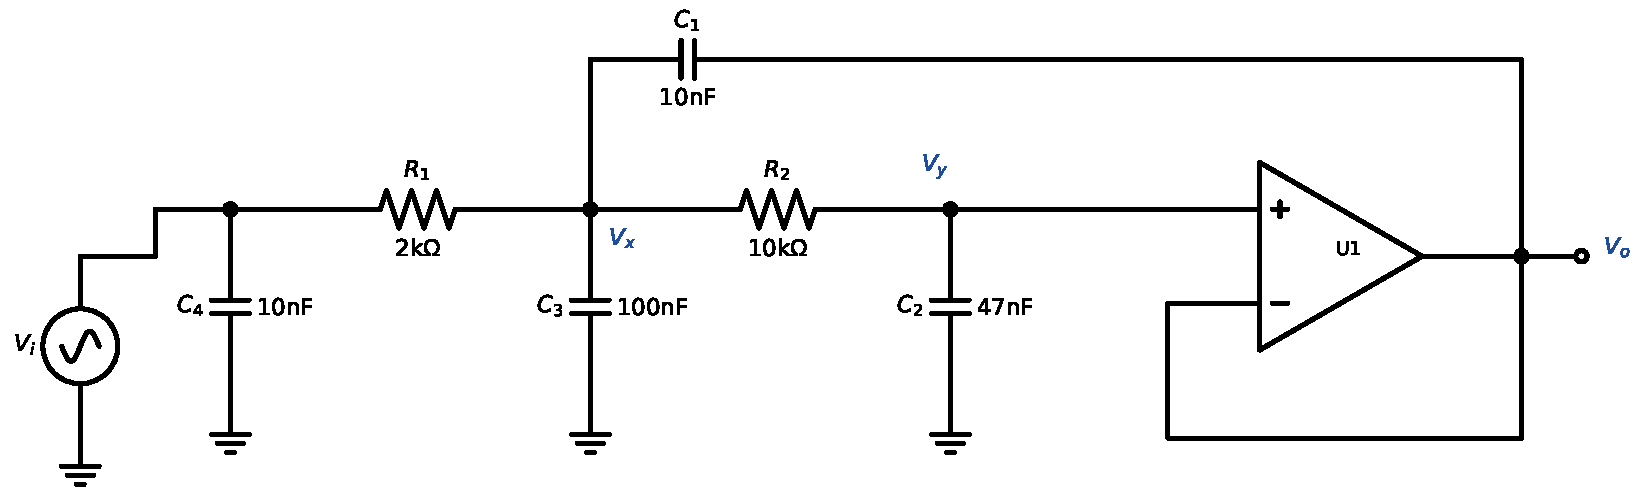
\includegraphics[width=\linewidth,height=5cm,keepaspectratio]{p11_circuit}\end{center}
\solstep{1}{Identify the sources}Independent sources: the AC input $V_i(t)$. No DC source: $V_{o,dc}=0$ and Step 2 is skipped.
\solstep{2}{DC circuit}No DC sources: $V_{o,dc}=0$.
\solstep{3}{Op-amp rules}Each op-amp has negative feedback (its output is connected back to its $-$ input), so with an ideal op-amp (tool T1): (a) no current flows into the $+$ or $-$ input; (b) $V_-=V_+$ (virtual short). The circuit is not a standard block, so it is solved by nodal analysis (tools T3, T4).
\solstep{4}{Transfer function by nodal analysis}\textbf{Block 1 (U1).} Sallen-Key stage: the network feeds back from the output to node $V_x$. This is not a standard block, so use nodal analysis. Virtual short (tool T1): U1: $V_- = V_+$, so $V_{o}$ is the same voltage as $V_{y}$.
KCL (tool T3) at every node that is not an op-amp output or a source; no current flows into the op-amp inputs, so the op-amps do not appear in these sums:
\begin{align*}
&\text{(1) at }V_{x}: && \frac{V_{x} - V_{i}}{R_{1}} + \frac{V_{x} - V_{y}}{R_{2}} + sC_{1}\left(V_{x} - V_{y}\right) + sC_{3}V_{x} = 0 \\
&\text{(2) at }V_{y}: && \frac{V_{y} - V_{x}}{R_{2}} + sC_{2}V_{y} = 0
\end{align*}

Solve them one at a time (tool T4): take the equation with the fewest unknowns, solve it for one node voltage and substitute that into the remaining equations. With the component values:
\begin{align*}
\text{from (1):}\quad V_{x} &= \left(\dfrac{0.0909\,s + 909}{s + 5450}\right)V_{y} + \left(\dfrac{4550}{s + 5450}\right)V_i
\end{align*}

Substituting everything into (2) leaves only $V_{y}$ and $V_i$. Since $V_{o} = V_{y}$ (virtual short),\[
\frac{V_{o}}{V_i} = \frac{V_{y}}{V_i} = \dfrac{9.67\times 10^{6}}{s^{2} + 7390\,s + 9.67\times 10^{6}}
\]

So:\[
H(s) = \dfrac{9.67\times 10^{6}}{s^{2} + 7390\,s + 9.67\times 10^{6}}
\]

\solstep{5}{Standard (Bode-ready) form}Find the roots. Every root $s=-p$ of the denominator is a \emph{pole}, every root $s=-z$ of the numerator is a \emph{zero}; $|p|$ and $|z|$ are the corner frequencies (rad/s).
\begin{itemize}[leftmargin=*,itemsep=2pt]
\item Denominator: $s^{2} + 7390\,s + 9.67\times 10^{6}$; quadratic formula:\[
s = \frac{-7390 \pm \sqrt{(7390)^2 - 4(9.67\times 10^{6})}}{2} = \frac{-7390 \pm 3990}{2} \Rightarrow s = -1700,\ -5690
\]

\end{itemize}

Factored form (leading coefficient in front):
\[
H(s) = 9.67\times 10^{6}\,\dfrac{1}{(s+1700)(s+5690)}
\]

Bode-ready form: rewrite every $(s+p) = p\left(1+\frac{s}{p}\right)$ and $(s+z) = z\left(1+\frac{s}{z}\right)$, and collect all constants into $K$. Then every factor except $K$ is $\approx 1$ inside the pass-band:
\[
H(s) = 1\,\dfrac{1}{1+\dfrac{s}{2\pi\cdot 271}}\,\dfrac{1}{1+\dfrac{s}{2\pi\cdot 905}},\qquad K = 1
\]

\begin{center}\renewcommand{\arraystretch}{1.35}
\begin{tabular}{cccc}
\toprule
type & $\omega_c$ (rad/s) & $f_c=\omega_c/2\pi$ & slope change \\
\midrule
pole & $1700$ & 271 Hz & $-20$ dB/dec \\
pole & $5690$ & 905 Hz & $-20$ dB/dec \\
\bottomrule
\end{tabular}\end{center}

\solstep{6}{Magnitude Bode plot}Below every corner, all factors are $\approx$ constant: $|H| \approx 1$ $= 0$\,dB (flat, 0 dB/dec). Then, moving right, each pole bends the line down by 20\,dB/dec and each zero bends it up by 20\,dB/dec (tool T6):
\begin{center}\renewcommand{\arraystretch}{1.35}
\begin{tabular}{lcl}
\toprule
frequency range & slope & asymptote level \\
\midrule
$f<$ 271 Hz & $0$ dB/dec (flat) & 0 dB at end \\
271 Hz -- 905 Hz & $-20$ dB/dec & 0 dB at start, -10.5 dB at end \\
$f>$ 905 Hz & $-40$ dB/dec & -10.5 dB at start \\
\bottomrule
\end{tabular}\end{center}

The flat (pass-band) level is $20\log_{10}|K| = 20\log_{10}1 = 0$\,dB.
\begin{center}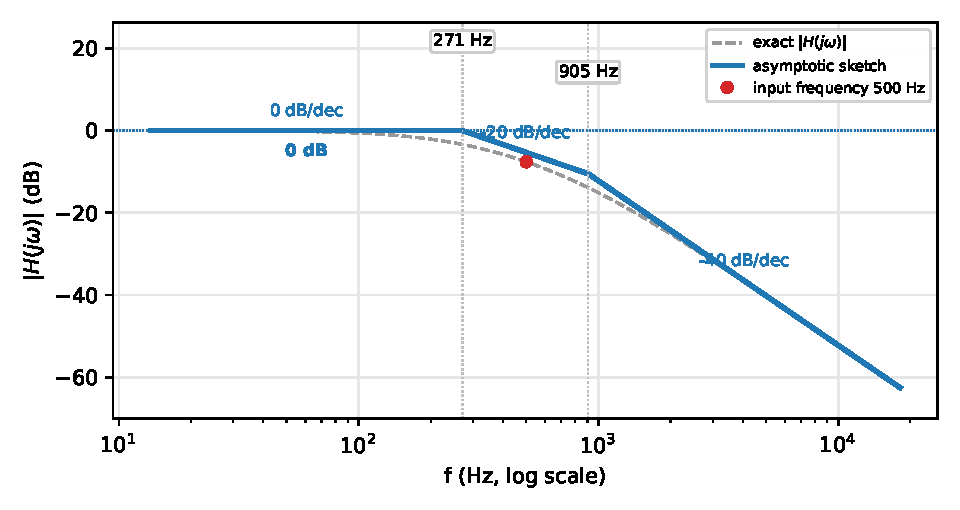
\includegraphics[width=0.78\linewidth,height=6.5cm,keepaspectratio]{p11_bode}\end{center}

{\small Blue: the straight-line sketch you are expected to draw. Dashed grey: the exact curve (about 3\,dB below the corner of an isolated pole). Red dot: the input frequency of Step 7.}
\solstep{7}{Steady-state output}The input is $V_i(t) = 0.5\sin\left(2\pi\cdot 500\,t+\frac{\pi}{4}\right)$, so $\omega_{in} = 2\pi\cdot 500 = 3140$\,rad/s. Put $s=j\omega_{in}$ in each factor (tool T5): magnitudes multiply, angles add.
{\small Rules: $\left|\frac{s}{s+p}\right| = \frac{\omega}{\sqrt{\omega^2+p^2}}$, $\angle = \frac{\pi}{2}-\tan^{-1}\frac{\omega}{p}$;\quad $\left|\frac{1}{1+s/p}\right| = \frac{1}{\sqrt{1+(\omega/p)^2}}$, $\angle = -\tan^{-1}\frac{\omega}{p}$;\quad $\left|1+\frac{s}{z}\right| = \sqrt{1+(\omega/z)^2}$, $\angle = \tan^{-1}\frac{\omega}{z}$;\quad a negative $K$ adds $-\pi$.}
\begin{center}\renewcommand{\arraystretch}{1.35}
\begin{tabular}{ccc}
\toprule
factor & magnitude & angle (rad) \\
\midrule
$1$ & $1$ & $0$ \\
$\rule[-1.7em]{0pt}{4em}\dfrac{1}{1+\dfrac{s}{2\pi\cdot 271}}$ & $0.4759$ & $-1.07$ \\
$\rule[-1.7em]{0pt}{4em}\dfrac{1}{1+\dfrac{s}{2\pi\cdot 905}}$ & $0.8754$ & $-0.505$ \\
\textbf{total} & $\mathbf{0.4166}$ (product) & $\mathbf{-1.58}$ (sum) \\
\bottomrule
\end{tabular}\end{center}

\begin{align*}
|H(j\omega_{in})| &= 0.417, \qquad \angle H(j\omega_{in}) = -1.58\ \mathrm{rad} \\
v_{o,ac}(t) &= 0.417\times 0.5\,\sin\left(2\pi\cdot 500\,t - 0.794\right) = 0.208\,\sin\left(2\pi\cdot 500\,t - 0.794\right)
\end{align*}

(phase: $\theta + \angle H = \frac{\pi}{4} + (-1.58) = -0.794$\,rad.)
\[
\boxed{V_o(t) = 0.208\,\sin\left(2\pi\cdot 500\,t - 0.794\right)\ \mathrm{V}}
\]

\begin{ansbox}
$H(s) = 1\,\dfrac{1}{1+\dfrac{s}{2\pi\cdot 271}}\,\dfrac{1}{1+\dfrac{s}{2\pi\cdot 905}}$\quad (corners: 271 Hz, 905 Hz)\\[4pt]
$V_o(t) = 0.208\,\sin\left(2\pi\cdot 500\,t - 0.794\right)\ \mathrm{V}$
\end{ansbox}

\newpage
\subsection*{Solution 2B.12 \hfill Medium}
\begin{center}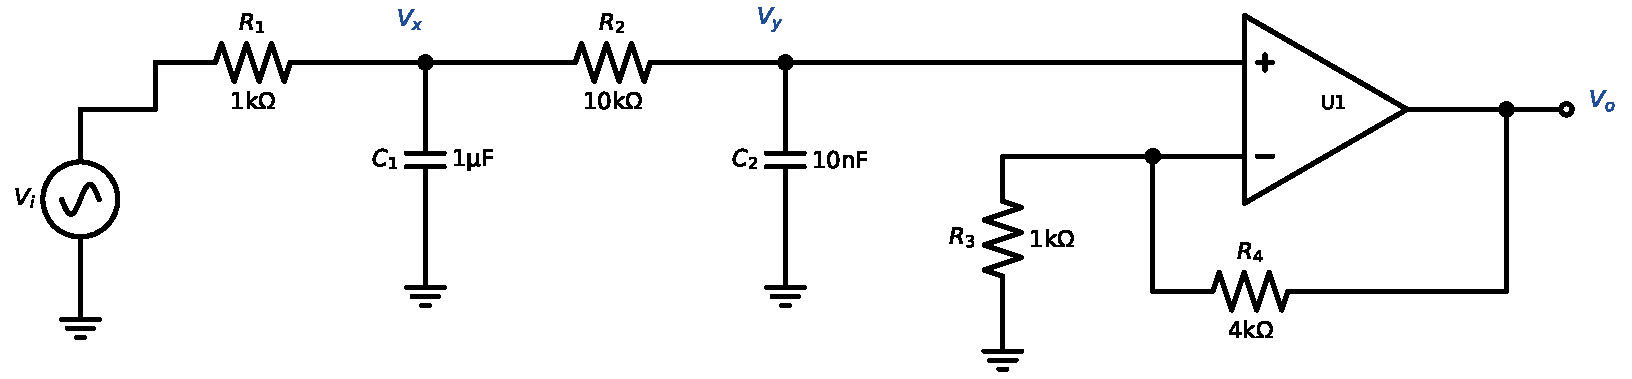
\includegraphics[width=\linewidth,height=5cm,keepaspectratio]{p12_circuit}\end{center}
\solstep{1}{Identify the sources}Independent sources: the AC input $V_i(t)$. No DC source: $V_{o,dc}=0$ and Step 2 is skipped.
\solstep{2}{DC circuit}No DC sources: $V_{o,dc}=0$.
\solstep{3}{Op-amp rules}Each op-amp has negative feedback (its output is connected back to its $-$ input), so with an ideal op-amp (tool T1): (a) no current flows into the $+$ or $-$ input; (b) $V_-=V_+$ (virtual short). The circuit is not a standard block, so it is solved by nodal analysis (tools T3, T4).
\solstep{4}{Transfer function by nodal analysis}\textbf{Block 1 (U1).} A two-section passive ladder drives the $+$ input. This is not a standard block, so use nodal analysis. Virtual short (tool T1): U1: $V_- = V_+$, so $V_{-}$ is the same voltage as $V_{y}$.
KCL (tool T3) at every node that is not an op-amp output or a source; no current flows into the op-amp inputs, so the op-amps do not appear in these sums:
\begin{align*}
&\text{(1) at }V_{-}\,(=V_{y}): && \frac{V_{y}}{R_{3}} + \frac{V_{y} - V_{o}}{R_{4}} = 0 \\
&\text{(2) at }V_{x}: && \frac{V_{x} - V_{i}}{R_{1}} + sC_{1}V_{x} + \frac{V_{x} - V_{y}}{R_{2}} = 0 \\
&\text{(3) at }V_{y}: && \frac{V_{y} - V_{x}}{R_{2}} + sC_{2}V_{y} = 0
\end{align*}

Solve them one at a time (tool T4): take the equation with the fewest unknowns, solve it for one node voltage and substitute that into the remaining equations. With the component values:
\begin{align*}
\text{from (1):}\quad V_{y} &= 0.2\,V_{o} \\
\text{from (2):}\quad V_{x} &= \left(\dfrac{20}{s + 1100}\right)V_{o} + \left(\dfrac{1000}{s + 1100}\right)V_i
\end{align*}

Substituting everything into (3) leaves only $V_{o}$ and $V_i$.\[
\frac{V_{o}}{V_i} = \dfrac{5\times 10^{7}}{s^{2} + 11100\,s + 10^{7}}
\]

So:\[
H(s) = \dfrac{5\times 10^{7}}{s^{2} + 11100\,s + 10^{7}}
\]

\solstep{5}{Standard (Bode-ready) form}Find the roots. Every root $s=-p$ of the denominator is a \emph{pole}, every root $s=-z$ of the numerator is a \emph{zero}; $|p|$ and $|z|$ are the corner frequencies (rad/s).
\begin{itemize}[leftmargin=*,itemsep=2pt]
\item Denominator: $s^{2} + 11100\,s + 10^{7}$; quadratic formula:\[
s = \frac{-11100 \pm \sqrt{(11100)^2 - 4(10^{7})}}{2} = \frac{-11100 \pm 9120}{2} \Rightarrow s = -989,\ -10100
\]

\end{itemize}

Factored form (leading coefficient in front):
\[
H(s) = 5\times 10^{7}\,\dfrac{1}{(s+989)(s+10100)}
\]

Bode-ready form: rewrite every $(s+p) = p\left(1+\frac{s}{p}\right)$ and $(s+z) = z\left(1+\frac{s}{z}\right)$, and collect all constants into $K$. Then every factor except $K$ is $\approx 1$ inside the pass-band:
\[
H(s) = 5\,\dfrac{1}{1+\dfrac{s}{2\pi\cdot 157}}\,\dfrac{1}{1+\dfrac{s}{2\pi\cdot 1.61\mathrm{k}}},\qquad K = 5
\]

\begin{center}\renewcommand{\arraystretch}{1.35}
\begin{tabular}{cccc}
\toprule
type & $\omega_c$ (rad/s) & $f_c=\omega_c/2\pi$ & slope change \\
\midrule
pole & $989$ & 157 Hz & $-20$ dB/dec \\
pole & $10100$ & 1.61 kHz & $-20$ dB/dec \\
\bottomrule
\end{tabular}\end{center}

\solstep{6}{Magnitude Bode plot}Below every corner, all factors are $\approx$ constant: $|H| \approx 5$ $= 14$\,dB (flat, 0 dB/dec). Then, moving right, each pole bends the line down by 20\,dB/dec and each zero bends it up by 20\,dB/dec (tool T6):
\begin{center}\renewcommand{\arraystretch}{1.35}
\begin{tabular}{lcl}
\toprule
frequency range & slope & asymptote level \\
\midrule
$f<$ 157 Hz & $0$ dB/dec (flat) & 14 dB at end \\
157 Hz -- 1.61 kHz & $-20$ dB/dec & 14 dB at start, -6.21 dB at end \\
$f>$ 1.61 kHz & $-40$ dB/dec & -6.21 dB at start \\
\bottomrule
\end{tabular}\end{center}

The flat (pass-band) level is $20\log_{10}|K| = 20\log_{10}5 = 14$\,dB.
\begin{center}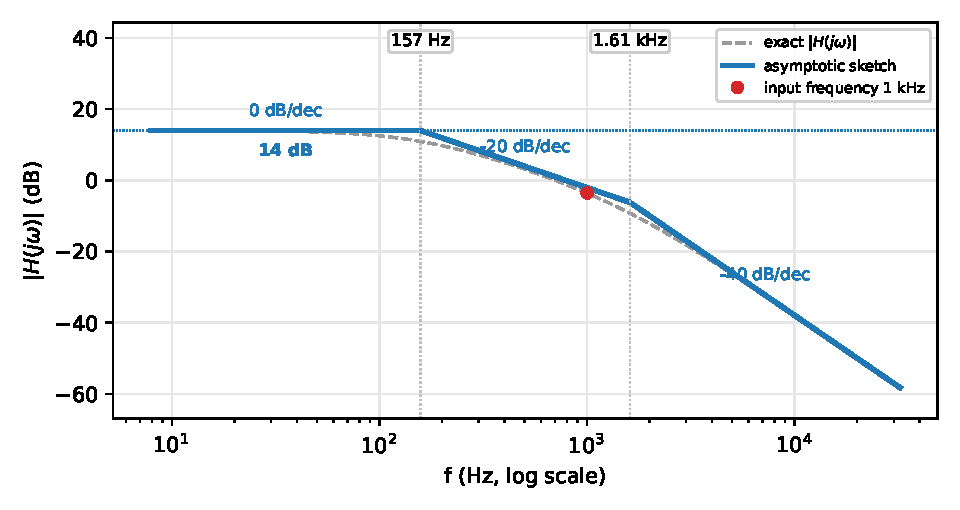
\includegraphics[width=0.78\linewidth,height=6.5cm,keepaspectratio]{p12_bode}\end{center}

{\small Blue: the straight-line sketch you are expected to draw. Dashed grey: the exact curve (about 3\,dB below the corner of an isolated pole). Red dot: the input frequency of Step 7.}
\solstep{7}{Steady-state output}The input is $V_i(t) = 0.1\sin\left(2\pi\cdot 1000\,t\right)$, so $\omega_{in} = 2\pi\cdot 1000 = 6280$\,rad/s. Put $s=j\omega_{in}$ in each factor (tool T5): magnitudes multiply, angles add.
{\small Rules: $\left|\frac{s}{s+p}\right| = \frac{\omega}{\sqrt{\omega^2+p^2}}$, $\angle = \frac{\pi}{2}-\tan^{-1}\frac{\omega}{p}$;\quad $\left|\frac{1}{1+s/p}\right| = \frac{1}{\sqrt{1+(\omega/p)^2}}$, $\angle = -\tan^{-1}\frac{\omega}{p}$;\quad $\left|1+\frac{s}{z}\right| = \sqrt{1+(\omega/z)^2}$, $\angle = \tan^{-1}\frac{\omega}{z}$;\quad a negative $K$ adds $-\pi$.}
\begin{center}\renewcommand{\arraystretch}{1.35}
\begin{tabular}{ccc}
\toprule
factor & magnitude & angle (rad) \\
\midrule
$5$ & $5$ & $0$ \\
$\rule[-1.7em]{0pt}{4em}\dfrac{1}{1+\dfrac{s}{2\pi\cdot 157}}$ & $0.1555$ & $-1.41$ \\
$\rule[-1.7em]{0pt}{4em}\dfrac{1}{1+\dfrac{s}{2\pi\cdot 1.61\mathrm{k}}}$ & $0.8494$ & $-0.556$ \\
\textbf{total} & $\mathbf{0.6604}$ (product) & $\mathbf{-1.97}$ (sum) \\
\bottomrule
\end{tabular}\end{center}

\begin{align*}
|H(j\omega_{in})| &= 0.66, \qquad \angle H(j\omega_{in}) = -1.97\ \mathrm{rad} \\
v_{o,ac}(t) &= 0.66\times 0.1\,\sin\left(2\pi\cdot 1000\,t - 1.97\right) = 0.066\,\sin\left(2\pi\cdot 1000\,t - 1.97\right)
\end{align*}

\[
\boxed{V_o(t) = 0.066\,\sin\left(2\pi\cdot 1000\,t - 1.97\right)\ \mathrm{V}}
\]

\begin{ansbox}
$H(s) = 5\,\dfrac{1}{1+\dfrac{s}{2\pi\cdot 157}}\,\dfrac{1}{1+\dfrac{s}{2\pi\cdot 1.61\mathrm{k}}}$\quad (corners: 157 Hz, 1.61 kHz)\\[4pt]
$V_o(t) = 0.066\,\sin\left(2\pi\cdot 1000\,t - 1.97\right)\ \mathrm{V}$
\end{ansbox}

\newpage
\subsection*{Solution 2B.13 \hfill Hard}
\begin{center}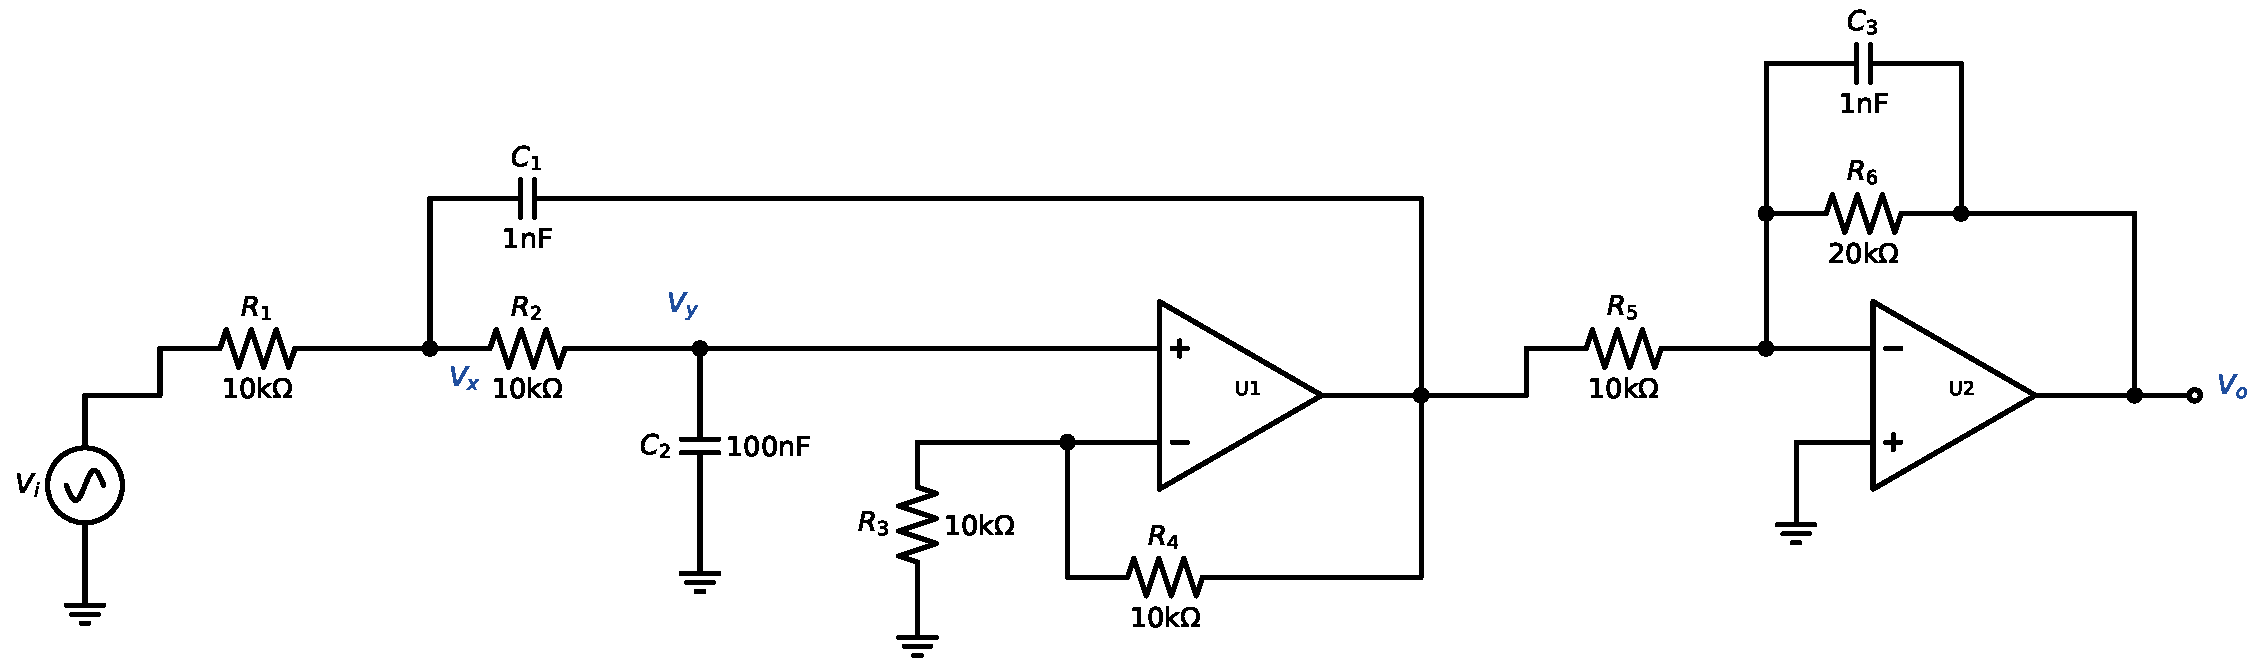
\includegraphics[width=\linewidth,height=5cm,keepaspectratio]{p13_circuit}\end{center}
\solstep{1}{Identify the sources}Independent sources: the AC input $V_i(t)$. No DC source: $V_{o,dc}=0$ and Step 2 is skipped.
\solstep{2}{DC circuit}No DC sources: $V_{o,dc}=0$.
\solstep{3}{Op-amp rules}Each op-amp has negative feedback (its output is connected back to its $-$ input), so with an ideal op-amp (tool T1): (a) no current flows into the $+$ or $-$ input; (b) $V_-=V_+$ (virtual short). Block 1 is not a standard block (nodal analysis, tools T3 and T4); the other blocks are standard (block formulas, tool T2). The blocks still multiply because every op-amp output is an ideal source.
\solstep{4}{Transfer function, block by block}Each op-amp output is an ideal voltage source, so a block's output does not change when the next block is connected: the blocks can be solved one at a time and multiplied.\[
H(s) = \frac{V_o}{V_i} = \frac{V_{o1}}{V_{i}}\cdot\frac{V_{o}}{V_{o1}}
\]

\textbf{Block 1 (U1).} Sallen-Key stage: the network feeds back from the output to node $V_x$. This is not a standard block, so use nodal analysis. Virtual short (tool T1): U1: $V_- = V_+$, so $V_{-}$ is the same voltage as $V_{y}$.
KCL (tool T3) at every node that is not an op-amp output or a source; no current flows into the op-amp inputs, so the op-amps do not appear in these sums:
\begin{align*}
&\text{(1) at }V_{-}\,(=V_{y}): && \frac{V_{y}}{R_{3}} + \frac{V_{y} - V_{o1}}{R_{4}} = 0 \\
&\text{(2) at }V_{x}: && \frac{V_{x} - V_{i}}{R_{1}} + \frac{V_{x} - V_{y}}{R_{2}} + sC_{1}\left(V_{x} - V_{o1}\right) = 0 \\
&\text{(3) at }V_{y}: && \frac{V_{y} - V_{x}}{R_{2}} + sC_{2}V_{y} = 0
\end{align*}

Solve them one at a time (tool T4): take the equation with the fewest unknowns, solve it for one node voltage and substitute that into the remaining equations. With the component values:
\begin{align*}
\text{from (1):}\quad V_{y} &= 0.5\,V_{o1} \\
\text{from (2):}\quad V_{x} &= \left(\dfrac{s + 50000}{s + 2\times 10^{5}}\right)V_{o1} + \left(\dfrac{10^{5}}{s + 2\times 10^{5}}\right)V_i
\end{align*}

Substituting everything into (3) leaves only $V_{o1}$ and $V_i$.\[
\frac{V_{o1}}{V_i} = \dfrac{2\times 10^{8}}{s^{2} + 1.99\times 10^{5}\,s + 10^{8}}
\]

\textbf{Block 2 (U2).} Inverting block: the $+$ input is grounded, so $V_- = V_+ = 0$ (virtual ground). The current $\frac{V_{o1} - 0}{R_{5}}$ through $R_{5}$ cannot enter the op-amp, so all of it flows through $Z_{f2}$: $V_{o} = 0 - Z_{f2}\cdot\frac{V_{o1}}{R_{5}}$.\begin{align*}
Z_{f2} &= R_{6} \parallel \frac{1}{sC_{3}} = \dfrac{10^{9}}{s + 50000}
\end{align*}
\[
\frac{V_{o}}{V_{o1}} = -\frac{Z_{f2}}{R_{5}} = \dfrac{-10^{5}}{s + 50000}
\]

Multiply the blocks and simplify:\[
H(s) = \dfrac{-2\times 10^{13}}{s^{3} + 2.49\times 10^{5}\,s^{2} + 10^{10}\,s + 5\times 10^{12}}
\]

\solstep{5}{Standard (Bode-ready) form}Find the roots. Every root $s=-p$ of the denominator is a \emph{pole}, every root $s=-z$ of the numerator is a \emph{zero}; $|p|$ and $|z|$ are the corner frequencies (rad/s).
\begin{itemize}[leftmargin=*,itemsep=2pt]
\item Denominator: $s^{3} + 2.49\times 10^{5}\,s^{2} + 10^{10}\,s + 5\times 10^{12}$; this is degree 3: use a calculator's polynomial solver (or \texttt{numpy.roots}) $\Rightarrow s = -504,\ -50000,\ -1.98\times 10^{5}$.
\end{itemize}

Factored form (leading coefficient in front):
\[
H(s) = -2\times 10^{13}\,\dfrac{1}{(s+504)(s+50000)(s+1.98\times 10^{5})}
\]

Bode-ready form: rewrite every $(s+p) = p\left(1+\frac{s}{p}\right)$ and $(s+z) = z\left(1+\frac{s}{z}\right)$, and collect all constants into $K$. Then every factor except $K$ is $\approx 1$ inside the pass-band:
\[
H(s) = -4\,\dfrac{1}{1+\dfrac{s}{2\pi\cdot 80.2}}\,\dfrac{1}{1+\dfrac{s}{2\pi\cdot 7.96\mathrm{k}}}\,\dfrac{1}{1+\dfrac{s}{2\pi\cdot 31.6\mathrm{k}}},\qquad K = -4
\]

\begin{center}\renewcommand{\arraystretch}{1.35}
\begin{tabular}{cccc}
\toprule
type & $\omega_c$ (rad/s) & $f_c=\omega_c/2\pi$ & slope change \\
\midrule
pole & $504$ & 80.2 Hz & $-20$ dB/dec \\
pole & $50000$ & 7.96 kHz & $-20$ dB/dec \\
pole & $1.98\times 10^{5}$ & 31.6 kHz & $-20$ dB/dec \\
\bottomrule
\end{tabular}\end{center}

\solstep{6}{Magnitude Bode plot}Below every corner, all factors are $\approx$ constant: $|H| \approx 4$ $= 12$\,dB (flat, 0 dB/dec). Then, moving right, each pole bends the line down by 20\,dB/dec and each zero bends it up by 20\,dB/dec (tool T6):
\begin{center}\renewcommand{\arraystretch}{1.35}
\begin{tabular}{lcl}
\toprule
frequency range & slope & asymptote level \\
\midrule
$f<$ 80.2 Hz & $0$ dB/dec (flat) & 12 dB at end \\
80.2 Hz -- 7.96 kHz & $-20$ dB/dec & 12 dB at start, -27.9 dB at end \\
7.96 kHz -- 31.6 kHz & $-40$ dB/dec & -27.9 dB at start, -51.8 dB at end \\
$f>$ 31.6 kHz & $-60$ dB/dec & -51.8 dB at start \\
\bottomrule
\end{tabular}\end{center}

The flat (pass-band) level is $20\log_{10}|K| = 20\log_{10}4 = 12$\,dB.
\begin{center}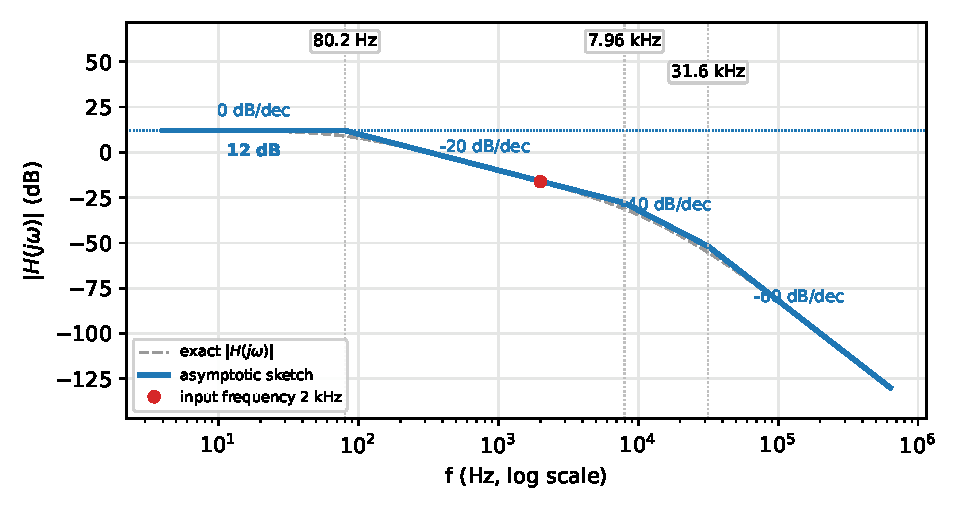
\includegraphics[width=0.78\linewidth,height=6.5cm,keepaspectratio]{p13_bode}\end{center}

{\small Blue: the straight-line sketch you are expected to draw. Dashed grey: the exact curve (about 3\,dB below the corner of an isolated pole). Red dot: the input frequency of Step 7.}
\solstep{7}{Steady-state output}The input is $V_i(t) = 0.1\sin\left(2\pi\cdot 2000\,t\right)$, so $\omega_{in} = 2\pi\cdot 2000 = 12600$\,rad/s. Put $s=j\omega_{in}$ in each factor (tool T5): magnitudes multiply, angles add.
{\small Rules: $\left|\frac{s}{s+p}\right| = \frac{\omega}{\sqrt{\omega^2+p^2}}$, $\angle = \frac{\pi}{2}-\tan^{-1}\frac{\omega}{p}$;\quad $\left|\frac{1}{1+s/p}\right| = \frac{1}{\sqrt{1+(\omega/p)^2}}$, $\angle = -\tan^{-1}\frac{\omega}{p}$;\quad $\left|1+\frac{s}{z}\right| = \sqrt{1+(\omega/z)^2}$, $\angle = \tan^{-1}\frac{\omega}{z}$;\quad a negative $K$ adds $-\pi$.}
\begin{center}\renewcommand{\arraystretch}{1.35}
\begin{tabular}{ccc}
\toprule
factor & magnitude & angle (rad) \\
\midrule
$-4$ & $4$ & $-3.14$ \\
$\rule[-1.7em]{0pt}{4em}\dfrac{1}{1+\dfrac{s}{2\pi\cdot 80.2}}$ & $0.04006$ & $-1.53$ \\
$\rule[-1.7em]{0pt}{4em}\dfrac{1}{1+\dfrac{s}{2\pi\cdot 7.96\mathrm{k}}}$ & $0.9698$ & $-0.246$ \\
$\rule[-1.7em]{0pt}{4em}\dfrac{1}{1+\dfrac{s}{2\pi\cdot 31.6\mathrm{k}}}$ & $0.998$ & $-0.0632$ \\
\textbf{total} & $\mathbf{0.1551}$ (product) & $\mathbf{-4.98}$ (sum) \\
\bottomrule
\end{tabular}\end{center}

\begin{align*}
|H(j\omega_{in})| &= 0.155, \qquad \angle H(j\omega_{in}) = -4.98\ \mathrm{rad} \\
v_{o,ac}(t) &= 0.155\times 0.1\,\sin\left(2\pi\cdot 2000\,t - 4.98\right) = 0.0155\,\sin\left(2\pi\cdot 2000\,t - 4.98\right)
\end{align*}

\[
\boxed{V_o(t) = 0.0155\,\sin\left(2\pi\cdot 2000\,t - 4.98\right)\ \mathrm{V}}
\]

\begin{ansbox}
$H(s) = -4\,\dfrac{1}{1+\dfrac{s}{2\pi\cdot 80.2}}\,\dfrac{1}{1+\dfrac{s}{2\pi\cdot 7.96\mathrm{k}}}\,\dfrac{1}{1+\dfrac{s}{2\pi\cdot 31.6\mathrm{k}}}$\quad (corners: 80.2 Hz, 7.96 kHz, 31.6 kHz)\\[4pt]
$V_o(t) = 0.0155\,\sin\left(2\pi\cdot 2000\,t - 4.98\right)\ \mathrm{V}$
\end{ansbox}

\newpage
\subsection*{Solution 2B.14 \hfill Hard}
\begin{center}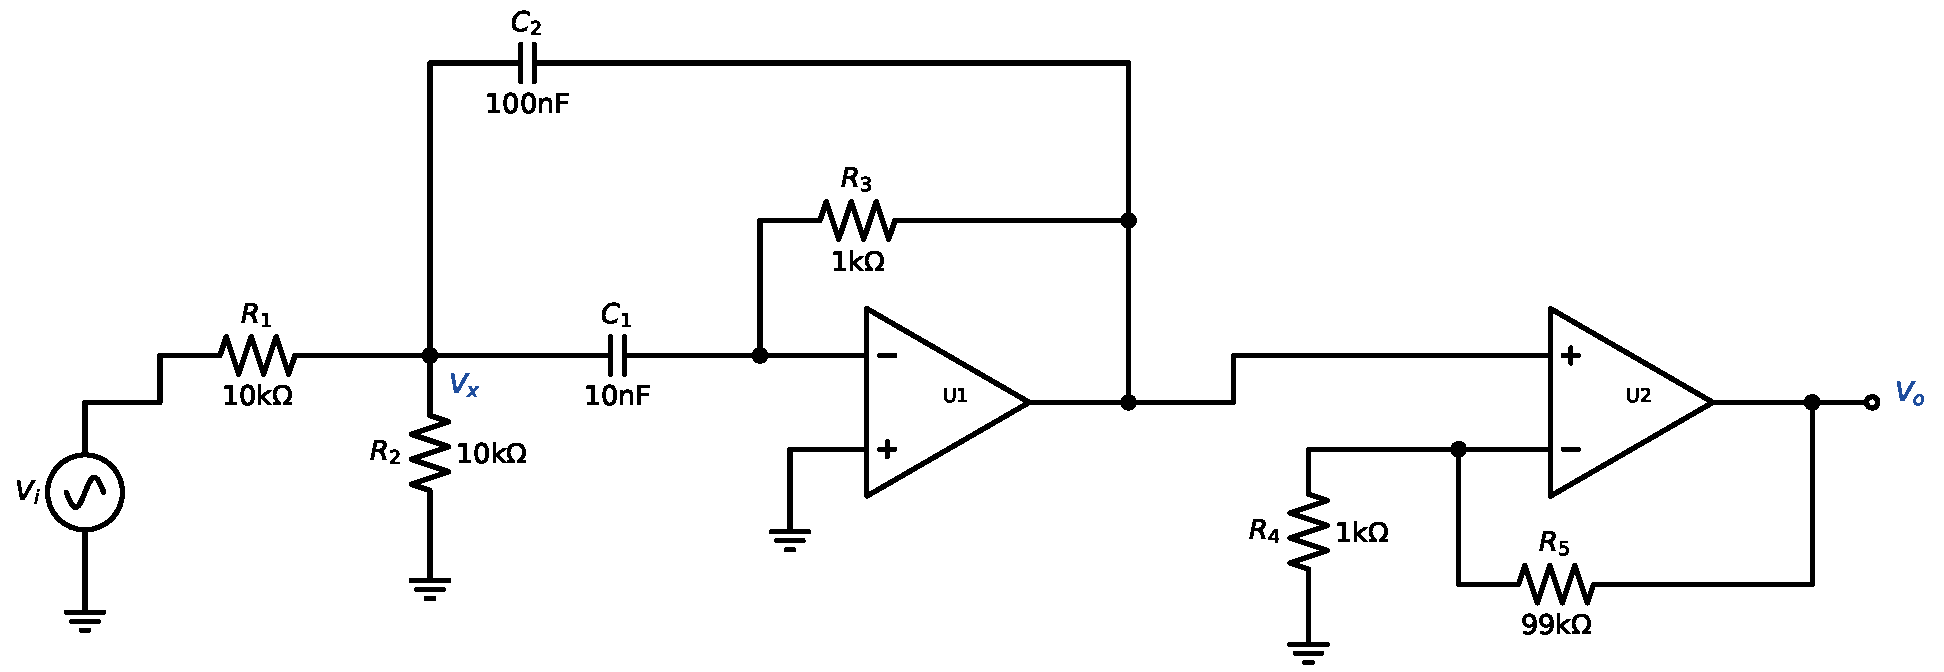
\includegraphics[width=\linewidth,height=5cm,keepaspectratio]{p14_circuit}\end{center}
\solstep{1}{Identify the sources}Independent sources: the AC input $V_i(t)$. No DC source: $V_{o,dc}=0$ and Step 2 is skipped.
\solstep{2}{DC circuit}No DC sources: $V_{o,dc}=0$.
\solstep{3}{Op-amp rules}Each op-amp has negative feedback (its output is connected back to its $-$ input), so with an ideal op-amp (tool T1): (a) no current flows into the $+$ or $-$ input; (b) $V_-=V_+$ (virtual short). Block 1 is not a standard block (nodal analysis, tools T3 and T4); the other blocks are standard (block formulas, tool T2). The blocks still multiply because every op-amp output is an ideal source.
\solstep{4}{Transfer function, block by block}Each op-amp output is an ideal voltage source, so a block's output does not change when the next block is connected: the blocks can be solved one at a time and multiplied.\[
H(s) = \frac{V_o}{V_i} = \frac{V_{o1}}{V_{i}}\cdot\frac{V_{o}}{V_{o1}}
\]

\textbf{Block 1 (U1).} Multiple-feedback stage: node $V_x$ is fed back from the output through a second branch. This is not a standard block, so use nodal analysis. Virtual short (tool T1): U1: $V_- = V_+$, so $V_{-}$ is the same voltage as $0$ (virtual ground).
KCL (tool T3) at every node that is not an op-amp output or a source; no current flows into the op-amp inputs, so the op-amps do not appear in these sums:
\begin{align*}
&\text{(1) at }V_{-}\,(=0): && sC_{1}\left(0 - V_{x}\right) + \frac{0 - V_{o1}}{R_{3}} = 0 \\
&\text{(2) at }V_{x}: && \frac{V_{x} - V_{i}}{R_{1}} + sC_{1}V_{x} + sC_{2}\left(V_{x} - V_{o1}\right) + \frac{V_{x}}{R_{2}} = 0
\end{align*}

Solve them one at a time (tool T4): take the equation with the fewest unknowns, solve it for one node voltage and substitute that into the remaining equations. With the component values:
\begin{align*}
\text{from (1):}\quad V_{x} &= \left(\dfrac{-10^{5}}{s}\right)V_{o1}
\end{align*}

Substituting everything into (2) leaves only $V_{o1}$ and $V_i$.\[
\frac{V_{o1}}{V_i} = \dfrac{-1000\,s}{s^{2} + 1.1\times 10^{5}\,s + 2\times 10^{8}}
\]

\textbf{Block 2 (U2).} Non-inverting block: The $+$ input is the block input: $V_+ = V_{o1}$. The op-amp forces $V_-=V_+$, and $R_{4}$, $R_{5}$ divide the output: $V_- = \frac{R_{4}}{R_{4} + R_{5}}V_{o}$, hence $V_{o} = \left(1+\frac{R_{5}}{R_{4}}\right)V_+$.\[
\frac{V_{o}}{V_{o1}} = \left(1+\frac{R_{5}}{R_{4}}\right) = 100
\]

Multiply the blocks and simplify:\[
H(s) = \dfrac{-10^{5}\,s}{s^{2} + 1.1\times 10^{5}\,s + 2\times 10^{8}}
\]

\solstep{5}{Standard (Bode-ready) form}Find the roots. Every root $s=-p$ of the denominator is a \emph{pole}, every root $s=-z$ of the numerator is a \emph{zero}; $|p|$ and $|z|$ are the corner frequencies (rad/s).
\begin{itemize}[leftmargin=*,itemsep=2pt]
\item Numerator: it has the factor $s$ $\Rightarrow$ 1 zero at $s=0$.
\item Denominator: $s^{2} + 1.1\times 10^{5}\,s + 2\times 10^{8}$; quadratic formula:\[
s = \frac{-1.1\times 10^{5} \pm \sqrt{(1.1\times 10^{5})^2 - 4(2\times 10^{8})}}{2} = \frac{-1.1\times 10^{5} \pm 1.06\times 10^{5}}{2} \Rightarrow s = -1850,\ -1.08\times 10^{5}
\]

\end{itemize}

Factored form (leading coefficient in front):
\[
H(s) = -10^{5}\,\dfrac{s}{(s+1850)(s+1.08\times 10^{5})}
\]

Bode-ready form: rewrite every $(s+p) = p\left(1+\frac{s}{p}\right)$ and $(s+z) = z\left(1+\frac{s}{z}\right)$, and collect all constants into $K$. Each $s$ in the numerator is paired with one of the \emph{lowest} poles as $\frac{s}{s+p}$ (that factor is $\approx 1$ above $p$). Then every factor except $K$ is $\approx 1$ inside the pass-band:
\[
H(s) = -0.925\,\dfrac{s}{s+2\pi\cdot 294}\,\dfrac{1}{1+\dfrac{s}{2\pi\cdot 17.2\mathrm{k}}},\qquad K = -0.925
\]

\begin{center}\renewcommand{\arraystretch}{1.35}
\begin{tabular}{cccc}
\toprule
type & $\omega_c$ (rad/s) & $f_c=\omega_c/2\pi$ & slope change \\
\midrule
pole & $1850$ & 294 Hz & $-20$ dB/dec \\
pole & $1.08\times 10^{5}$ & 17.2 kHz & $-20$ dB/dec \\
\bottomrule
\end{tabular}\end{center}

\solstep{6}{Magnitude Bode plot}Below every corner $|H(s)|\approx 5\times 10^{-4}\,s$, so the plot starts with a slope of $+20$\,dB/dec. Then, moving right, each pole bends the line down by 20\,dB/dec and each zero bends it up by 20\,dB/dec (tool T6):
\begin{center}\renewcommand{\arraystretch}{1.35}
\begin{tabular}{lcl}
\toprule
frequency range & slope & asymptote level \\
\midrule
$f<$ 294 Hz & $+20$ dB/dec & -0.681 dB at end \\
294 Hz -- 17.2 kHz & $0$ dB/dec (flat) & -0.681 dB at start, -0.681 dB at end \\
$f>$ 17.2 kHz & $-20$ dB/dec & -0.681 dB at start \\
\bottomrule
\end{tabular}\end{center}

The flat (pass-band) level is $20\log_{10}|K| = 20\log_{10}0.925 = -0.681$\,dB.
\begin{center}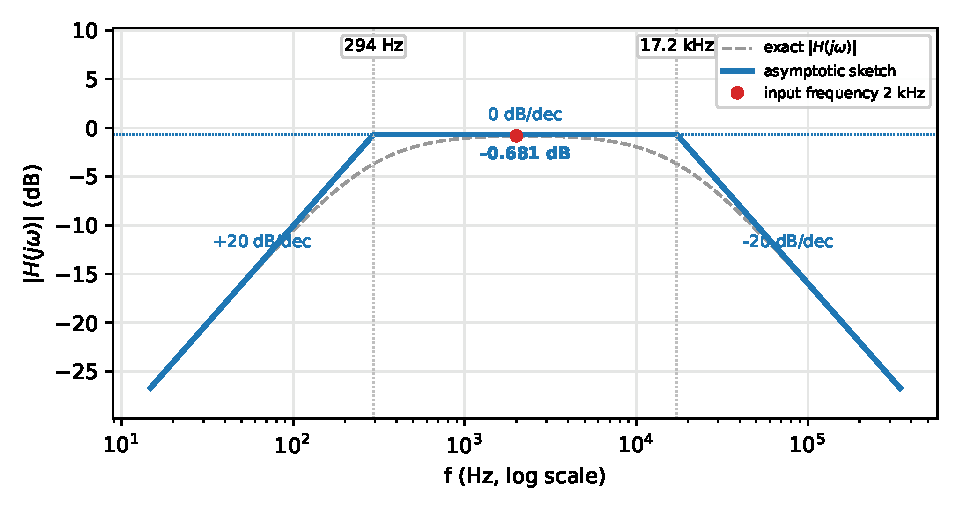
\includegraphics[width=0.78\linewidth,height=6.5cm,keepaspectratio]{p14_bode}\end{center}

{\small Blue: the straight-line sketch you are expected to draw. Dashed grey: the exact curve (about 3\,dB below the corner of an isolated pole). Red dot: the input frequency of Step 7.}
\solstep{7}{Steady-state output}The input is $V_i(t) = 0.05\sin\left(2\pi\cdot 2000\,t\right)$, so $\omega_{in} = 2\pi\cdot 2000 = 12600$\,rad/s. Put $s=j\omega_{in}$ in each factor (tool T5): magnitudes multiply, angles add.
{\small Rules: $\left|\frac{s}{s+p}\right| = \frac{\omega}{\sqrt{\omega^2+p^2}}$, $\angle = \frac{\pi}{2}-\tan^{-1}\frac{\omega}{p}$;\quad $\left|\frac{1}{1+s/p}\right| = \frac{1}{\sqrt{1+(\omega/p)^2}}$, $\angle = -\tan^{-1}\frac{\omega}{p}$;\quad $\left|1+\frac{s}{z}\right| = \sqrt{1+(\omega/z)^2}$, $\angle = \tan^{-1}\frac{\omega}{z}$;\quad a negative $K$ adds $-\pi$.}
\begin{center}\renewcommand{\arraystretch}{1.35}
\begin{tabular}{ccc}
\toprule
factor & magnitude & angle (rad) \\
\midrule
$-0.925$ & $0.9246$ & $-3.14$ \\
$\rule[-1.1em]{0pt}{2.8em}\dfrac{s}{s+2\pi\cdot 294}$ & $0.9893$ & $0.146$ \\
$\rule[-1.7em]{0pt}{4em}\dfrac{1}{1+\dfrac{s}{2\pi\cdot 17.2\mathrm{k}}}$ & $0.9933$ & $-0.116$ \\
\textbf{total} & $\mathbf{0.9087}$ (product) & $\mathbf{-3.11}$ (sum) \\
\bottomrule
\end{tabular}\end{center}

\begin{align*}
|H(j\omega_{in})| &= 0.909, \qquad \angle H(j\omega_{in}) = -3.11\ \mathrm{rad} \\
v_{o,ac}(t) &= 0.909\times 0.05\,\sin\left(2\pi\cdot 2000\,t - 3.11\right) = 0.0454\,\sin\left(2\pi\cdot 2000\,t - 3.11\right)
\end{align*}

\[
\boxed{V_o(t) = 0.0454\,\sin\left(2\pi\cdot 2000\,t - 3.11\right)\ \mathrm{V}}
\]

\begin{ansbox}
$H(s) = -0.925\,\dfrac{s}{s+2\pi\cdot 294}\,\dfrac{1}{1+\dfrac{s}{2\pi\cdot 17.2\mathrm{k}}}$\quad (corners: 294 Hz, 17.2 kHz)\\[4pt]
$V_o(t) = 0.0454\,\sin\left(2\pi\cdot 2000\,t - 3.11\right)\ \mathrm{V}$
\end{ansbox}

\newpage
\subsection*{Solution 2B.15 \hfill Hard}
\begin{center}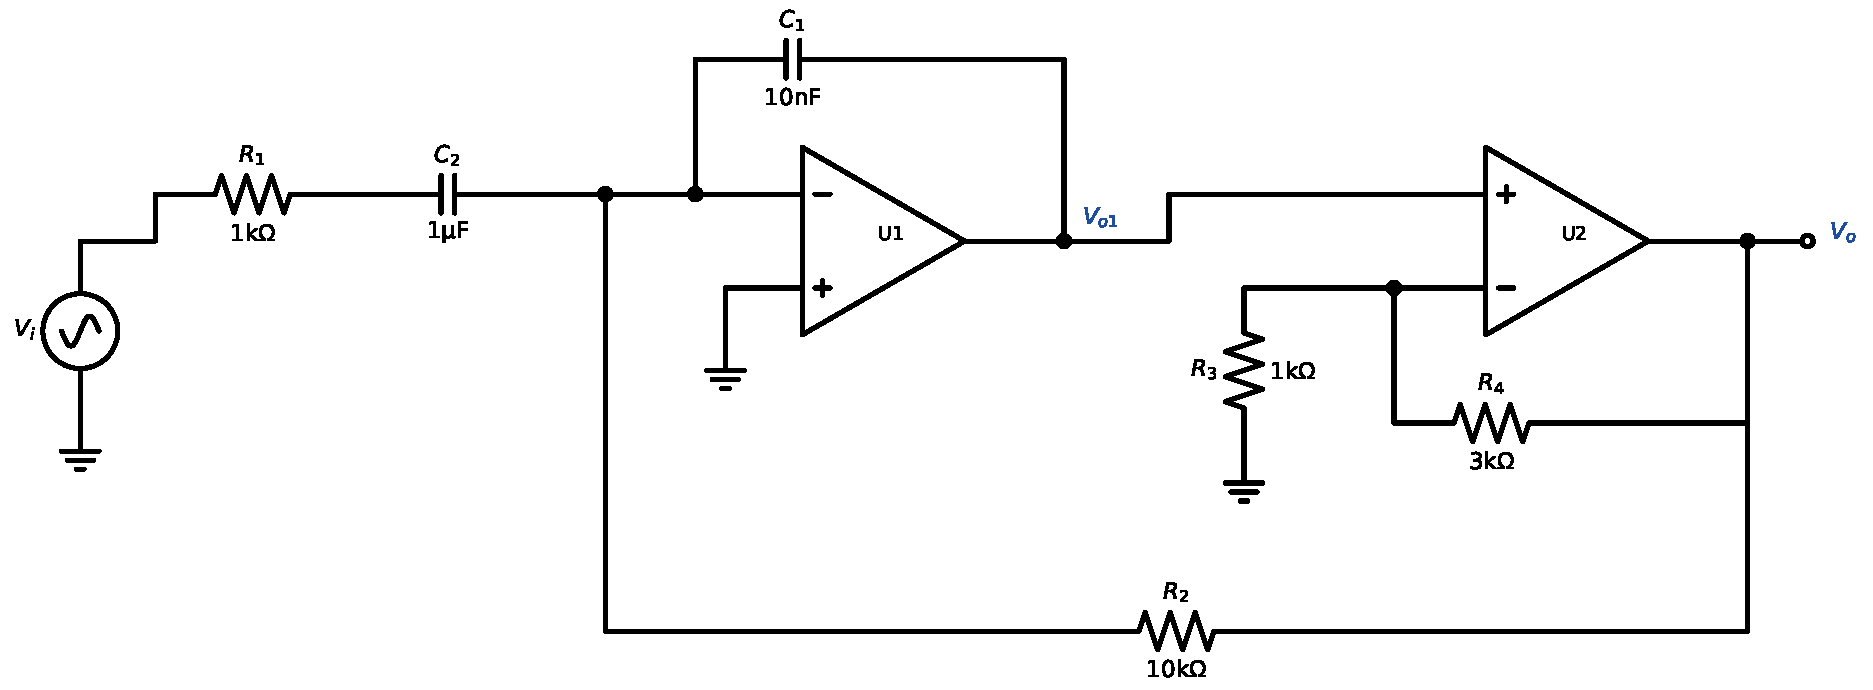
\includegraphics[width=\linewidth,height=5cm,keepaspectratio]{p15_circuit}\end{center}
\solstep{1}{Identify the sources}Independent sources: the AC input $V_i(t)$. No DC source: $V_{o,dc}=0$ and Step 2 is skipped.
\solstep{2}{DC circuit}No DC sources: $V_{o,dc}=0$.
\solstep{3}{Op-amp rules}Each op-amp has negative feedback (its output is connected back to its $-$ input), so with an ideal op-amp (tool T1): (a) no current flows into the $+$ or $-$ input; (b) $V_-=V_+$ (virtual short). The circuit is not a standard block, so it is solved by nodal analysis (tools T3, T4).
\solstep{4}{Transfer function by nodal analysis}\textbf{Block 1 (U1).} Two op-amps in a loop: $U_2$ amplifies $V_{o1}$ and feeds it back into the summing node of $U_1$, so the stages cannot simply be multiplied. This is not a standard block, so use nodal analysis. Short names for the composite branches:\begin{align*}
Z_{a} &= R_{1} + \frac{1}{sC_{2}} = \dfrac{1000\,s + 10^{6}}{s}
\end{align*}
Virtual short (tool T1): U1: $V_- = V_+$, so $V_{-}$ is the same voltage as $0$ (virtual ground). U2: $V_- = V_+$, so $V_{n}$ is the same voltage as $V_{o1}$.
KCL (tool T3) at every node that is not an op-amp output or a source; no current flows into the op-amp inputs, so the op-amps do not appear in these sums:
\begin{align*}
&\text{(1) at }V_{-}\,(=0): && \frac{0 - V_{i}}{Z_{a}} + sC_{1}\left(0 - V_{o1}\right) + \frac{0 - V_{o}}{R_{2}} = 0 \\
&\text{(2) at }V_{n}\,(=V_{o1}): && \frac{V_{o1}}{R_{3}} + \frac{V_{o1} - V_{o}}{R_{4}} = 0
\end{align*}

Solve them one at a time (tool T4): take the equation with the fewest unknowns, solve it for one node voltage and substitute that into the remaining equations. With the component values:
\begin{align*}
\text{from (1):}\quad V_{o1} &= \left(\dfrac{-10000}{s}\right)V_{o} + \left(\dfrac{-10^{5}}{s + 1000}\right)V_i
\end{align*}

Substituting everything into (2) leaves only $V_{o}$ and $V_i$.\[
\frac{V_{o}}{V_i} = \dfrac{-4\times 10^{5}\,s}{s^{2} + 41000\,s + 4\times 10^{7}}
\]

So:\[
H(s) = \dfrac{-4\times 10^{5}\,s}{s^{2} + 41000\,s + 4\times 10^{7}}
\]

\solstep{5}{Standard (Bode-ready) form}Find the roots. Every root $s=-p$ of the denominator is a \emph{pole}, every root $s=-z$ of the numerator is a \emph{zero}; $|p|$ and $|z|$ are the corner frequencies (rad/s).
\begin{itemize}[leftmargin=*,itemsep=2pt]
\item Numerator: it has the factor $s$ $\Rightarrow$ 1 zero at $s=0$.
\item Denominator: $s^{2} + 41000\,s + 4\times 10^{7}$; quadratic formula:\[
s = \frac{-41000 \pm \sqrt{(41000)^2 - 4(4\times 10^{7})}}{2} = \frac{-41000 \pm 39000}{2} \Rightarrow s = -1000,\ -40000
\]

\end{itemize}

Factored form (leading coefficient in front):
\[
H(s) = -4\times 10^{5}\,\dfrac{s}{(s+1000)(s+40000)}
\]

Bode-ready form: rewrite every $(s+p) = p\left(1+\frac{s}{p}\right)$ and $(s+z) = z\left(1+\frac{s}{z}\right)$, and collect all constants into $K$. Each $s$ in the numerator is paired with one of the \emph{lowest} poles as $\frac{s}{s+p}$ (that factor is $\approx 1$ above $p$). Then every factor except $K$ is $\approx 1$ inside the pass-band:
\[
H(s) = -10\,\dfrac{s}{s+2\pi\cdot 159}\,\dfrac{1}{1+\dfrac{s}{2\pi\cdot 6.37\mathrm{k}}},\qquad K = -10
\]

\begin{center}\renewcommand{\arraystretch}{1.35}
\begin{tabular}{cccc}
\toprule
type & $\omega_c$ (rad/s) & $f_c=\omega_c/2\pi$ & slope change \\
\midrule
pole & $1000$ & 159 Hz & $-20$ dB/dec \\
pole & $40000$ & 6.37 kHz & $-20$ dB/dec \\
\bottomrule
\end{tabular}\end{center}

\solstep{6}{Magnitude Bode plot}Below every corner $|H(s)|\approx 0.01\,s$, so the plot starts with a slope of $+20$\,dB/dec. Then, moving right, each pole bends the line down by 20\,dB/dec and each zero bends it up by 20\,dB/dec (tool T6):
\begin{center}\renewcommand{\arraystretch}{1.35}
\begin{tabular}{lcl}
\toprule
frequency range & slope & asymptote level \\
\midrule
$f<$ 159 Hz & $+20$ dB/dec & 20 dB at end \\
159 Hz -- 6.37 kHz & $0$ dB/dec (flat) & 20 dB at start, 20 dB at end \\
$f>$ 6.37 kHz & $-20$ dB/dec & 20 dB at start \\
\bottomrule
\end{tabular}\end{center}

The flat (pass-band) level is $20\log_{10}|K| = 20\log_{10}10 = 20$\,dB.
\begin{center}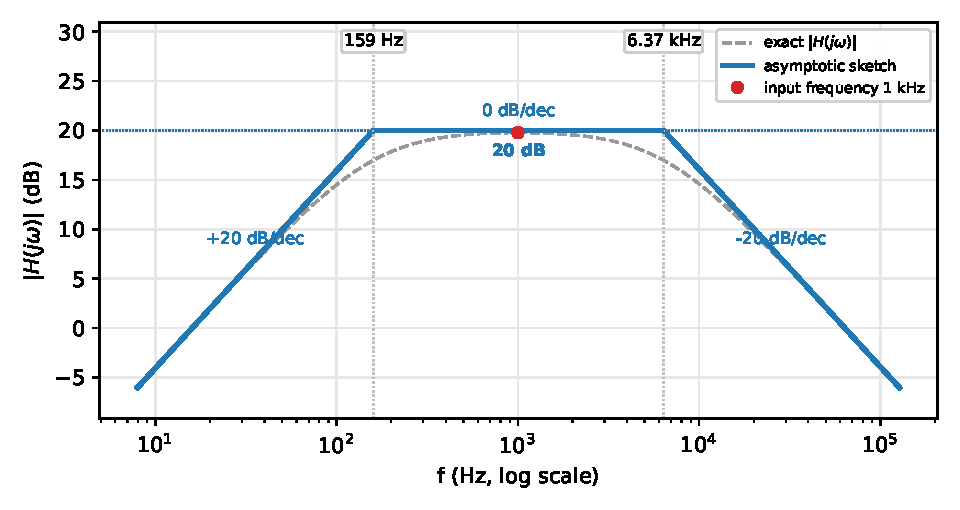
\includegraphics[width=0.78\linewidth,height=6.5cm,keepaspectratio]{p15_bode}\end{center}

{\small Blue: the straight-line sketch you are expected to draw. Dashed grey: the exact curve (about 3\,dB below the corner of an isolated pole). Red dot: the input frequency of Step 7.}
\solstep{7}{Steady-state output}The input is $V_i(t) = 0.05\sin\left(2\pi\cdot 1000\,t\right)$, so $\omega_{in} = 2\pi\cdot 1000 = 6280$\,rad/s. Put $s=j\omega_{in}$ in each factor (tool T5): magnitudes multiply, angles add.
{\small Rules: $\left|\frac{s}{s+p}\right| = \frac{\omega}{\sqrt{\omega^2+p^2}}$, $\angle = \frac{\pi}{2}-\tan^{-1}\frac{\omega}{p}$;\quad $\left|\frac{1}{1+s/p}\right| = \frac{1}{\sqrt{1+(\omega/p)^2}}$, $\angle = -\tan^{-1}\frac{\omega}{p}$;\quad $\left|1+\frac{s}{z}\right| = \sqrt{1+(\omega/z)^2}$, $\angle = \tan^{-1}\frac{\omega}{z}$;\quad a negative $K$ adds $-\pi$.}
\begin{center}\renewcommand{\arraystretch}{1.35}
\begin{tabular}{ccc}
\toprule
factor & magnitude & angle (rad) \\
\midrule
$-10$ & $10$ & $-3.14$ \\
$\rule[-1.1em]{0pt}{2.8em}\dfrac{s}{s+2\pi\cdot 159}$ & $0.9876$ & $0.158$ \\
$\rule[-1.7em]{0pt}{4em}\dfrac{1}{1+\dfrac{s}{2\pi\cdot 6.37\mathrm{k}}}$ & $0.9879$ & $-0.156$ \\
\textbf{total} & $\mathbf{9.756}$ (product) & $\mathbf{-3.14}$ (sum) \\
\bottomrule
\end{tabular}\end{center}

\begin{align*}
|H(j\omega_{in})| &= 9.76, \qquad \angle H(j\omega_{in}) = -3.14\ \mathrm{rad} \\
v_{o,ac}(t) &= 9.76\times 0.05\,\sin\left(2\pi\cdot 1000\,t - 3.14\right) = 0.488\,\sin\left(2\pi\cdot 1000\,t - 3.14\right)
\end{align*}

\[
\boxed{V_o(t) = 0.488\,\sin\left(2\pi\cdot 1000\,t - 3.14\right)\ \mathrm{V}}
\]

\begin{ansbox}
$H(s) = -10\,\dfrac{s}{s+2\pi\cdot 159}\,\dfrac{1}{1+\dfrac{s}{2\pi\cdot 6.37\mathrm{k}}}$\quad (corners: 159 Hz, 6.37 kHz)\\[4pt]
$V_o(t) = 0.488\,\sin\left(2\pi\cdot 1000\,t - 3.14\right)\ \mathrm{V}$
\end{ansbox}

\newpage
\subsection*{Solution 2B.16 \hfill Hard}
\begin{center}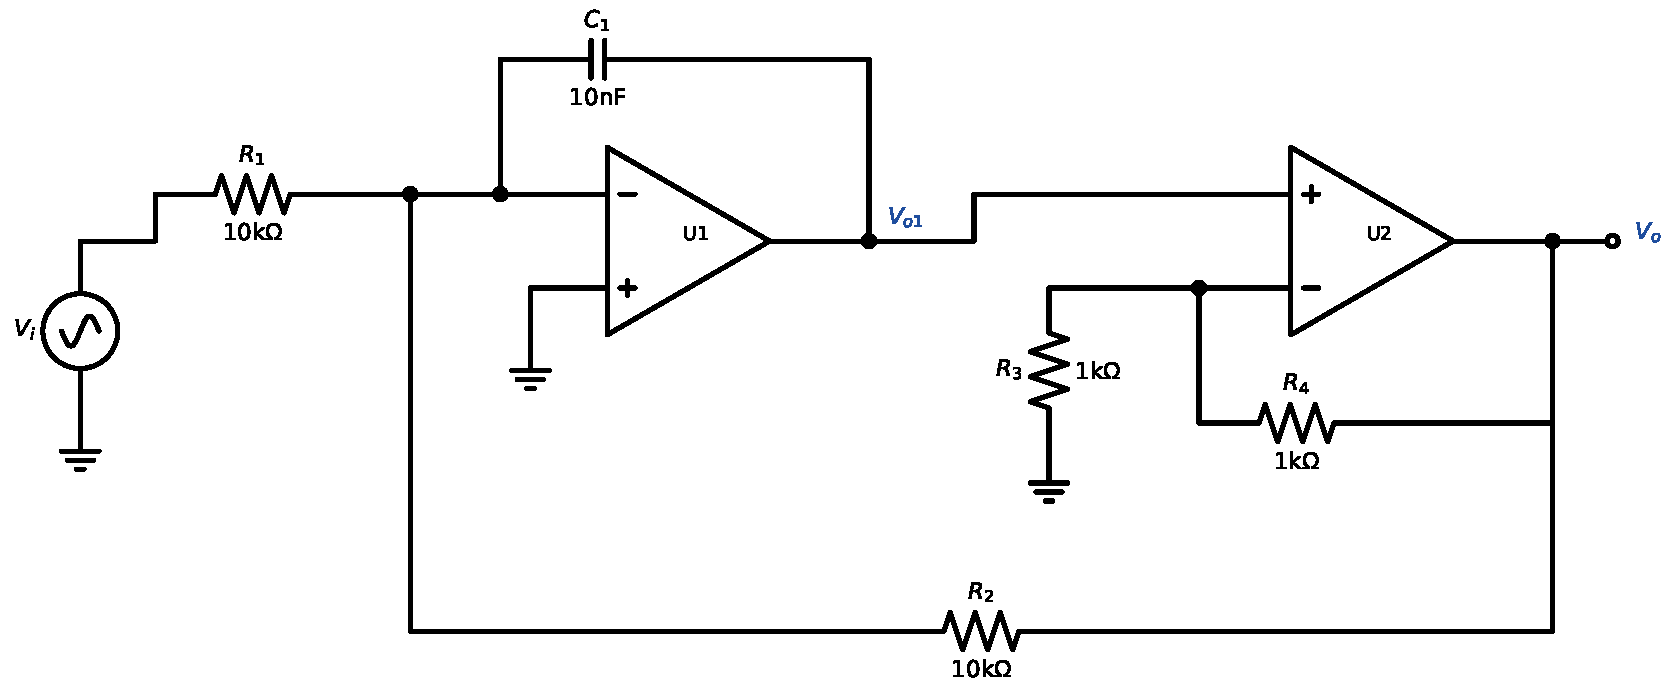
\includegraphics[width=\linewidth,height=5cm,keepaspectratio]{p16_circuit}\end{center}
\solstep{1}{Identify the sources}Independent sources: the AC input $V_i(t)$. No DC source: $V_{o,dc}=0$ and Step 2 is skipped.
\solstep{2}{DC circuit}No DC sources: $V_{o,dc}=0$.
\solstep{3}{Op-amp rules}Each op-amp has negative feedback (its output is connected back to its $-$ input), so with an ideal op-amp (tool T1): (a) no current flows into the $+$ or $-$ input; (b) $V_-=V_+$ (virtual short). The circuit is not a standard block, so it is solved by nodal analysis (tools T3, T4).
\solstep{4}{Transfer function by nodal analysis}\textbf{Block 1 (U1).} Two op-amps in a loop: $U_2$ amplifies $V_{o1}$ and feeds it back into the summing node of $U_1$, so the stages cannot simply be multiplied. This is not a standard block, so use nodal analysis. Virtual short (tool T1): U1: $V_- = V_+$, so $V_{-}$ is the same voltage as $0$ (virtual ground). U2: $V_- = V_+$, so $V_{n}$ is the same voltage as $V_{o1}$.
KCL (tool T3) at every node that is not an op-amp output or a source; no current flows into the op-amp inputs, so the op-amps do not appear in these sums:
\begin{align*}
&\text{(1) at }V_{-}\,(=0): && \frac{0 - V_{i}}{R_{1}} + sC_{1}\left(0 - V_{o1}\right) + \frac{0 - V_{o}}{R_{2}} = 0 \\
&\text{(2) at }V_{n}\,(=V_{o1}): && \frac{V_{o1}}{R_{3}} + \frac{V_{o1} - V_{o}}{R_{4}} = 0
\end{align*}

Solve them one at a time (tool T4): take the equation with the fewest unknowns, solve it for one node voltage and substitute that into the remaining equations. With the component values:
\begin{align*}
\text{from (1):}\quad V_{o1} &= \left(\dfrac{-10000}{s}\right)V_{o} + \left(\dfrac{-10000}{s}\right)V_i
\end{align*}

Substituting everything into (2) leaves only $V_{o}$ and $V_i$.\[
\frac{V_{o}}{V_i} = \dfrac{-20000}{s + 20000}
\]

So:\[
H(s) = \dfrac{-20000}{s + 20000}
\]

\solstep{5}{Standard (Bode-ready) form}Find the roots. Every root $s=-p$ of the denominator is a \emph{pole}, every root $s=-z$ of the numerator is a \emph{zero}; $|p|$ and $|z|$ are the corner frequencies (rad/s).
\begin{itemize}[leftmargin=*,itemsep=2pt]
\item Denominator: $s + 20000$; $s + 20000 = 0 \Rightarrow s = -20000$.
\end{itemize}

Factored form (leading coefficient in front):
\[
H(s) = -20000\,\dfrac{1}{(s+20000)}
\]

Bode-ready form: rewrite every $(s+p) = p\left(1+\frac{s}{p}\right)$ and $(s+z) = z\left(1+\frac{s}{z}\right)$, and collect all constants into $K$. Then every factor except $K$ is $\approx 1$ inside the pass-band:
\[
H(s) = -1\,\dfrac{1}{1+\dfrac{s}{2\pi\cdot 3.18\mathrm{k}}},\qquad K = -1
\]

\begin{center}\renewcommand{\arraystretch}{1.35}
\begin{tabular}{cccc}
\toprule
type & $\omega_c$ (rad/s) & $f_c=\omega_c/2\pi$ & slope change \\
\midrule
pole & $20000$ & 3.18 kHz & $-20$ dB/dec \\
\bottomrule
\end{tabular}\end{center}

\solstep{6}{Magnitude Bode plot}Below every corner, all factors are $\approx$ constant: $|H| \approx 1$ $= 0$\,dB (flat, 0 dB/dec). Then, moving right, each pole bends the line down by 20\,dB/dec and each zero bends it up by 20\,dB/dec (tool T6):
\begin{center}\renewcommand{\arraystretch}{1.35}
\begin{tabular}{lcl}
\toprule
frequency range & slope & asymptote level \\
\midrule
$f<$ 3.18 kHz & $0$ dB/dec (flat) & 0 dB at end \\
$f>$ 3.18 kHz & $-20$ dB/dec & 0 dB at start \\
\bottomrule
\end{tabular}\end{center}

The flat (pass-band) level is $20\log_{10}|K| = 20\log_{10}1 = 0$\,dB.
\begin{center}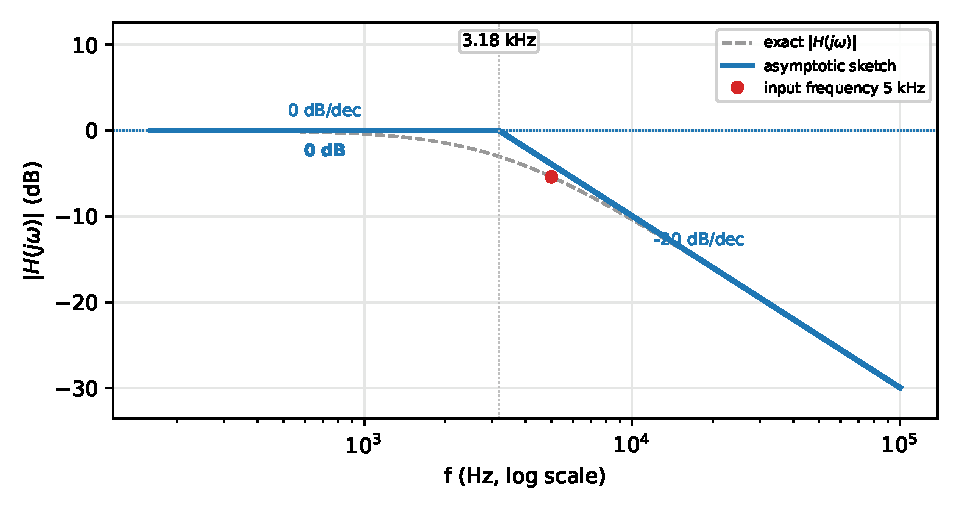
\includegraphics[width=0.78\linewidth,height=6.5cm,keepaspectratio]{p16_bode}\end{center}

{\small Blue: the straight-line sketch you are expected to draw. Dashed grey: the exact curve (about 3\,dB below the corner of an isolated pole). Red dot: the input frequency of Step 7.}
\solstep{7}{Steady-state output}The input is $V_i(t) = 0.2\cos\left(2\pi\cdot 5000\,t-\frac{\pi}{4}\right)$, so $\omega_{in} = 2\pi\cdot 5000 = 31400$\,rad/s. Put $s=j\omega_{in}$ in each factor (tool T5): magnitudes multiply, angles add.
{\small Rules: $\left|\frac{s}{s+p}\right| = \frac{\omega}{\sqrt{\omega^2+p^2}}$, $\angle = \frac{\pi}{2}-\tan^{-1}\frac{\omega}{p}$;\quad $\left|\frac{1}{1+s/p}\right| = \frac{1}{\sqrt{1+(\omega/p)^2}}$, $\angle = -\tan^{-1}\frac{\omega}{p}$;\quad $\left|1+\frac{s}{z}\right| = \sqrt{1+(\omega/z)^2}$, $\angle = \tan^{-1}\frac{\omega}{z}$;\quad a negative $K$ adds $-\pi$.}
\begin{center}\renewcommand{\arraystretch}{1.35}
\begin{tabular}{ccc}
\toprule
factor & magnitude & angle (rad) \\
\midrule
$-1$ & $1$ & $-3.14$ \\
$\rule[-1.7em]{0pt}{4em}\dfrac{1}{1+\dfrac{s}{2\pi\cdot 3.18\mathrm{k}}}$ & $0.537$ & $-1$ \\
\textbf{total} & $\mathbf{0.537}$ (product) & $\mathbf{-4.15}$ (sum) \\
\bottomrule
\end{tabular}\end{center}

\begin{align*}
|H(j\omega_{in})| &= 0.537, \qquad \angle H(j\omega_{in}) = -4.15\ \mathrm{rad} \\
v_{o,ac}(t) &= 0.537\times 0.2\,\cos\left(2\pi\cdot 5000\,t - 4.93\right) = 0.107\,\cos\left(2\pi\cdot 5000\,t - 4.93\right)
\end{align*}

(phase: $\theta + \angle H = -\frac{\pi}{4} + (-4.15) = -4.93$\,rad.)
\[
\boxed{V_o(t) = 0.107\,\cos\left(2\pi\cdot 5000\,t - 4.93\right)\ \mathrm{V}}
\]

\begin{ansbox}
$H(s) = -1\,\dfrac{1}{1+\dfrac{s}{2\pi\cdot 3.18\mathrm{k}}}$\quad (corners: 3.18 kHz)\\[4pt]
$V_o(t) = 0.107\,\cos\left(2\pi\cdot 5000\,t - 4.93\right)\ \mathrm{V}$
\end{ansbox}

\newpage
\subsection*{Solution 2B.17 \hfill Hard}
\begin{center}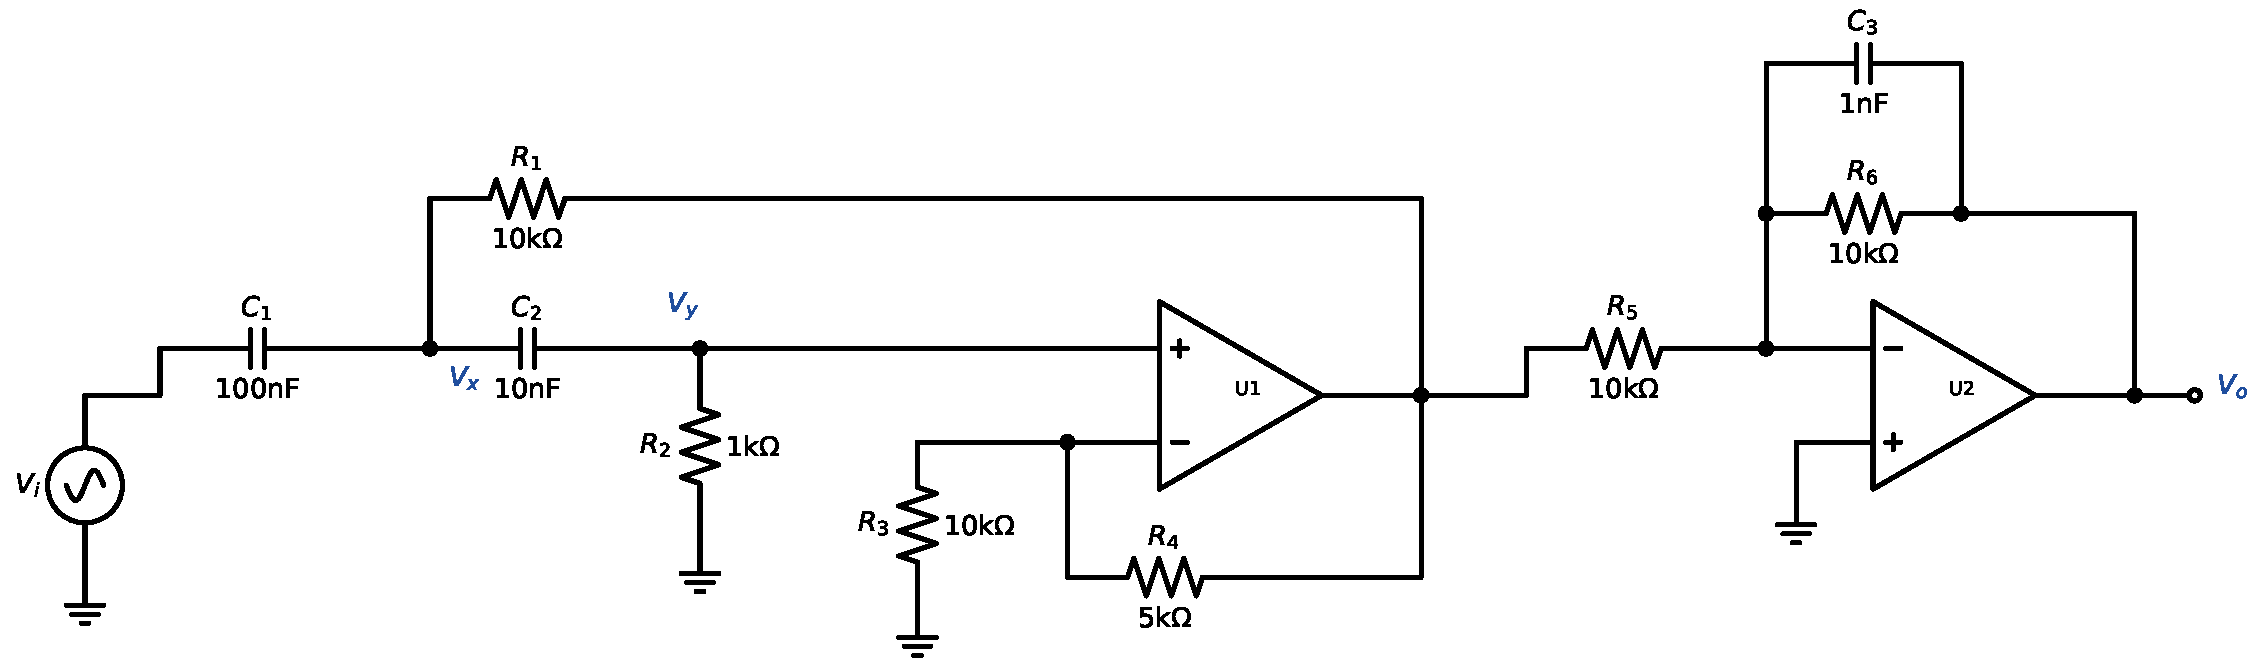
\includegraphics[width=\linewidth,height=5cm,keepaspectratio]{p17_circuit}\end{center}
\solstep{1}{Identify the sources}Independent sources: the AC input $V_i(t)$. No DC source: $V_{o,dc}=0$ and Step 2 is skipped.
\solstep{2}{DC circuit}No DC sources: $V_{o,dc}=0$.
\solstep{3}{Op-amp rules}Each op-amp has negative feedback (its output is connected back to its $-$ input), so with an ideal op-amp (tool T1): (a) no current flows into the $+$ or $-$ input; (b) $V_-=V_+$ (virtual short). Block 1 is not a standard block (nodal analysis, tools T3 and T4); the other blocks are standard (block formulas, tool T2). The blocks still multiply because every op-amp output is an ideal source.
\solstep{4}{Transfer function, block by block}Each op-amp output is an ideal voltage source, so a block's output does not change when the next block is connected: the blocks can be solved one at a time and multiplied.\[
H(s) = \frac{V_o}{V_i} = \frac{V_{o1}}{V_{i}}\cdot\frac{V_{o}}{V_{o1}}
\]

\textbf{Block 1 (U1).} Sallen-Key stage: the network feeds back from the output to node $V_x$. This is not a standard block, so use nodal analysis. Virtual short (tool T1): U1: $V_- = V_+$, so $V_{-}$ is the same voltage as $V_{y}$.
KCL (tool T3) at every node that is not an op-amp output or a source; no current flows into the op-amp inputs, so the op-amps do not appear in these sums:
\begin{align*}
&\text{(1) at }V_{-}\,(=V_{y}): && \frac{V_{y}}{R_{3}} + \frac{V_{y} - V_{o1}}{R_{4}} = 0 \\
&\text{(2) at }V_{x}: && sC_{1}\left(V_{x} - V_{i}\right) + sC_{2}\left(V_{x} - V_{y}\right) + \frac{V_{x} - V_{o1}}{R_{1}} = 0 \\
&\text{(3) at }V_{y}: && sC_{2}\left(V_{y} - V_{x}\right) + \frac{V_{y}}{R_{2}} = 0
\end{align*}

Solve them one at a time (tool T4): take the equation with the fewest unknowns, solve it for one node voltage and substitute that into the remaining equations. With the component values:
\begin{align*}
\text{from (1):}\quad V_{y} &= 0.667\,V_{o1} \\
\text{from (2):}\quad V_{x} &= \left(\dfrac{0.0606\,s + 909}{s + 909}\right)V_{o1} + \left(\dfrac{0.909\,s}{s + 909}\right)V_i
\end{align*}

Substituting everything into (3) leaves only $V_{o1}$ and $V_i$.\[
\frac{V_{o1}}{V_i} = \dfrac{1.5\,s^{2}}{s^{2} + 1.09\times 10^{5}\,s + 10^{8}}
\]

\textbf{Block 2 (U2).} Inverting block: the $+$ input is grounded, so $V_- = V_+ = 0$ (virtual ground). The current $\frac{V_{o1} - 0}{R_{5}}$ through $R_{5}$ cannot enter the op-amp, so all of it flows through $Z_{f2}$: $V_{o} = 0 - Z_{f2}\cdot\frac{V_{o1}}{R_{5}}$.\begin{align*}
Z_{f2} &= R_{6} \parallel \frac{1}{sC_{3}} = \dfrac{10^{9}}{s + 10^{5}}
\end{align*}
\[
\frac{V_{o}}{V_{o1}} = -\frac{Z_{f2}}{R_{5}} = \dfrac{-10^{5}}{s + 10^{5}}
\]

Multiply the blocks and simplify:\[
H(s) = \dfrac{-1.5\times 10^{5}\,s^{2}}{s^{3} + 2.1\times 10^{5}\,s^{2} + 1.1\times 10^{10}\,s + 10^{13}}
\]

\solstep{5}{Standard (Bode-ready) form}Find the roots. Every root $s=-p$ of the denominator is a \emph{pole}, every root $s=-z$ of the numerator is a \emph{zero}; $|p|$ and $|z|$ are the corner frequencies (rad/s).
\begin{itemize}[leftmargin=*,itemsep=2pt]
\item Numerator: it has the factor $s^2$ $\Rightarrow$ 2 zeros at $s=0$.
\item Denominator: $s^{3} + 2.1\times 10^{5}\,s^{2} + 1.1\times 10^{10}\,s + 10^{13}$; this is degree 3: use a calculator's polynomial solver (or \texttt{numpy.roots}) $\Rightarrow s = -921,\ -100000,\ -1.09\times 10^{5}$.
\end{itemize}

Factored form (leading coefficient in front):
\[
H(s) = -1.5\times 10^{5}\,\dfrac{s^{2}}{(s+921)(s+10^{5})(s+1.09\times 10^{5})}
\]

Bode-ready form: rewrite every $(s+p) = p\left(1+\frac{s}{p}\right)$ and $(s+z) = z\left(1+\frac{s}{z}\right)$, and collect all constants into $K$. Each $s$ in the numerator is paired with one of the \emph{lowest} poles as $\frac{s}{s+p}$ (that factor is $\approx 1$ above $p$). Then every factor except $K$ is $\approx 1$ inside the pass-band:
\[
H(s) = -1.38\,\dfrac{s}{s+2\pi\cdot 147}\,\dfrac{s}{s+2\pi\cdot 15.9\mathrm{k}}\,\dfrac{1}{1+\dfrac{s}{2\pi\cdot 17.3\mathrm{k}}},\qquad K = -1.38
\]

\begin{center}\renewcommand{\arraystretch}{1.35}
\begin{tabular}{cccc}
\toprule
type & $\omega_c$ (rad/s) & $f_c=\omega_c/2\pi$ & slope change \\
\midrule
pole & $921$ & 147 Hz & $-20$ dB/dec \\
pole & $10^{5}$ & 15.9 kHz & $-20$ dB/dec \\
pole & $1.09\times 10^{5}$ & 17.3 kHz & $-20$ dB/dec \\
\bottomrule
\end{tabular}\end{center}

\solstep{6}{Magnitude Bode plot}Below every corner $|H(s)|\approx 1.5\times 10^{-8}\,s^2$, so the plot starts with a slope of $+40$\,dB/dec. Then, moving right, each pole bends the line down by 20\,dB/dec and each zero bends it up by 20\,dB/dec (tool T6):
\begin{center}\renewcommand{\arraystretch}{1.35}
\begin{tabular}{lcl}
\toprule
frequency range & slope & asymptote level \\
\midrule
$f<$ 147 Hz & $+40$ dB/dec & -37.9 dB at end \\
147 Hz -- 15.9 kHz & $+20$ dB/dec & -37.9 dB at start, 2.81 dB at end \\
15.9 kHz -- 17.3 kHz & $0$ dB/dec (flat) & 2.81 dB at start, 2.81 dB at end \\
$f>$ 17.3 kHz & $-20$ dB/dec & 2.81 dB at start \\
\bottomrule
\end{tabular}\end{center}

The flat (pass-band) level is $20\log_{10}|K| = 20\log_{10}1.38 = 2.81$\,dB.
\begin{center}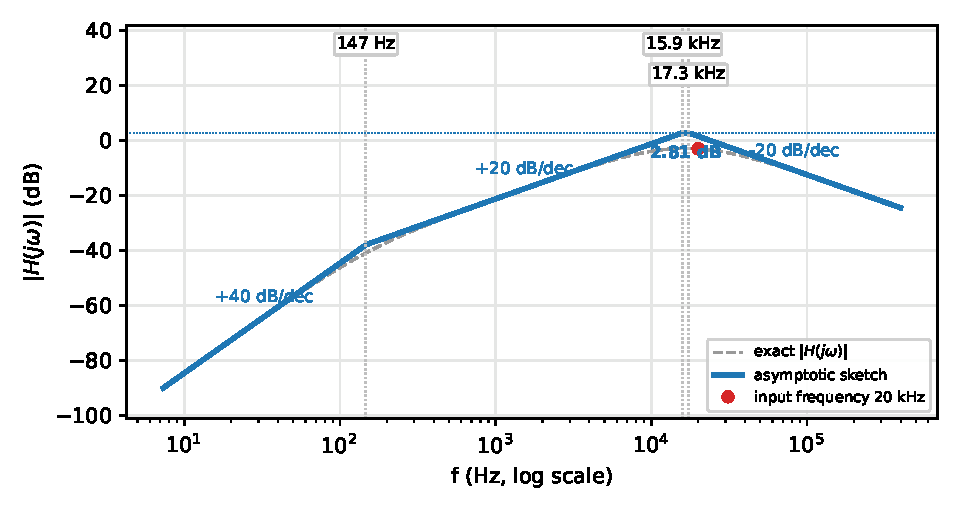
\includegraphics[width=0.78\linewidth,height=6.5cm,keepaspectratio]{p17_bode}\end{center}

{\small Blue: the straight-line sketch you are expected to draw. Dashed grey: the exact curve (about 3\,dB below the corner of an isolated pole). Red dot: the input frequency of Step 7.}
\solstep{7}{Steady-state output}The input is $V_i(t) = 0.1\sin\left(2\pi\cdot 20000\,t\right)$, so $\omega_{in} = 2\pi\cdot 20000 = 1.26\times 10^{5}$\,rad/s. Put $s=j\omega_{in}$ in each factor (tool T5): magnitudes multiply, angles add.
{\small Rules: $\left|\frac{s}{s+p}\right| = \frac{\omega}{\sqrt{\omega^2+p^2}}$, $\angle = \frac{\pi}{2}-\tan^{-1}\frac{\omega}{p}$;\quad $\left|\frac{1}{1+s/p}\right| = \frac{1}{\sqrt{1+(\omega/p)^2}}$, $\angle = -\tan^{-1}\frac{\omega}{p}$;\quad $\left|1+\frac{s}{z}\right| = \sqrt{1+(\omega/z)^2}$, $\angle = \tan^{-1}\frac{\omega}{z}$;\quad a negative $K$ adds $-\pi$.}
\begin{center}\renewcommand{\arraystretch}{1.35}
\begin{tabular}{ccc}
\toprule
factor & magnitude & angle (rad) \\
\midrule
$-1.38$ & $1.381$ & $-3.14$ \\
$\rule[-1.1em]{0pt}{2.8em}\dfrac{s}{s+2\pi\cdot 147}$ & $1$ & $0.00733$ \\
$\rule[-1.1em]{0pt}{2.8em}\dfrac{s}{s+2\pi\cdot 15.9\mathrm{k}}$ & $0.7825$ & $0.672$ \\
$\rule[-1.7em]{0pt}{4em}\dfrac{1}{1+\dfrac{s}{2\pi\cdot 17.3\mathrm{k}}}$ & $0.6538$ & $-0.858$ \\
\textbf{total} & $\mathbf{0.7067}$ (product) & $\mathbf{-3.32}$ (sum) \\
\bottomrule
\end{tabular}\end{center}

\begin{align*}
|H(j\omega_{in})| &= 0.707, \qquad \angle H(j\omega_{in}) = -3.32\ \mathrm{rad} \\
v_{o,ac}(t) &= 0.707\times 0.1\,\sin\left(2\pi\cdot 20000\,t - 3.32\right) = 0.0707\,\sin\left(2\pi\cdot 20000\,t - 3.32\right)
\end{align*}

\[
\boxed{V_o(t) = 0.0707\,\sin\left(2\pi\cdot 20000\,t - 3.32\right)\ \mathrm{V}}
\]

\begin{ansbox}
$H(s) = -1.38\,\dfrac{s}{s+2\pi\cdot 147}\,\dfrac{s}{s+2\pi\cdot 15.9\mathrm{k}}\,\dfrac{1}{1+\dfrac{s}{2\pi\cdot 17.3\mathrm{k}}}$\quad (corners: 147 Hz, 15.9 kHz, 17.3 kHz)\\[4pt]
$V_o(t) = 0.0707\,\sin\left(2\pi\cdot 20000\,t - 3.32\right)\ \mathrm{V}$
\end{ansbox}

\newpage
\subsection*{Solution 2B.18 \hfill Hard}
\begin{center}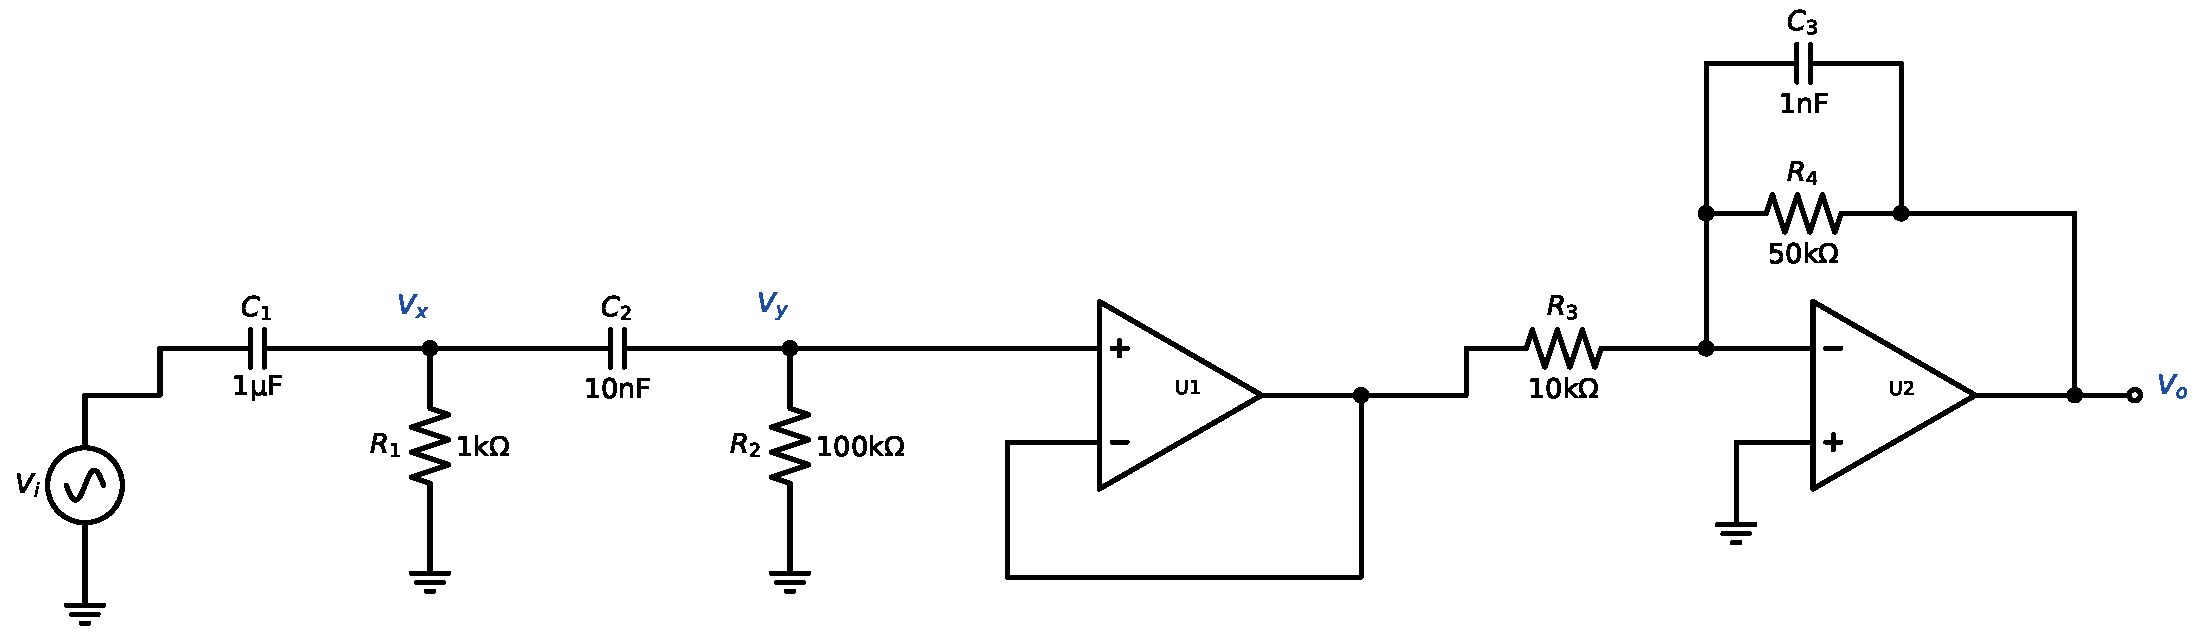
\includegraphics[width=\linewidth,height=5cm,keepaspectratio]{p18_circuit}\end{center}
\solstep{1}{Identify the sources}Independent sources: the AC input $V_i(t)$. No DC source: $V_{o,dc}=0$ and Step 2 is skipped.
\solstep{2}{DC circuit}No DC sources: $V_{o,dc}=0$.
\solstep{3}{Op-amp rules}Each op-amp has negative feedback (its output is connected back to its $-$ input), so with an ideal op-amp (tool T1): (a) no current flows into the $+$ or $-$ input; (b) $V_-=V_+$ (virtual short). Block 1 is not a standard block (nodal analysis, tools T3 and T4); the other blocks are standard (block formulas, tool T2). The blocks still multiply because every op-amp output is an ideal source.
\solstep{4}{Transfer function, block by block}Each op-amp output is an ideal voltage source, so a block's output does not change when the next block is connected: the blocks can be solved one at a time and multiplied.\[
H(s) = \frac{V_o}{V_i} = \frac{V_{o1}}{V_{i}}\cdot\frac{V_{o}}{V_{o1}}
\]

\textbf{Block 1 (U1).} A two-section passive ladder drives the $+$ input. This is not a standard block, so use nodal analysis. Virtual short (tool T1): U1: $V_- = V_+$, so $V_{o1}$ is the same voltage as $V_{y}$.
KCL (tool T3) at every node that is not an op-amp output or a source; no current flows into the op-amp inputs, so the op-amps do not appear in these sums:
\begin{align*}
&\text{(1) at }V_{x}: && sC_{1}\left(V_{x} - V_{i}\right) + \frac{V_{x}}{R_{1}} + sC_{2}\left(V_{x} - V_{y}\right) = 0 \\
&\text{(2) at }V_{y}: && sC_{2}\left(V_{y} - V_{x}\right) + \frac{V_{y}}{R_{2}} = 0
\end{align*}

Solve them one at a time (tool T4): take the equation with the fewest unknowns, solve it for one node voltage and substitute that into the remaining equations. With the component values:
\begin{align*}
\text{from (1):}\quad V_{x} &= \left(\dfrac{0.0099\,s}{s + 990}\right)V_{y} + \left(\dfrac{0.99\,s}{s + 990}\right)V_i
\end{align*}

Substituting everything into (2) leaves only $V_{y}$ and $V_i$. Since $V_{o1} = V_{y}$ (virtual short),\[
\frac{V_{o1}}{V_i} = \frac{V_{y}}{V_i} = \dfrac{s^{2}}{s^{2} + 2010\,s + 10^{6}}
\]

\textbf{Block 2 (U2).} Inverting block: the $+$ input is grounded, so $V_- = V_+ = 0$ (virtual ground). The current $\frac{V_{o1} - 0}{R_{3}}$ through $R_{3}$ cannot enter the op-amp, so all of it flows through $Z_{f2}$: $V_{o} = 0 - Z_{f2}\cdot\frac{V_{o1}}{R_{3}}$.\begin{align*}
Z_{f2} &= R_{4} \parallel \frac{1}{sC_{3}} = \dfrac{10^{9}}{s + 20000}
\end{align*}
\[
\frac{V_{o}}{V_{o1}} = -\frac{Z_{f2}}{R_{3}} = \dfrac{-10^{5}}{s + 20000}
\]

Multiply the blocks and simplify:\[
H(s) = \dfrac{-10^{5}\,s^{2}}{s^{3} + 22000\,s^{2} + 4.12\times 10^{7}\,s + 2\times 10^{10}}
\]

\solstep{5}{Standard (Bode-ready) form}Find the roots. Every root $s=-p$ of the denominator is a \emph{pole}, every root $s=-z$ of the numerator is a \emph{zero}; $|p|$ and $|z|$ are the corner frequencies (rad/s).
\begin{itemize}[leftmargin=*,itemsep=2pt]
\item Numerator: it has the factor $s^2$ $\Rightarrow$ 2 zeros at $s=0$.
\item Denominator: $s^{3} + 22000\,s^{2} + 4.12\times 10^{7}\,s + 2\times 10^{10}$; this is degree 3: use a calculator's polynomial solver (or \texttt{numpy.roots}) $\Rightarrow s = -905,\ -1110,\ -20000$.
\end{itemize}

Factored form (leading coefficient in front):
\[
H(s) = -10^{5}\,\dfrac{s^{2}}{(s+905)(s+1110)(s+20000)}
\]

Bode-ready form: rewrite every $(s+p) = p\left(1+\frac{s}{p}\right)$ and $(s+z) = z\left(1+\frac{s}{z}\right)$, and collect all constants into $K$. Each $s$ in the numerator is paired with one of the \emph{lowest} poles as $\frac{s}{s+p}$ (that factor is $\approx 1$ above $p$). Then every factor except $K$ is $\approx 1$ inside the pass-band:
\[
H(s) = -5\,\dfrac{s}{s+2\pi\cdot 144}\,\dfrac{s}{s+2\pi\cdot 176}\,\dfrac{1}{1+\dfrac{s}{2\pi\cdot 3.18\mathrm{k}}},\qquad K = -5
\]

\begin{center}\renewcommand{\arraystretch}{1.35}
\begin{tabular}{cccc}
\toprule
type & $\omega_c$ (rad/s) & $f_c=\omega_c/2\pi$ & slope change \\
\midrule
pole & $905$ & 144 Hz & $-20$ dB/dec \\
pole & $1110$ & 176 Hz & $-20$ dB/dec \\
pole & $20000$ & 3.18 kHz & $-20$ dB/dec \\
\bottomrule
\end{tabular}\end{center}

\solstep{6}{Magnitude Bode plot}Below every corner $|H(s)|\approx 5\times 10^{-6}\,s^2$, so the plot starts with a slope of $+40$\,dB/dec. Then, moving right, each pole bends the line down by 20\,dB/dec and each zero bends it up by 20\,dB/dec (tool T6):
\begin{center}\renewcommand{\arraystretch}{1.35}
\begin{tabular}{lcl}
\toprule
frequency range & slope & asymptote level \\
\midrule
$f<$ 144 Hz & $+40$ dB/dec & 12.2 dB at end \\
144 Hz -- 176 Hz & $+20$ dB/dec & 12.2 dB at start, 14 dB at end \\
176 Hz -- 3.18 kHz & $0$ dB/dec (flat) & 14 dB at start, 14 dB at end \\
$f>$ 3.18 kHz & $-20$ dB/dec & 14 dB at start \\
\bottomrule
\end{tabular}\end{center}

The flat (pass-band) level is $20\log_{10}|K| = 20\log_{10}5 = 14$\,dB.
\begin{center}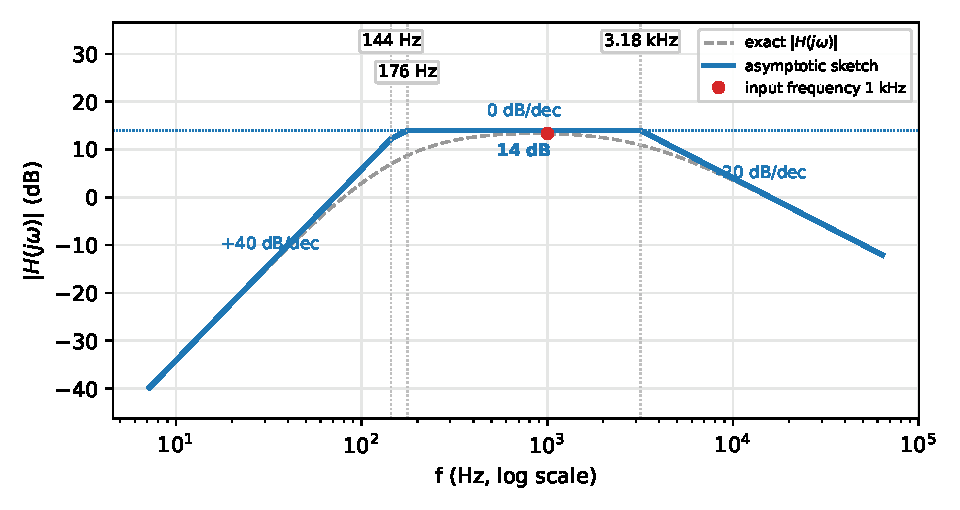
\includegraphics[width=0.78\linewidth,height=6.5cm,keepaspectratio]{p18_bode}\end{center}

{\small Blue: the straight-line sketch you are expected to draw. Dashed grey: the exact curve (about 3\,dB below the corner of an isolated pole). Red dot: the input frequency of Step 7.}
\solstep{7}{Steady-state output}The input is $V_i(t) = 0.05\sin\left(2\pi\cdot 1000\,t+\frac{\pi}{3}\right)$, so $\omega_{in} = 2\pi\cdot 1000 = 6280$\,rad/s. Put $s=j\omega_{in}$ in each factor (tool T5): magnitudes multiply, angles add.
{\small Rules: $\left|\frac{s}{s+p}\right| = \frac{\omega}{\sqrt{\omega^2+p^2}}$, $\angle = \frac{\pi}{2}-\tan^{-1}\frac{\omega}{p}$;\quad $\left|\frac{1}{1+s/p}\right| = \frac{1}{\sqrt{1+(\omega/p)^2}}$, $\angle = -\tan^{-1}\frac{\omega}{p}$;\quad $\left|1+\frac{s}{z}\right| = \sqrt{1+(\omega/z)^2}$, $\angle = \tan^{-1}\frac{\omega}{z}$;\quad a negative $K$ adds $-\pi$.}
\begin{center}\renewcommand{\arraystretch}{1.35}
\begin{tabular}{ccc}
\toprule
factor & magnitude & angle (rad) \\
\midrule
$-5$ & $5$ & $-3.14$ \\
$\rule[-1.1em]{0pt}{2.8em}\dfrac{s}{s+2\pi\cdot 144}$ & $0.9898$ & $0.143$ \\
$\rule[-1.1em]{0pt}{2.8em}\dfrac{s}{s+2\pi\cdot 176}$ & $0.9849$ & $0.174$ \\
$\rule[-1.7em]{0pt}{4em}\dfrac{1}{1+\dfrac{s}{2\pi\cdot 3.18\mathrm{k}}}$ & $0.954$ & $-0.304$ \\
\textbf{total} & $\mathbf{4.65}$ (product) & $\mathbf{-3.13}$ (sum) \\
\bottomrule
\end{tabular}\end{center}

\begin{align*}
|H(j\omega_{in})| &= 4.65, \qquad \angle H(j\omega_{in}) = -3.13\ \mathrm{rad} \\
v_{o,ac}(t) &= 4.65\times 0.05\,\sin\left(2\pi\cdot 1000\,t - 2.08\right) = 0.233\,\sin\left(2\pi\cdot 1000\,t - 2.08\right)
\end{align*}

(phase: $\theta + \angle H = \frac{\pi}{3} + (-3.13) = -2.08$\,rad.)
\[
\boxed{V_o(t) = 0.233\,\sin\left(2\pi\cdot 1000\,t - 2.08\right)\ \mathrm{V}}
\]

\begin{ansbox}
$H(s) = -5\,\dfrac{s}{s+2\pi\cdot 144}\,\dfrac{s}{s+2\pi\cdot 176}\,\dfrac{1}{1+\dfrac{s}{2\pi\cdot 3.18\mathrm{k}}}$\quad (corners: 144 Hz, 176 Hz, 3.18 kHz)\\[4pt]
$V_o(t) = 0.233\,\sin\left(2\pi\cdot 1000\,t - 2.08\right)\ \mathrm{V}$
\end{ansbox}

\end{document}
